\documentclass{article}
\usepackage[ngerman]{babel}
\usepackage[utf8]{inputenc}
\usepackage{graphicx} 
\usepackage{epstopdf}
\usepackage{svg}
\usepackage{float}
\usepackage{booktabs}
\usepackage{longtable, lscape}
\usepackage{tikz}
\usepackage{multicol}
\usepackage{array} 
\usepackage{tabularx}
\usepackage{varwidth}
\graphicspath{{img/}}
\usepackage{geometry}
\usepackage{amsmath,mathtools}
\usepackage{acronym}
\usepackage{pdflscape}
\usepackage[hidelinks]{hyperref}
\hypersetup{
    colorlinks=false, %set true if you want colored links
    linktoc=all
}
\geometry{a4paper, top=25mm, left=30mm, right=25mm, bottom=20mm}
\usepackage{titlesec}
\usepackage[footsepline,headsepline]{scrpage2}
\setfootsepline{1pt}
\setheadsepline{1pt}
\pagestyle{scrheadings}
\clearscrheadfoot
\cfoot{\pagemark}
\chead{\headmark}
\automark[subsection]{section}
\titleclass{\subsubsubsection}{straight}[\subsection]

\usepackage[T1]{fontenc}


%Listing
\usepackage{courier}
\usepackage{listings}
\usepackage{color}
 \lstset{
   frame=tb,
   basicstyle=\footnotesize\bfseries\ttfamily,
   emph={square}, 
   emphstyle=\color{blue}\texttt,
   emph={[2]root,base},
   emphstyle={[2]\color{yac}\texttt},
   showstringspaces=false,
   flexiblecolumns=false,
   tabsize=2,
   numbers=left,
   numberstyle=\tiny\bfseries,
   numberblanklines=false,
   stepnumber=1,
   numbersep=10pt,
   xleftmargin=15pt
 }

\newcounter{subsubsubsection}[subsubsection]
\renewcommand\thesubsubsubsection{\thesubsubsection.\arabic{subsubsubsection}}
\renewcommand\theparagraph{\thesubsubsubsection.\arabic{paragraph}} % optional; useful if paragraphs are to be numbered

\titleformat{\subsubsubsection}
  {\normalfont\normalsize\bfseries}{\thesubsubsubsection}{1em}{}
\titlespacing*{\subsubsubsection}
{0pt}{3.25ex plus 1ex minus .2ex}{1.5ex plus .2ex}

\makeatletter
\renewcommand\paragraph{\@startsection{paragraph}{5}{\z@}%
  {3.25ex \@plus1ex \@minus.2ex}%
  {-1em}%
  {\normalfont\normalsize\bfseries}}
\renewcommand\subparagraph{\@startsection{subparagraph}{6}{\parindent}%
  {3.25ex \@plus1ex \@minus .2ex}%
  {-1em}%
  {\normalfont\normalsize\bfseries}}
\def\toclevel@subsubsubsection{4}
\def\toclevel@paragraph{5}
\def\toclevel@paragraph{6}
\def\l@subsubsubsection{\@dottedtocline{4}{7em}{4em}}
\def\l@paragraph{\@dottedtocline{5}{10em}{5em}}
\def\l@subparagraph{\@dottedtocline{6}{14em}{6em}}
\makeatother

\setcounter{secnumdepth}{4}
\setcounter{tocdepth}{4}

\newcommand{\inW}{\prescript{w}{}}
\newcommand{\inI}{\prescript{I}{}}
\newcommand{\bS}[1]{\boldsymbol{#1}}
\newcommand{\BinW}[1]{\inW{}\boldsymbol{#1}}
\newcommand{\BinI}[1]{\inI{}\boldsymbol{#1}}

\begin{document}

\begin{titlepage}
\title{\textbf{Cu}be-\textbf{Ba}lancing: Der selbst balancierende Würfel}
\author{Florian Roth, Michael Meindl, Alexander Sarici, Alexander Schleicher}
\date{\today}
\end{titlepage}

\clearpage
\setcounter{page}{1}
\pagenumbering{Roman}
\section*{Vorwort}
In der folgenden Dokumentation wird das \ac{CuBa}-Projekt vorgestellt, welches im Rahmen eines Entwicklungsprojektes an der Hochschule Karlsruhe durchgeführt wurde. Die Idee für dieses Projekt stammt von dem s.g. Cubli der ETH Zürich. Hierbei handelt es sich um einen Würfel, welcher in der Lage ist selbständig auf seine Ecken und Kanten zu springen und dort zu balancieren. Die Hauptaufgaben dieser Arbeiten bestehen darin einen solchen solchen Würfel zu konstruieren, passende Sensorik bzw. Aktorik auszuwählen und in Betrieb zunehmen und auf der Basis einer Systemanalyse einen Regelkreis zu entwerfen. 

\tableofcontents
\newpage

\section*{Abkürzungsverzeichnis}
\begin{acronym}
	\acro{CuBa}{Cube-Balancing}
	\acro{BBB}{BeagleBone Black}
	\acro{SHM}{Shared Memory}
\end{acronym}

\newpage
\setcounter{page}{1}
\pagenumbering{arabic}
\section{Einführung}

Messungen:
\begin{itemize}
\item Beschleunigung Sensor1 und Sensor2 bei 45 Grad
\item Beschleunigung Sensor1 und Sensor2 bei 30 Grad
\item Beschleunigung Sensor1 und Sensor2 bei 15 Grad
\item Beschleunigung Sensor1 und Sensor2 bei 0  Grad
\item Beschleunigung Sensor1 und Sensor2 bei -15 Grad
\item Beschleunigung Sensor1 und Sensor2 bei -30 Grad
\item Beschleunigung Sensor1 und Sensor2 bei -45 Grad
\item Winkelgeschwindigkeit Sensor1 und Sensor2 bei 0 rad/sec
\end{itemize}
\section{1D-Prototyp}
In diesem Teil wird der erste Prototyp vorgestellt. Hierbei handelt es sich um eine einzelne Würfelseite, welche mit Hilfe einer Achse gelagert ist. Dadurch wird die Bewegung des Systems auf zwei rotatorische Freiheitsgrade beschränkt, nämlich die Rotation um die Achse und die Bewegung der Schwungmasse relativ zu der Würfelseite. Mit Hilfe dieses Entwurfes kann die Dynamik und Anforderungen an die Komponenten an einem vereinfachten Modell untersucht werden. Aus diesen Ergebnisse können dann Rückschlüsse auf den Entwurf des endgültigen Würfels gezogen werden.
\newline


\begin{figure}[h!]
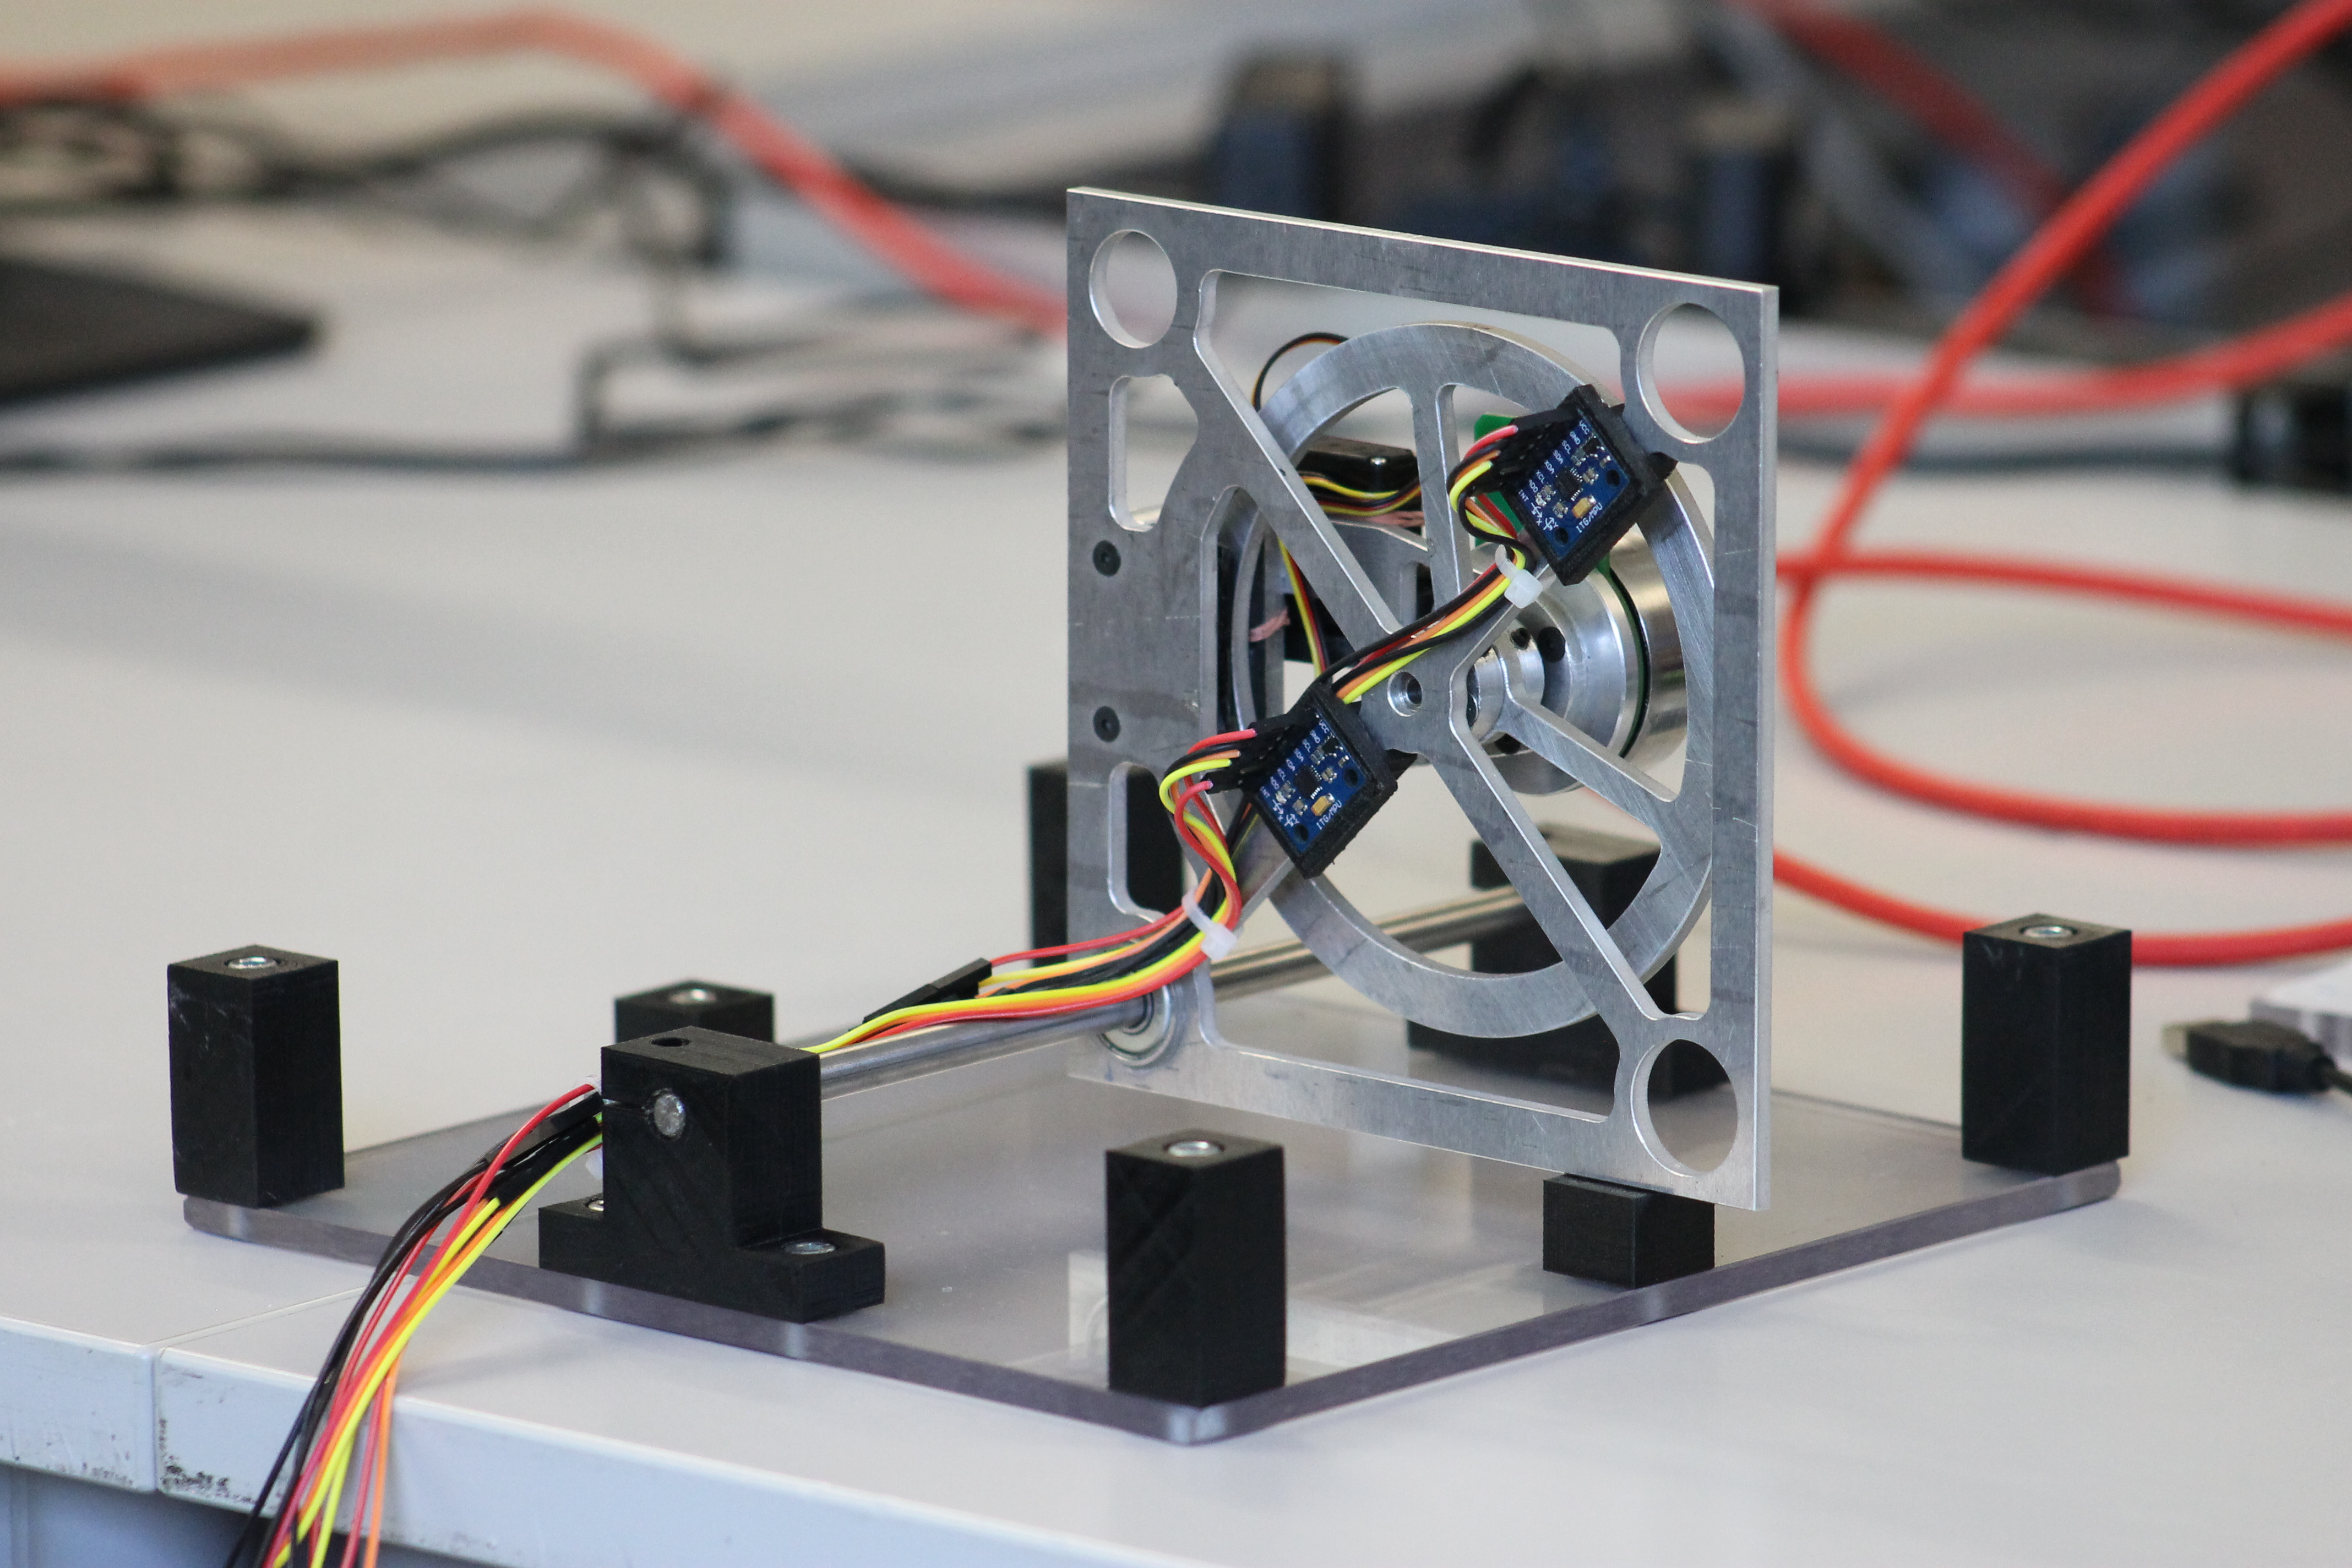
\includegraphics[width=\linewidth]{img/1D_Model_pic.JPG}
\caption{1D-Modell, Quelle: eigene Darstellung}
\end{figure}
\subsection{Aktorik und Sensorik}
Der folgenden Abschnitt beschreibt die verwendeten elektrischen Bauteile, um einerseits die benötigten physikalischen Größen zu messen, und andererseits die verwendete Aktorik, um das Aufspringen und Balancieren der Würfelseite zu ermöglichen.
\newline 

Die Aufgabe der Sensorik besteht darin die Zustandsgrößen des Systemes zu bestimmen. Hierfür werden zwei \textit{GYR-521}-Platinen verwendet, die mit einem \textit{MPU6050}-IC der Firma \textit{InvenSense} bestückt sind. Diese bieten jeweils einen dreiachsigen Beschleunigungssensor und Gyroskop. Mit Hilfe dieser Messwerte können die Zustandsgrößen $\varphi$ und $\dot{\varphi}$ berechnet werden. Die Sensoren bieten die zusätzliche Möglichkeit einen variablen Tiefpassfilter zu verwenden um eine erste Glättung der Messwerte durchzuführen. Dieses Tiefpassfilter wird auf eine Grenzfrequenz von $44Hz$ eingestellt. Dieser Wert hat sich empirisch als optimaler Kompromiss zwischen Filterung der Rauschsignale und Verzögerung des eigentlichen Signals ergeben. Die Konfiguration und Auswertung der Sensoren erfolgt über eine $I^2C$-Schnittstelle. Die Justierung und Auswertung der Sensoren wird näher in Abschnitt \ref{sensorik_sec} beschrieben.
\newline

Abschnitt \ref{Dynamik_sec} zeigt den Einfluss eines Motormomentes auf die Position und Gewschwindigkeit der Würfelseite. Um diese Moment zu erzeugen wird ein bürstenloser DC-Motor der Firma \textit{MaxonMotor} verwendet (EC 45 flat, 50 Watt). Die Kriterien zur Auswahl des Motors sind einerseits die maximale Drehzahl und Drehmoment, andererseits die mechanische Zeitkonstante. Für das Aufspringen des Würfels ist die maximale Drehzahl des Motors von Bedeutung, die 10000 Umdrehung pro Minute des gewählten Motor reichen hierbei aus um eine ausreichend hohe kinetische Energie der Schwungmasse zu ermöglichen. Die Robustheit der Regelung wird durch das maximale Drehmoment limitiert, welches in diesem Fall bei 83.4 mNm liegt. Von besondere Bedeutung für die Regelung ist die mechanische Zeitkonstante des Motors, da diese eine Verzögerung der Stellgröße bewirkt und somit den geschlossenen Regelkreis negativ beeinflussen kann. Die mechanische Zeitkonstante des gewählten Motors ist mit $13.3ms$ im Vergleich zu anderen Kandidaten sehr niedrig. Die Ansteuerung des Motors erfolgt über den Treiberbaustein \textit{ESCON 36/3 EC}, welcher ebenfalls von der Firma \textit{MaxonMotor} vertrieben wird. Dieser ermöglicht die Steuerung des Drehmoments über ein PWM-Signal und die Auswertung der Winkelgeschwindigkeit $\dot{\psi}$ über ein analoges Signal.
\newline

Mit Hilfe einer mechanischen Bremse kann die Schwungmasse stoßartig zum Stillstand gebracht werden. Dadurch wird die kinetische Energie der Schwungmasse teilweise auf das Gesamtsystem übertragen und ermöglicht somit das Aufspringen. Die Bremsbacken werden über einen Servomotor betätigt, welcher mit Hilfe eines PWM-Signales kontrolliert wird.
\newline

Zur Ansteuerung der Aktorik und Sensorik wird ein BeagleBone Black verwendet, auf welchem eine Linux-Distribution ausgeführt wird. Die Programmierung erfolgt über eine, auf Eclipse basierende, Toolkette. Um die Auswertung der Sensordaten und den Entwurf der Regelung zu erleichtern, werden Sensoren- und Regelungsdaten an MATLAB übertragen, wo weitere Auswertungen stattfinden.


\begin{figure}[!h]
\centering
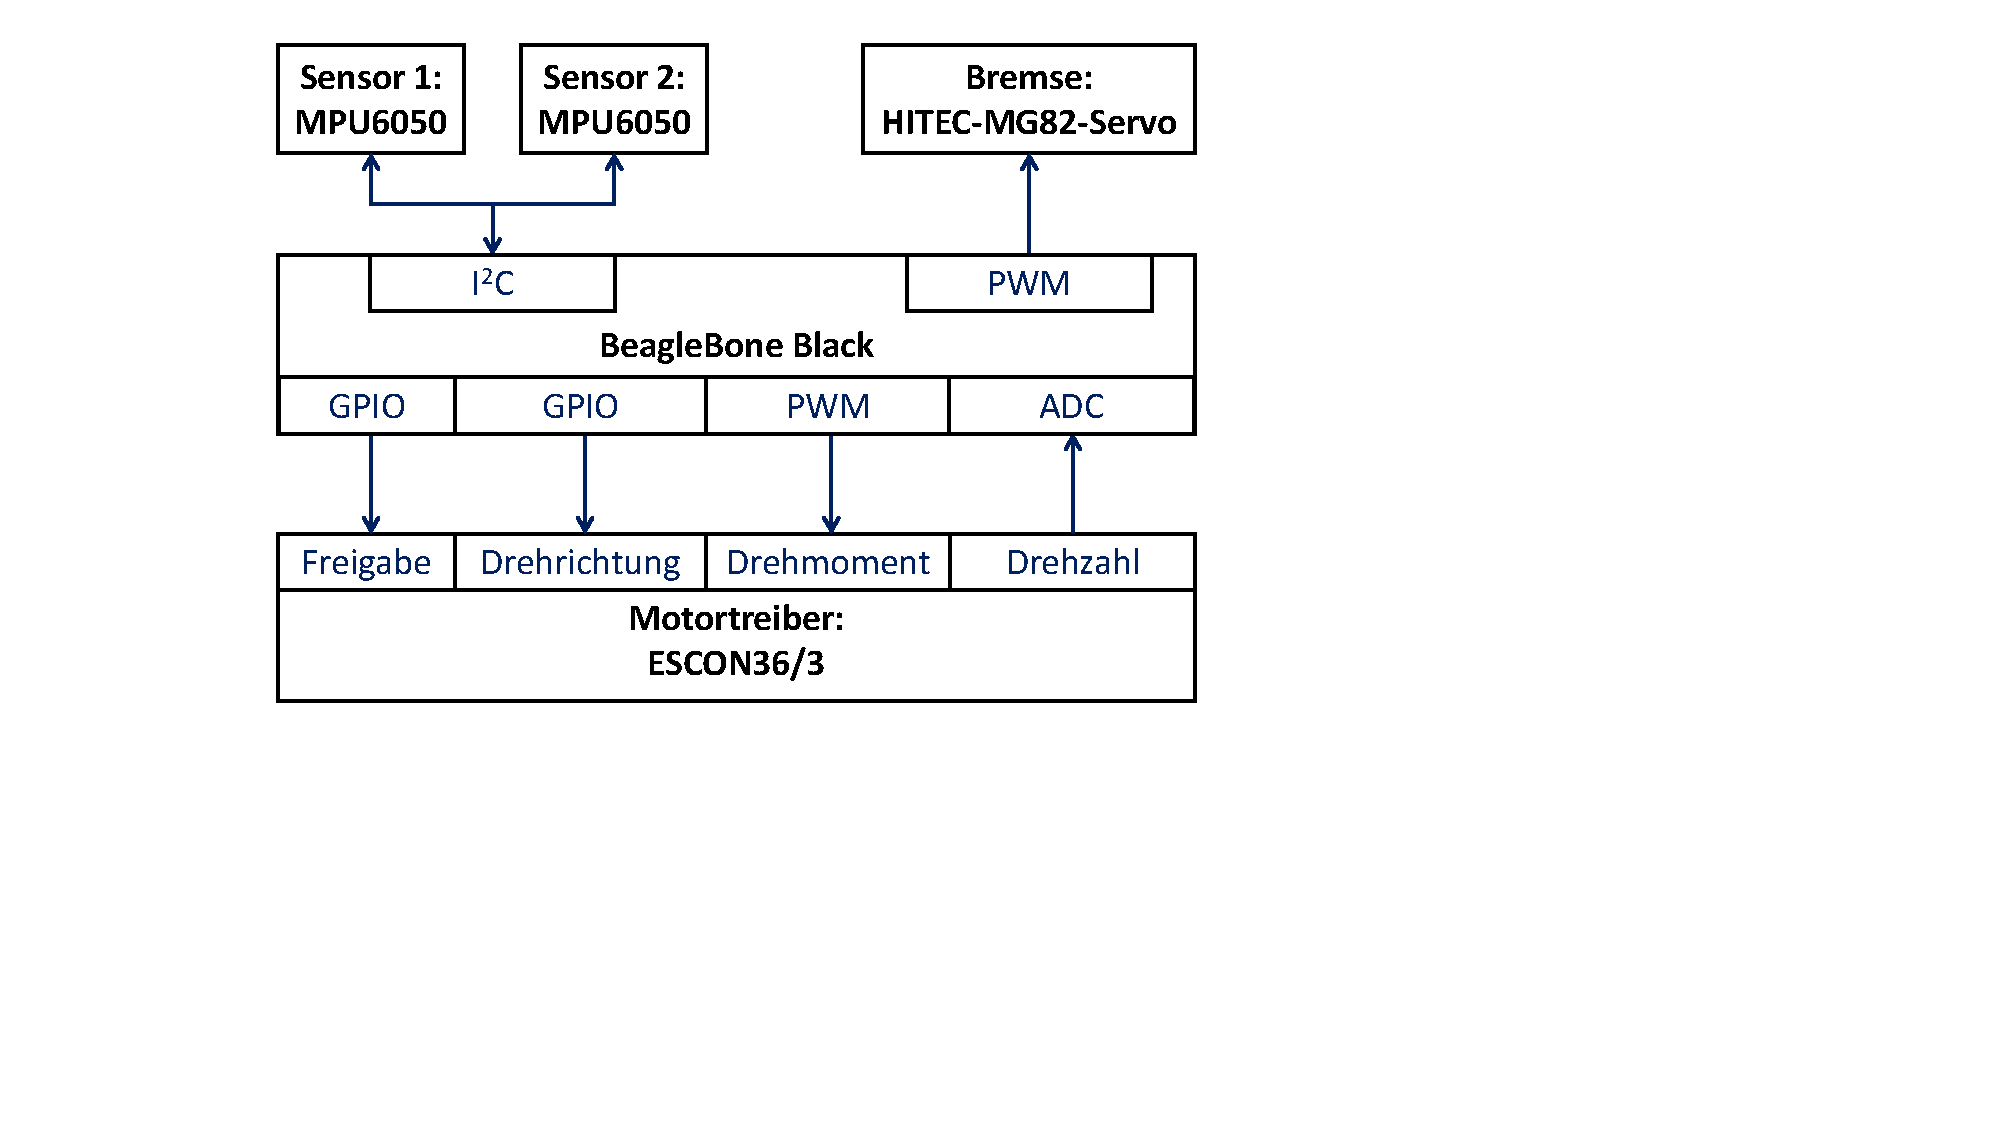
\includegraphics[width=0.7\linewidth, trim={2cm 7cm 11cm 0cm},clip]{img/ElekAufbau_Bauteile}
\caption{Übersicht Elektrik, Quelle: eigene Darstellung}

\end{figure}
\subsection{Konstruktion 1D}
Im Fokus der Konstruktionsansätze stand es, einen möglichst einfachen Aufbau zu entwickeln, der mit konventionellen Maschinen unter geringstem Einsatz fertigbar ist. Dies wurde durch die Verwendung von Standardmaterialien mit Standardmaßen erreicht, welche weit verbreitet sind. Weiter können alle Teile aus Blechen bzw. Stangenmaterial gefertigt werden, somit ist kein Einsatz von CNC Maschinen mit fünf oder mehr Achsen notwendig. In diesem Fall wurden 80 Prozent der Teile mittels einer Wasserstrahlschneidmaschine gefertigt. Der Einsatz von Passungen wurde auf das nötige Minimum reduziert. Aufgrund der Weiterverwendung dieses Projektes für eine Vorlesung, musste bei der Entwicklung darauf geachtet werden, das System möglichst wartungsfreundlich zu gestalten. Das gesamte Modell lässt sich in drei Baugruppen zerlegen, somit können alle Verschleißteile, wie z.B. Bremsbeläge und Lager schnell gewechselt werden. Aus Gewichtsgründen wurden alle Bauteile sehr schlank dimensioniert. 


\subsubsection{Bauteile}

Beim Bremsen drückt der Bremshebel auf die Schwungscheibe und presst diese gegen den unteren Bremsbelag. Dabei wird der Motorschaft radial belastet. Um diese Belastung zu verringern wird die Schwungmasse zusätzlich gelagert. Dies wird durch den Flansch mit Achse realisiert. In der Würfelseite ist ein Lager eingelassen, in dem die Achse des Flanschs geführt wird. 

	\begin{figure}[!h]
	\begin{center}
	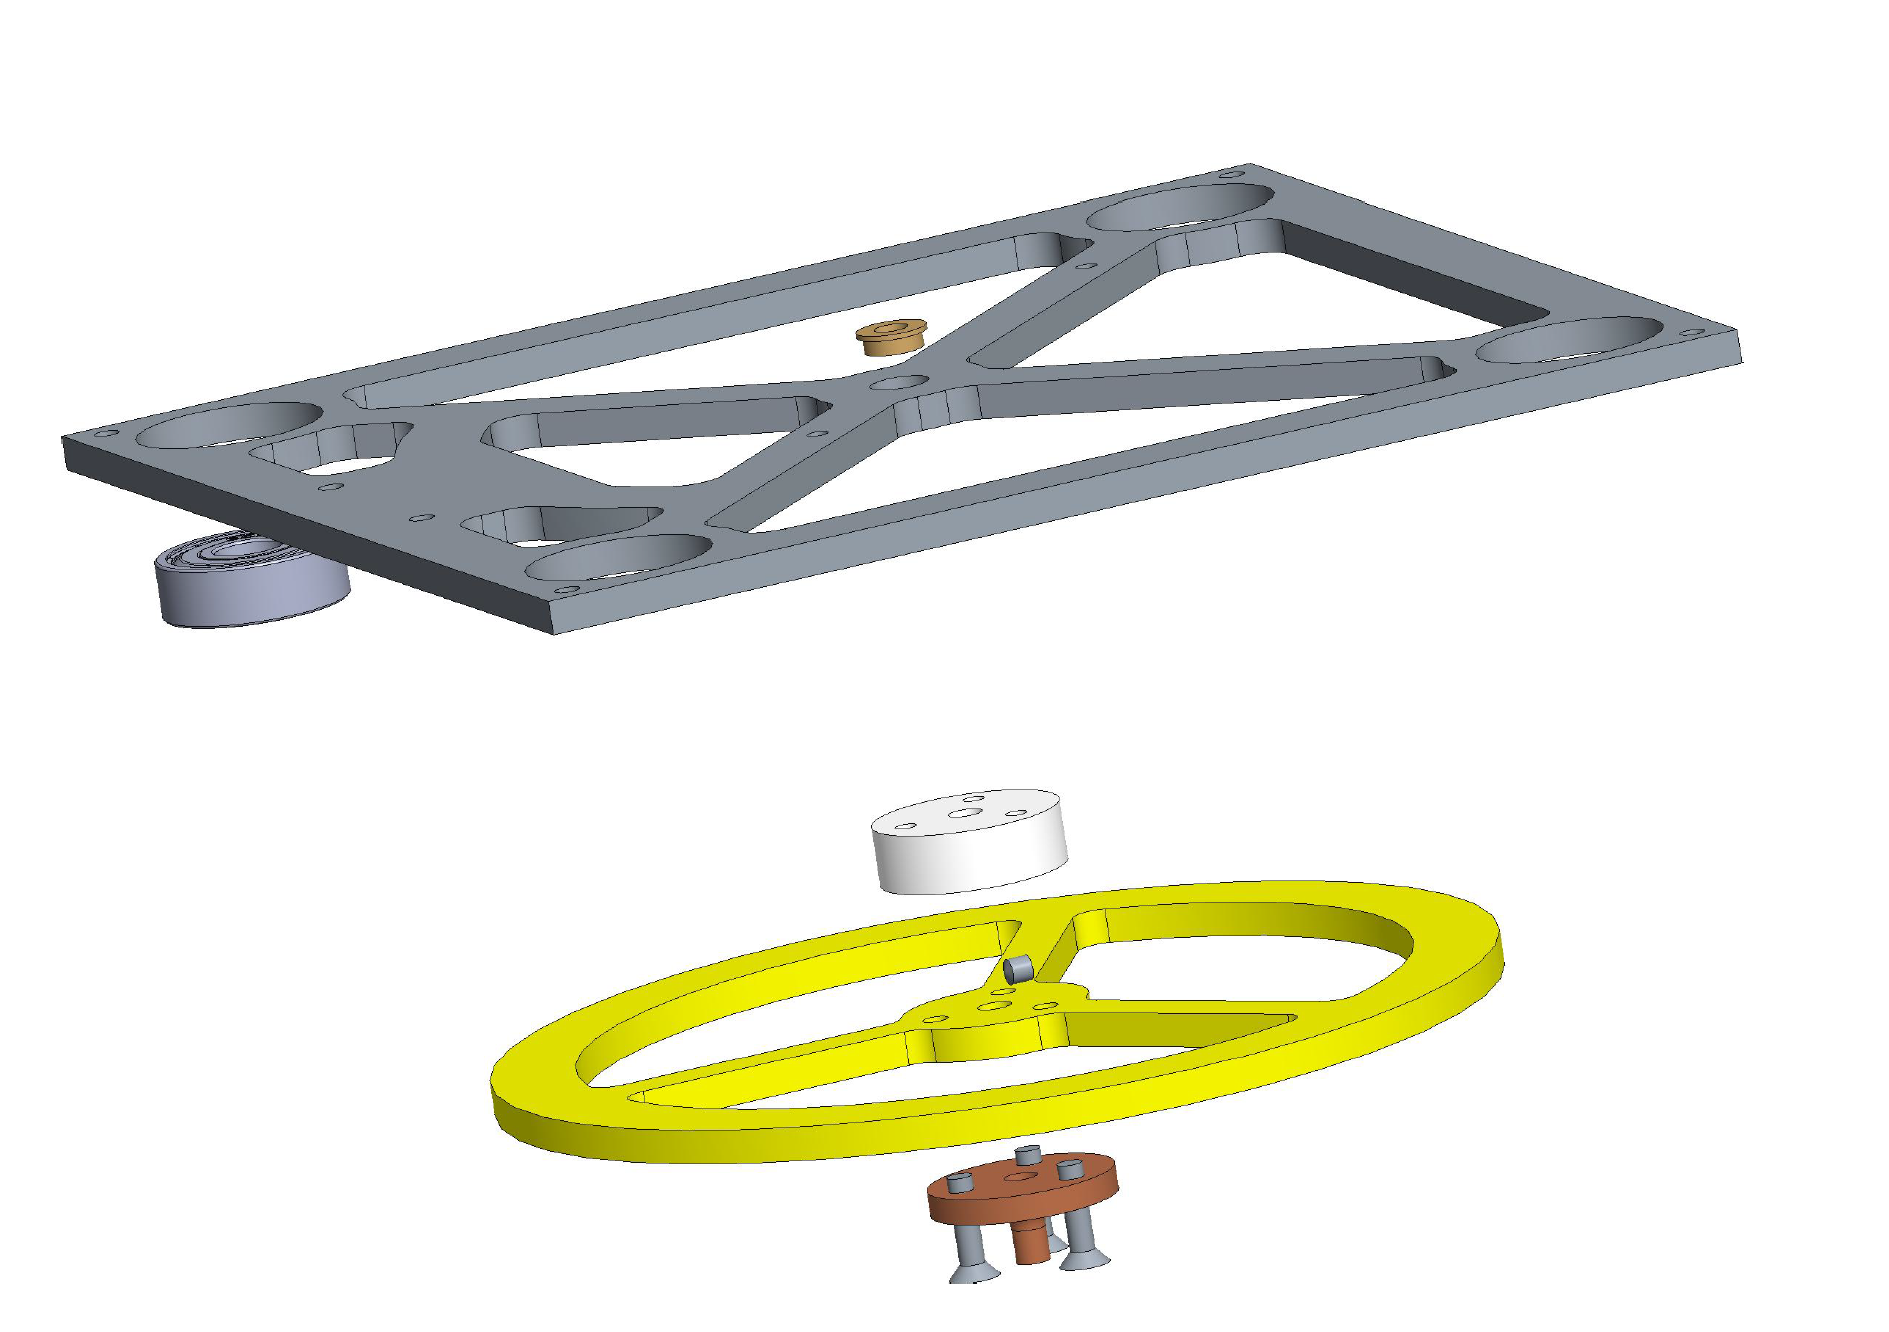
\includegraphics[width=0.75\textwidth]{img/Explosionszeichnung_Schwungscheibe.png}
	\end{center}
	\caption{Flansch Motorseite, Quelle: eigene Darstellung}
	\end{figure} 
 

	\begin{figure}[!h]
	\begin{center}
	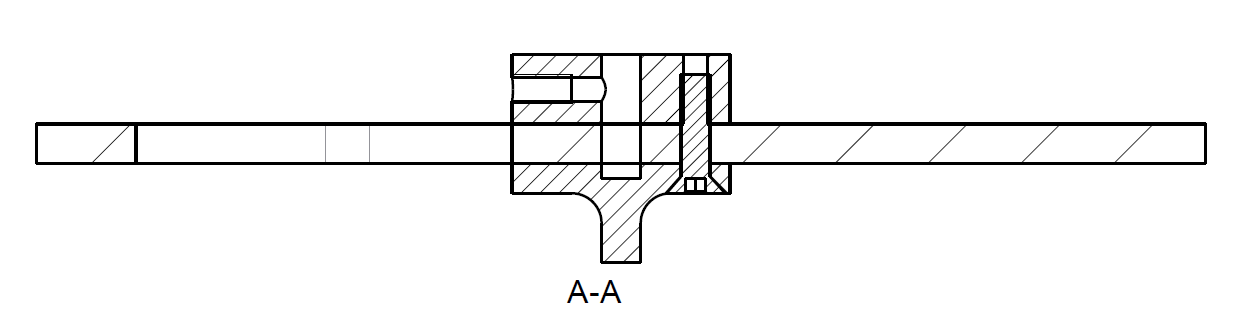
\includegraphics[width=0.75\textwidth]{img/Schwungmasse_mit_Flanschen_Schnitt}
	\end{center}
	\caption{Schnitt durch Schwungmasse mit beiden Flanschen, Quelle: eigene Darstellung}
	\end{figure} 

Der Motor selbst wird auf dem Motorhalter befestigt, welcher wiederum über die Halteplatte mit der Würfelseite verbunden ist. Am Motorhalter ist zusätzlich der Servo-Motor befestigt, der für die Aktuierung der Bremse notwendig ist. 
Im Hinblick auf die Konstruktion des gesamten Würfels, muss der Motorhalter zusätlich angepasst werden, so dass die Befestigung des Motors in zwei Richtungen erfolgen kann. Im Würfel würden drei gleiche Motorhalter dazu führen, dass die Bauteile sich gegenseitig im Weg stehen. 

	\begin{figure}[h!]
	\begin{center}
	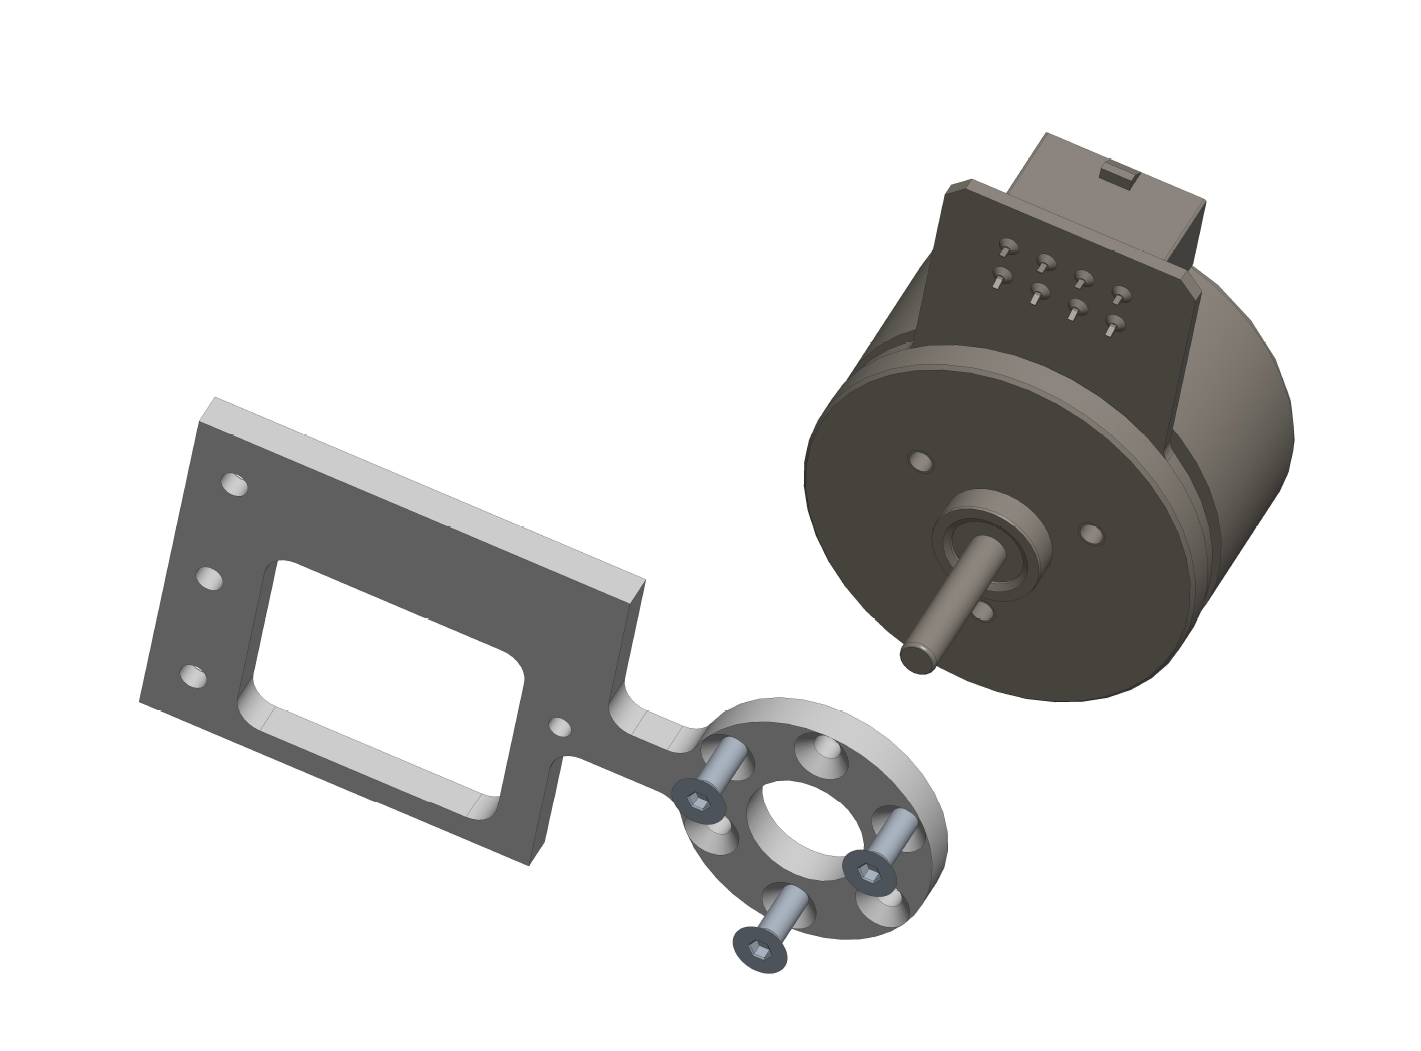
\includegraphics[width=0.75\textwidth]{img/Explosionszeichnung_Motor_Motorhalter.png}
	\end{center}
	\caption{Motorhalter, Quelle: eigene Darstellung}
	\end{figure} 

Die Bremse wird durch den Servo-Motor über das Servohorn nach dem Hebelprinzip bewegt. 


\begin{figure}[h!]
	\begin{center}
	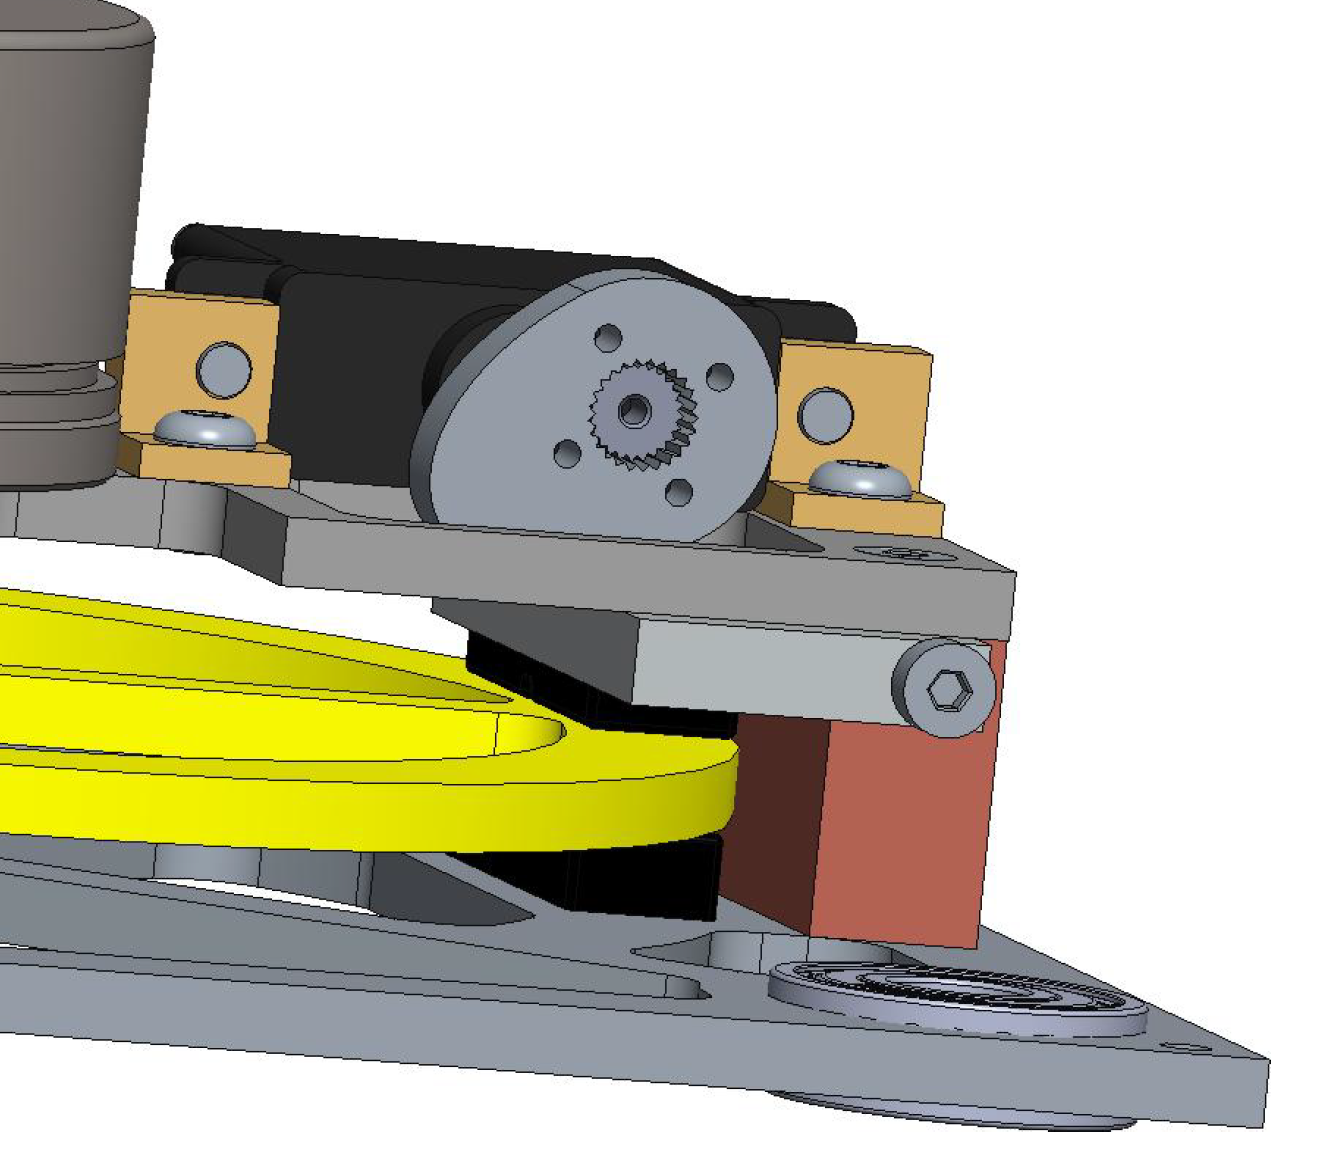
\includegraphics[width=0.75\textwidth]{img/Bremse_detail.png}
	\end{center}
	\caption{Bremsmechanismus, Quelle: eigene Darstellung}
	\end{figure} 

\newpage
Um die Komplexität des Systems vorerst zu vereinfachen, wurde diese Würfelseite zusammengebaut und in einer der Ecken gelagert um  Freiheitsgrade zu eliminieren. 
Die Bewegung kann somit nur noch in einer Ebene erfolgen. Von konstruktiver Seite wurden Aussparungen für ein 608ZZ-Lager vorgesehen. Über eine Achse, die fest gelagert wird, ergibt sich folgender Aufbau. 

\begin{figure}[h!]
	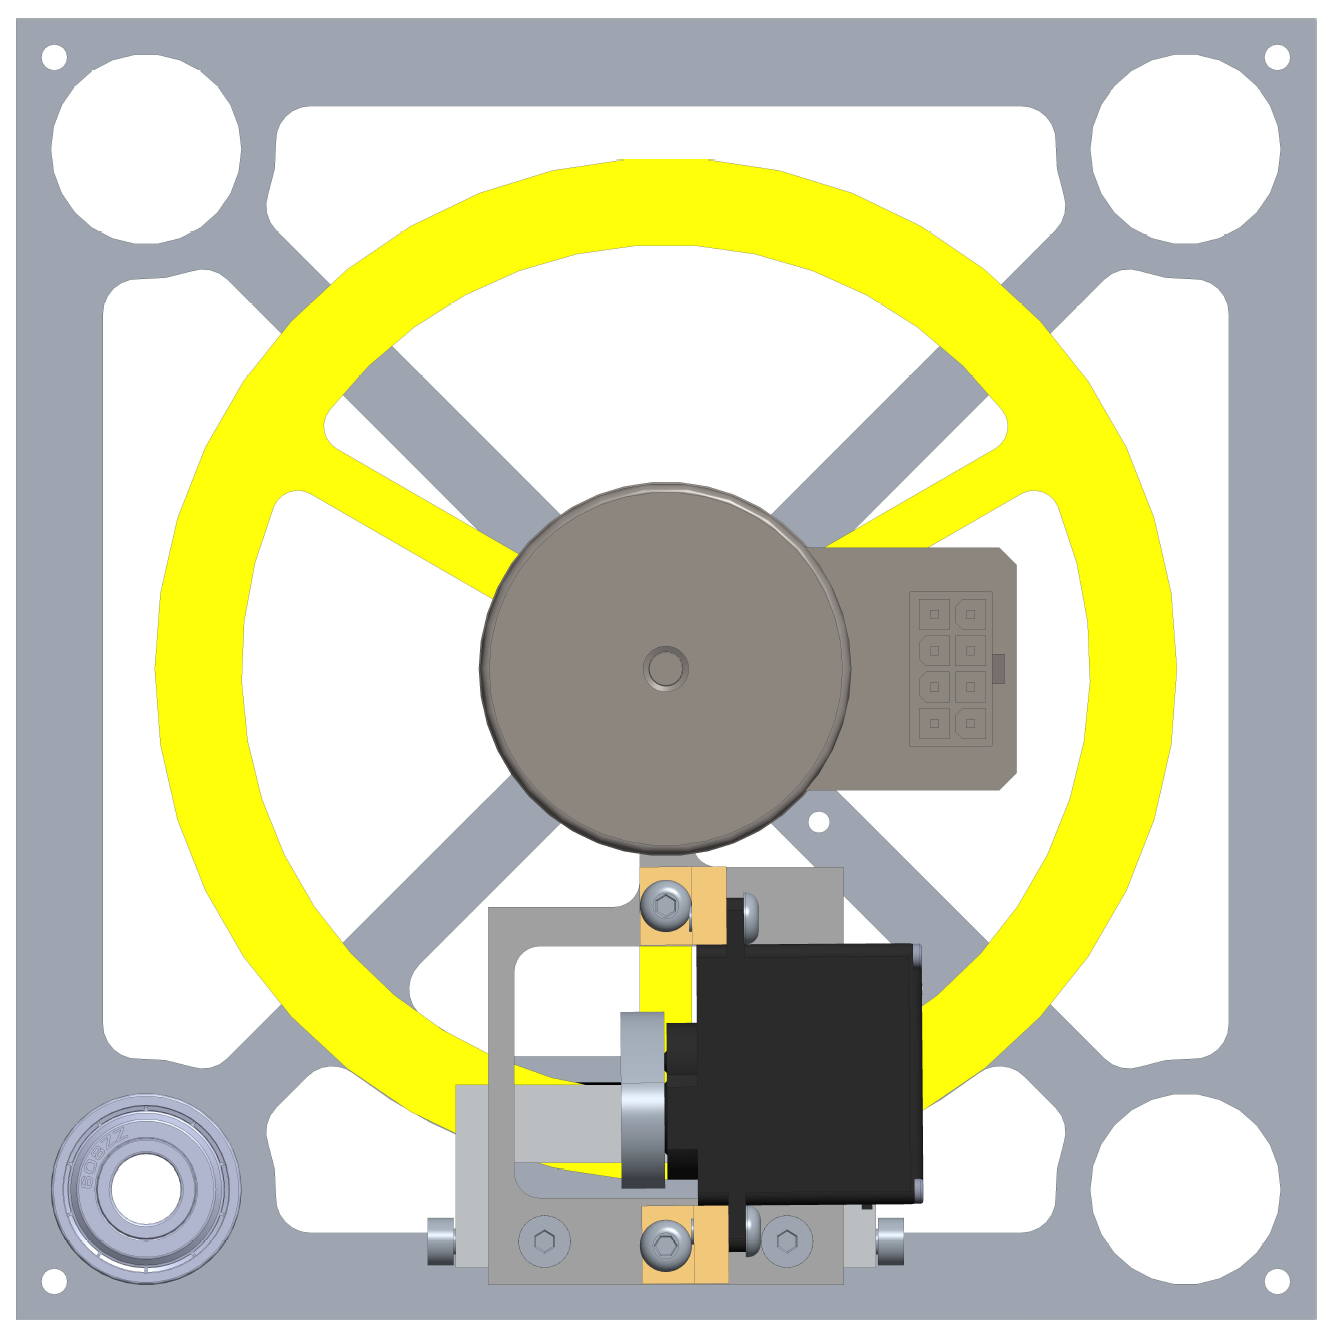
\includegraphics[width=0.49\textwidth]		  {img/1d_assembled_top}	   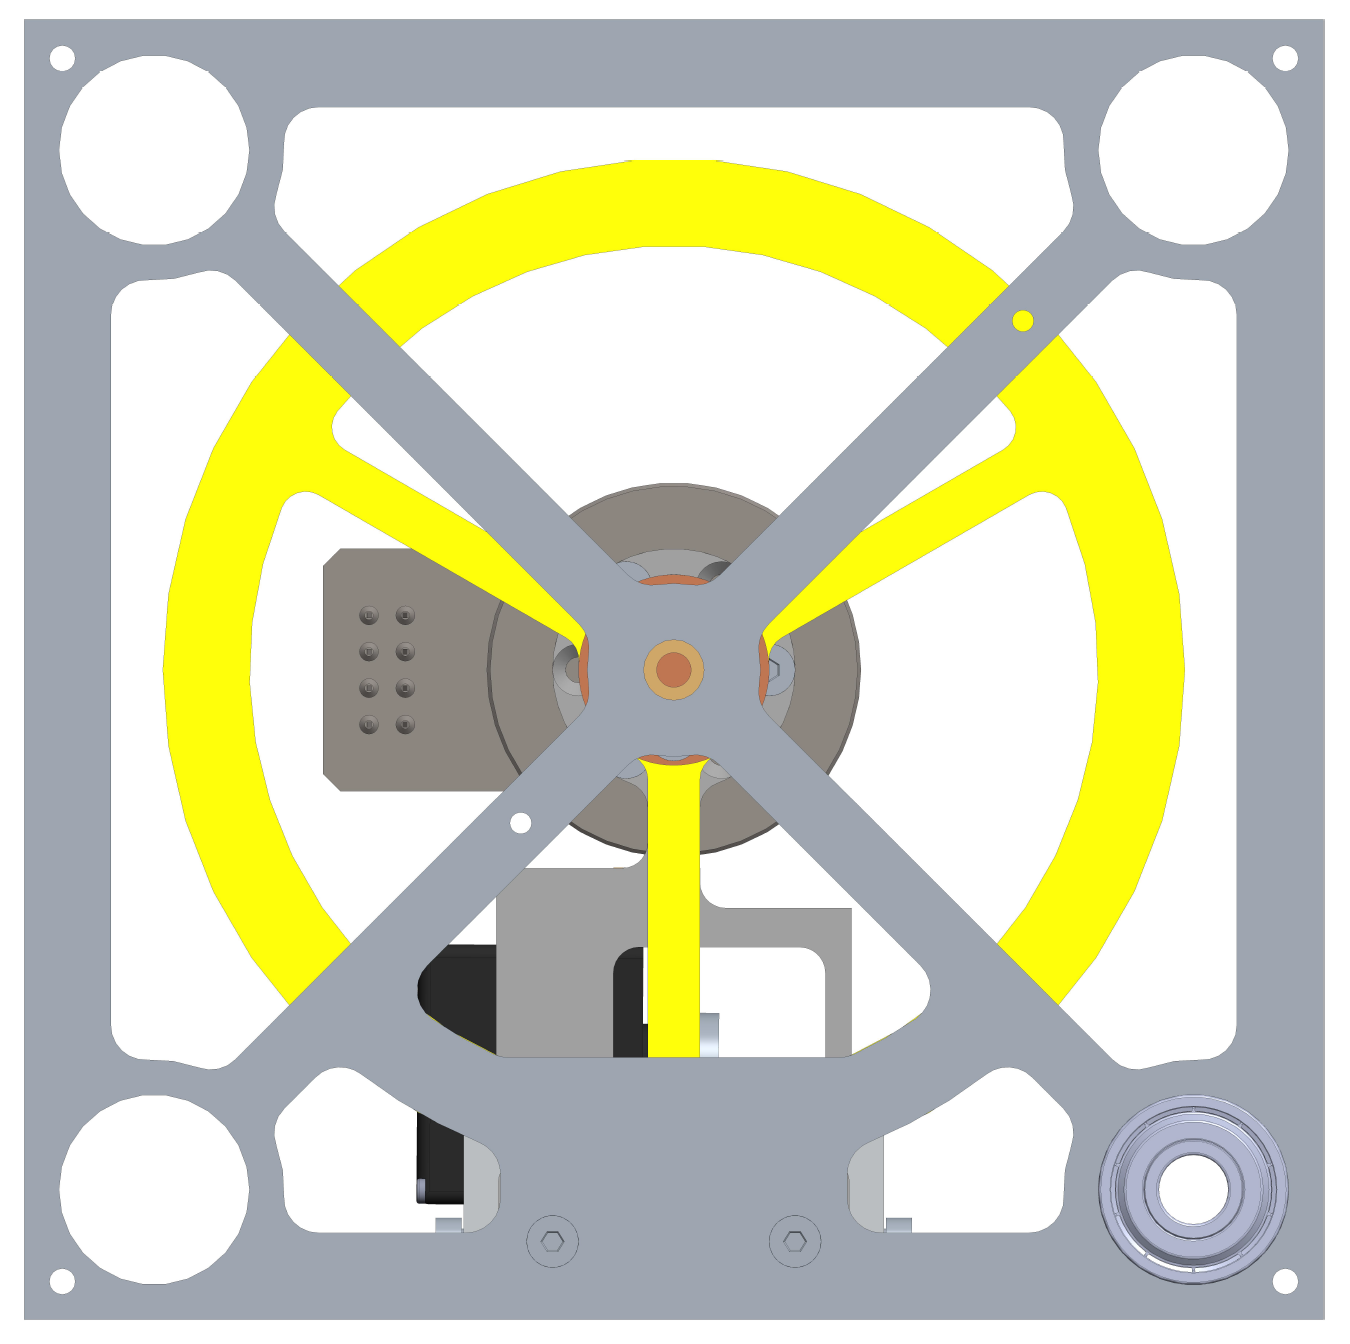
\includegraphics[width=0.49\textwidth]{img/1d_assembled_bottom}								\caption{Komplette Baugruppe, Quelle: eigene Darstellung} 
	\end{figure} 

\begin{figure}[h!]
	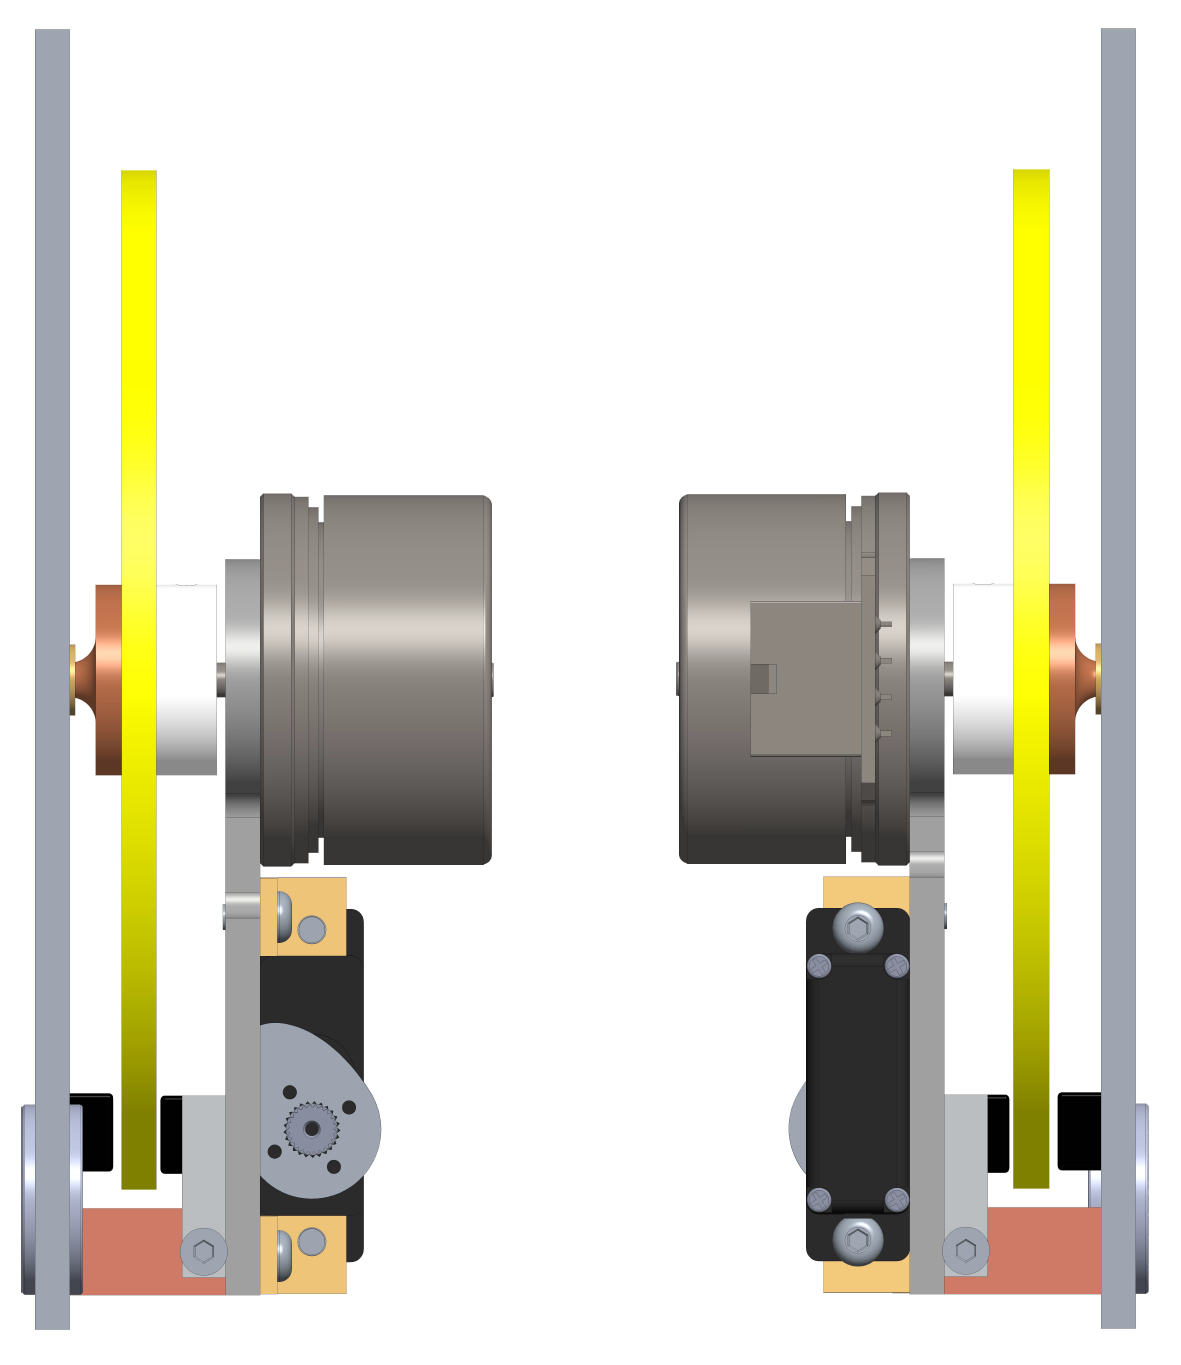
\includegraphics[width=0.49\textwidth]{img/1d_assembled_side}
	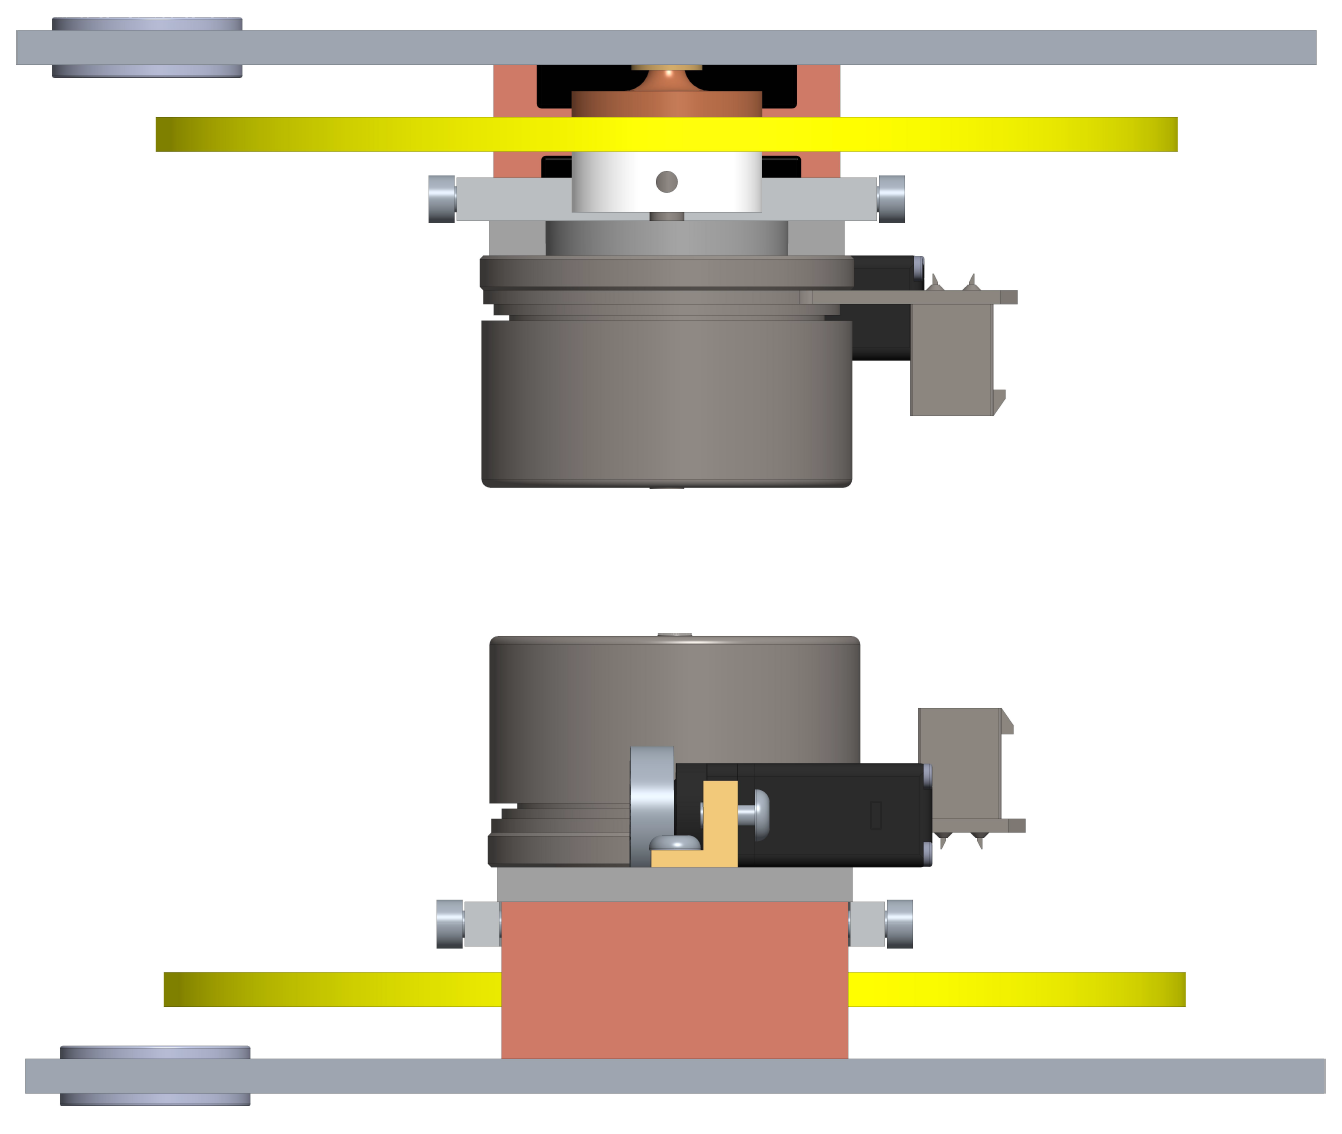
\includegraphics[width=0.49\textwidth]{img/1d_assembled_front_back}
	\caption{Komplette Baugruppe, Quelle: eigene Darstellung} 
	\end{figure} 

	\begin{figure}[h!]
	\begin{center}
	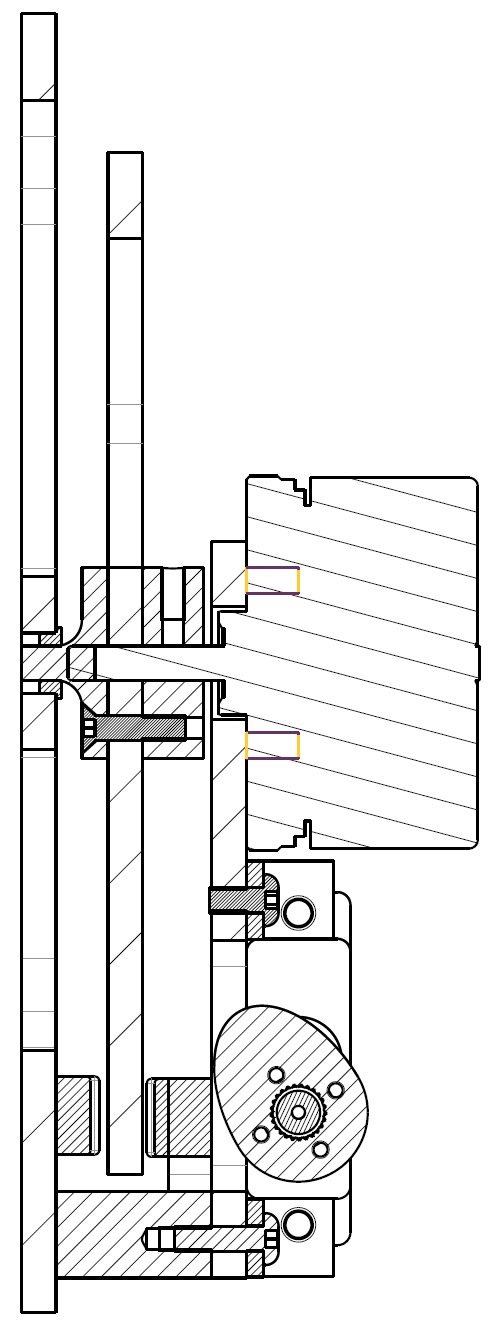
\includegraphics[width=0.4\textwidth,angle=90]{img/1d_assembled_schnitt}
	\end{center}
	\caption{Schnitt durch komplette Baugruppe, Quelle: eigene Darstellung}
	\end{figure} 
 

		

\subsection{Modellierung der Systemdynamik} \label{Dynamik_sec}
In dem folgenden Abschnitt werden die Bewegungsgleichungen mit Hilfe des Lagrange Formalismus hergeleitet. Aus diesen Gleichung kann im Anschluss eine Zustandsraumdarstellung aufgestellt werden, welche als Grundlage für den Reglerentwurf dient.

\begin{figure}[h]
\centering
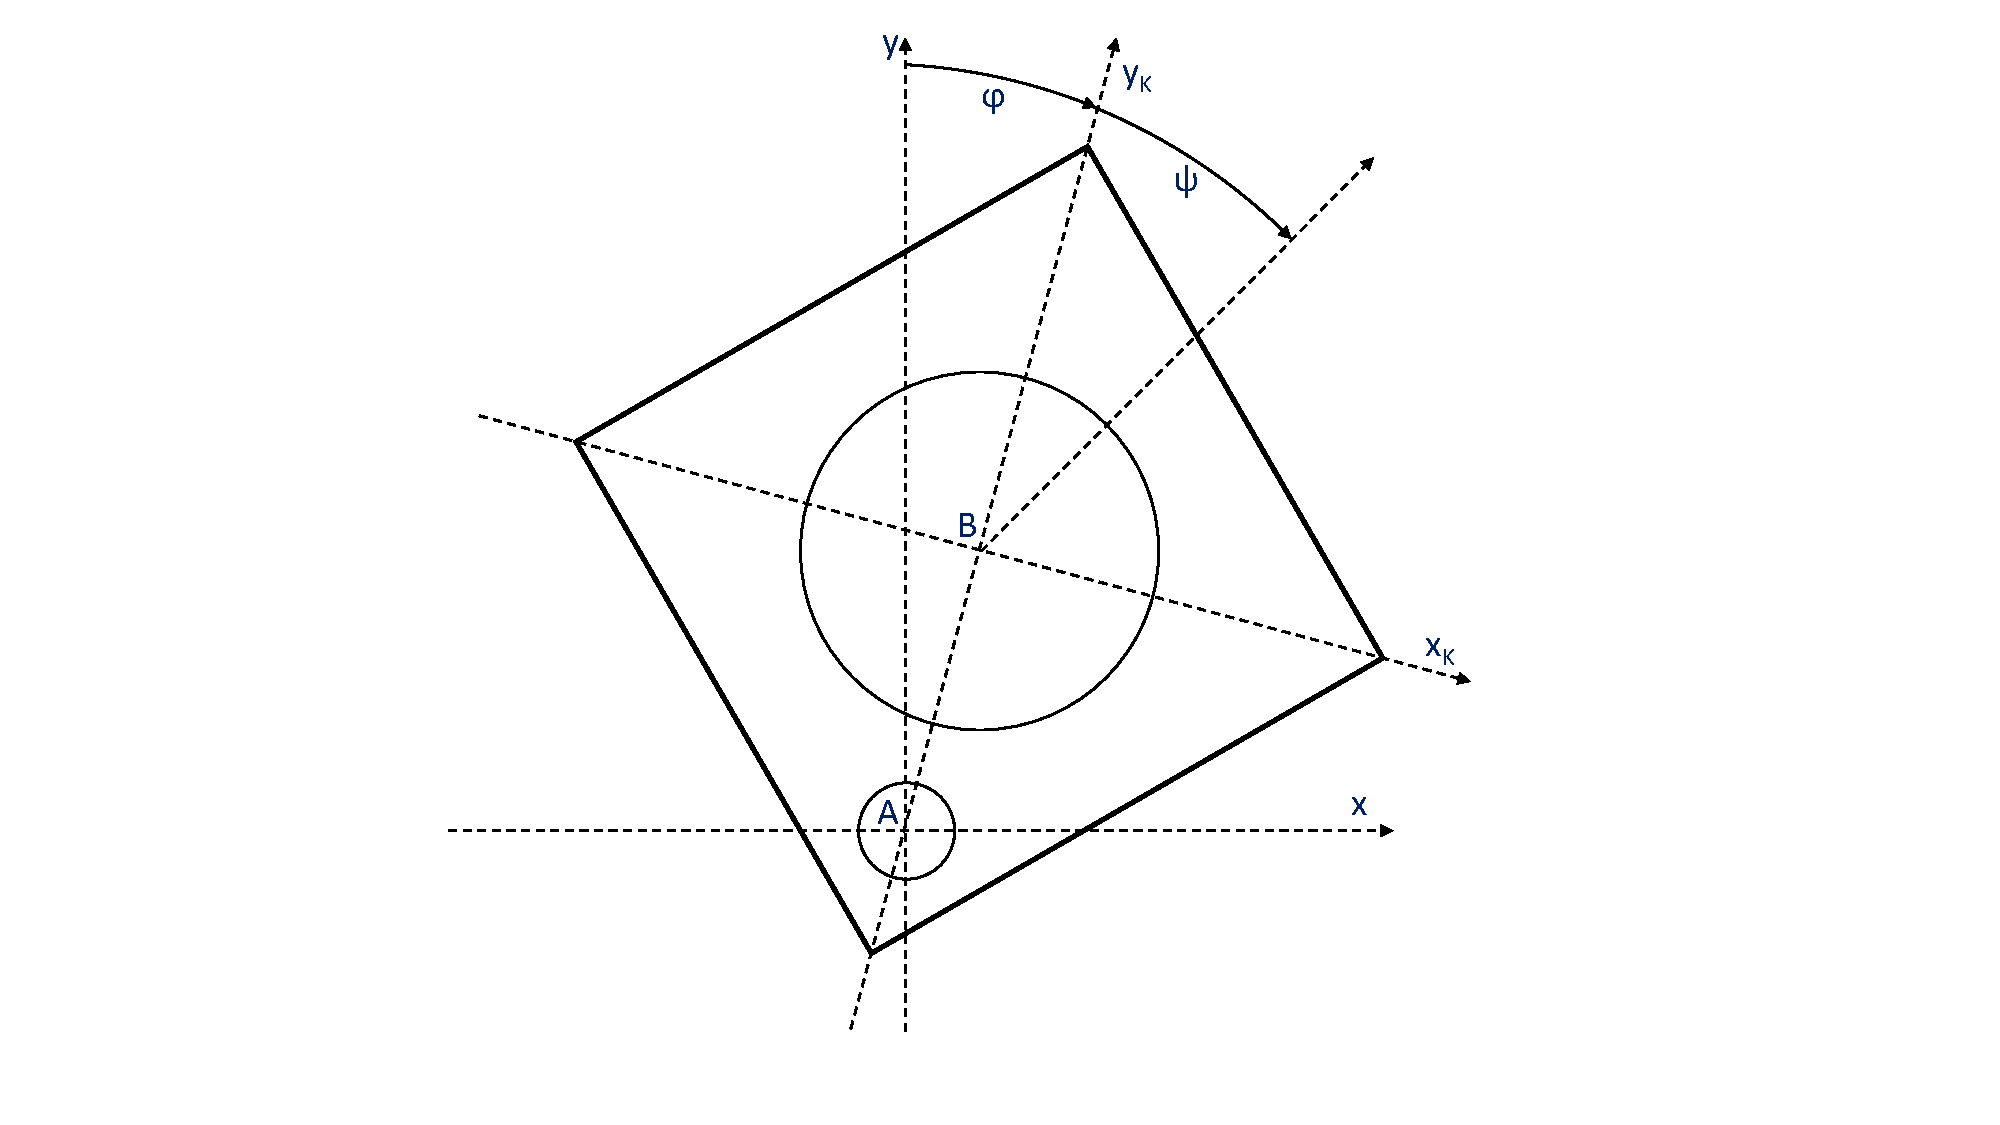
\includegraphics[width=\linewidth]{MechZeichnung1D}
\caption{Mechanischer Aufbau, Quelle: eigene Darstellung}
\end{figure}

Der Prototyp besteht aus einem starren Körper der in $A$ auf einer Achse gelagert ist. In $B$ ist eine Schwungmasse über einen Motor mit dem Körper verbunden. Somit verfügt das Gesamtsystem über zwei Freiheitsgrade, welche durch die generalisierten Koordinaten 

\begin{equation}
q_1 = \varphi \hspace{35pt} q_2 = \psi
\end{equation}

beschrieben werden. Der Winkel $\varphi$ wird von den Achsen $y$ und $y_K$ eingeschlossen. Der Winkel beschreibt die rotatorische Verschiebung der Schwungmasse zu dem Körper. Die folgenden Größen beschreiben die weiteren physikalischen Gegebenheiten des Systems.\newline

\begin{table}[h]
\centering
\begin{tabular}{|c|c|}
\hline
	\textbf{Variable} & \textbf{Erklärung} \\ \hline
	$q_1 = \varphi$ & Ausfallwinkel des Körpers \\ \hline
	$q_2 = \psi$ & Winkel zwischen Schwungmasse und Körper \\ \hline
	$A$ & Drehpunkt des Körpers \\ \hline
	$B$ & Drehpunkt des Schwungrades \\ \hline
	$l_{AB}$ & Abstand zwischen $A$ und $B$ \\ \hline
	$l_{AC}$ & Abstand zwischen $A$ und dem Schwerpunkt des Körpers \\ \hline
	$m_K$ & Masse des Körpers \\ \hline
	$m_R$ & Masse des Schwungrades \\ \hline
	${\theta}^A_K$ & Massenträgheitsmoment des Körper um $A$ \\ \hline
	${\theta}^B_R$ & Massenträgheitsmoment der Schwungmasse um $B$ \\ \hline
	$C_{\varphi}$ & Dynamischer Reibkoeffizient des Körpers in $A$ \\ \hline
	$C_{\psi}$ & Dynamischer Reibkoeffizient des Schwungrades in $B$ \\ \hline
	$T_M$ & Drehmoment des Motor \\ \hline
\end{tabular}
\end{table}

\newpage
Um die Bewegungsgleichungen des Systems zu ermitteln wird der Lagrange Formalismus verwendet. Dieser basiert auf der Lagrange-Funktion $L$, welche die Differenz der kinetischen Energie $T$ und der potenziellen Energie $V$ des Systems beschreibt.

\begin{equation}
T = \frac{1}{2}[({\theta}^A_K + m_R \cdot {l_{AB}}^2) {\dot{\varphi}}^2 + {\theta}^R_B(\dot{\varphi}+\dot{\psi})^2]
\end{equation}
\begin{equation}
V = g(m_R \cdot l_{AB} + m_K \cdot l_{AC})cos(\varphi)
\end{equation}
\begin{equation}
L = T - V = \frac{1}{2}[({\theta}^A_K + m_R \cdot {l_{AB}}^2) {\dot{\varphi}}^2 + {\theta}^R_B(\dot{\varphi}+\dot{\psi})^2] - g(m_R \cdot l_{AB} + m_K \cdot l_{AC})cos(\varphi)
\end{equation}

In dem System wirken unterschiedliche Kräfte. Einerseits erzeugt der Motor ein Drehmoment, welches die virtuelle Arbeite $\delta W_M$ verursacht. Andererseits verrichtet die Gravitation die virtuelle Arbeite $\delta W_G$. Zusätzlich muss die, durch die Reibung entstandene, Verlustleistung berücksichtigt werden. In diesem Fall wird die Reibleistung mit den Rayleigh'schen Dissipationsfunktionen $D_{\varphi}$ und $D_{\psi}$ beschrieben und verrichten die virtuelle Arbeit $\delta W_D$.

\begin{equation}
-\delta W_M = T_M \cdot \delta \psi
\end{equation}

\begin{equation}
-\delta W_G = g(m_K \cdot l_{AC} + m_R \cdot l_{AB})sin(\varphi) \cdot \delta \varphi
\end{equation}

\begin{equation}
D_{\varphi} = \frac{1}{2}C_{\varphi} \cdot {\dot{\varphi}}^2
\end{equation}
\begin{equation}
D_{\psi} = \frac{1}{2}C_{\psi} \cdot {\dot{\psi}}^2
\end{equation}
\begin{equation}
D = D_{\varphi} + D_{\psi} = \frac{1}{2}C_{\varphi} \cdot {\dot{\varphi}}^2 + \frac{1}{2}C_{\psi} \cdot {\dot{\psi}}^2
\end{equation}
\begin{equation}
-\delta W_D = - C_{\varphi} \cdot \dot{\varphi} \cdot \delta \varphi - C_{\psi} \cdot \dot{\psi} \cdot \delta \psi
\end{equation}

Die Summe der virtuellen Arbeiten, welche von den verschiedenen Kräften verrichtet wird, ergibt die virtuelle Arbeit des Gesamtsystems $\delta W$. In dem die verrichtete Arbeit partiell nach den beiden generalisierten Koordinaten $\varphi$ und $\psi$ differenziert wird, können die beiden generalisierten Kraftkomponenten $Q_{\varphi}$ und $Q_{\psi}$ berechnet werden.

\begin{equation}
Q_{\varphi} = g(m_K \cdot l_{AC} + m_R \cdot l_{AB})sin(\varphi) - C_{\varphi} \cdot \dot{\varphi}
\end{equation}
\begin{equation}
Q_{\psi} = T_M - C_{\psi} \cdot \dot{\psi}
\end{equation}


Bei dem Prototyp handelt es sich um ein nicht konservatives System, da durch die Reibung mechanische Energie verloren geht und der Motor dem System mechanische Energie zuführt. Da die beiden generalisierten Koordinaten $\varphi$ und $\psi$ voneinander unabhängig sind können aus dem d'Alembert'schen Prinzip zwei Bewegungsgleichungen abgeleitet werden.

\begin{equation}
\frac{d}{dt}\frac{\partial T}{\partial \dot{q}_i}-\frac{\partial T}{\partial q_i} = Q_i
\end{equation}
\begin{equation}
\frac{d}{dt}\frac{\partial T}{\partial \dot{\varphi}}-\frac{\partial T}{\partial \varphi} = Q_{\varphi} 
\end{equation}
\begin{equation}
\label{LG_phi_equation}
({\theta}^A_K + {\theta}^B_R + m_R \cdot l_{AB}^2)\ddot{\varphi} + {\theta}^B_R \cdot \ddot{\psi} - g(m_R \cdot l_{AB} + m_K \cdot l_{AC})sin(\varphi) + C_{\psi} \cdot \dot{\psi} = 0
\end{equation}
\begin{equation}
\frac{d}{dt}\frac{\partial T}{\partial \dot{\psi}}-\frac{\partial T}{\partial \psi} + \frac{\partial T}{\partial \dot{\psi}} = Q_{\psi} 
\end{equation}
\begin{equation}
\label{LG_psi_euqation}
{\theta}^R_B \cdot \ddot{\psi} = T_M - C_{\psi} \cdot \dot{\psi} - {\theta}^B_R \cdot \ddot{\varphi}
\end{equation}

Durch Einsetzen von (\ref{LG_psi_euqation}) in (\ref{LG_phi_equation}) ergibt sich die folgende Bewegungsgleichung für die Würfelseite.

\begin{equation}
\label{BG_phi_quation}
\ddot{\varphi} = \frac{g(m_R \cdot l_{AB}^2 + m_K \cdot l_{AC})sin(\varphi) - C_{\varphi} \cdot \dot{\varphi} + C_{\psi} \cdot \dot{\psi} - T_M}{{\theta}^A_K + m_R \cdot l_{AB}^2}
\end{equation}

Die Bewegungsgleichung für die Schwungmasse ergibt sich durch Einsetzen von (\ref{BG_phi_quation}) in (\ref{LG_psi_euqation}).

\begin{equation}
\label{BG_psi_equation}
\ddot{\psi} = \frac{({\theta}^A_K + m_R \cdot l_{AB}^2 + {\theta}^B_R)(T_M - C_{\psi} \cdot \dot{\psi})}{({\theta}^A_K + m_R \cdot {l_{AB}}^2){\theta}^B_R} + \frac{C_{\varphi} \cdot \dot{\varphi} - g(m_R \cdot l_{AB} + m_K \cdot l_{AC})sin(\varphi)}{{\theta}^A_K + m_R \cdot {l_{AB}}^2}
\end{equation}
\subsection{Sensorik}
\label{Sensorik_sec}
Die Aufgabe der verwendeten Sensorik liegt darin die Werte für $\varphi$, und $\dot{\varphi}$ zu bestimmen. Hierfür wurden zwei MPU6050 ICs verwendet. Diese verfügen jeweils über einen Beschleunigungssensor und Gyroskop, welche Werte für drei Achsen ausgeben. Der Tiefpass der Sensoren wird auf eine Grenzfrequenz von $44Hz$ eingestellt, da hier einerseits eine erste Glättung der Daten erfolgt, andererseits aber keine zu große Verzögerung entsteht, welche sich wiederum negativ auf die Regelung auswirken könnte. Die Position und Ausrichtung der Sensoren ist in Abbildung \ref{Position_Sensoren_pic} dargestellt.

\begin{figure}[h]
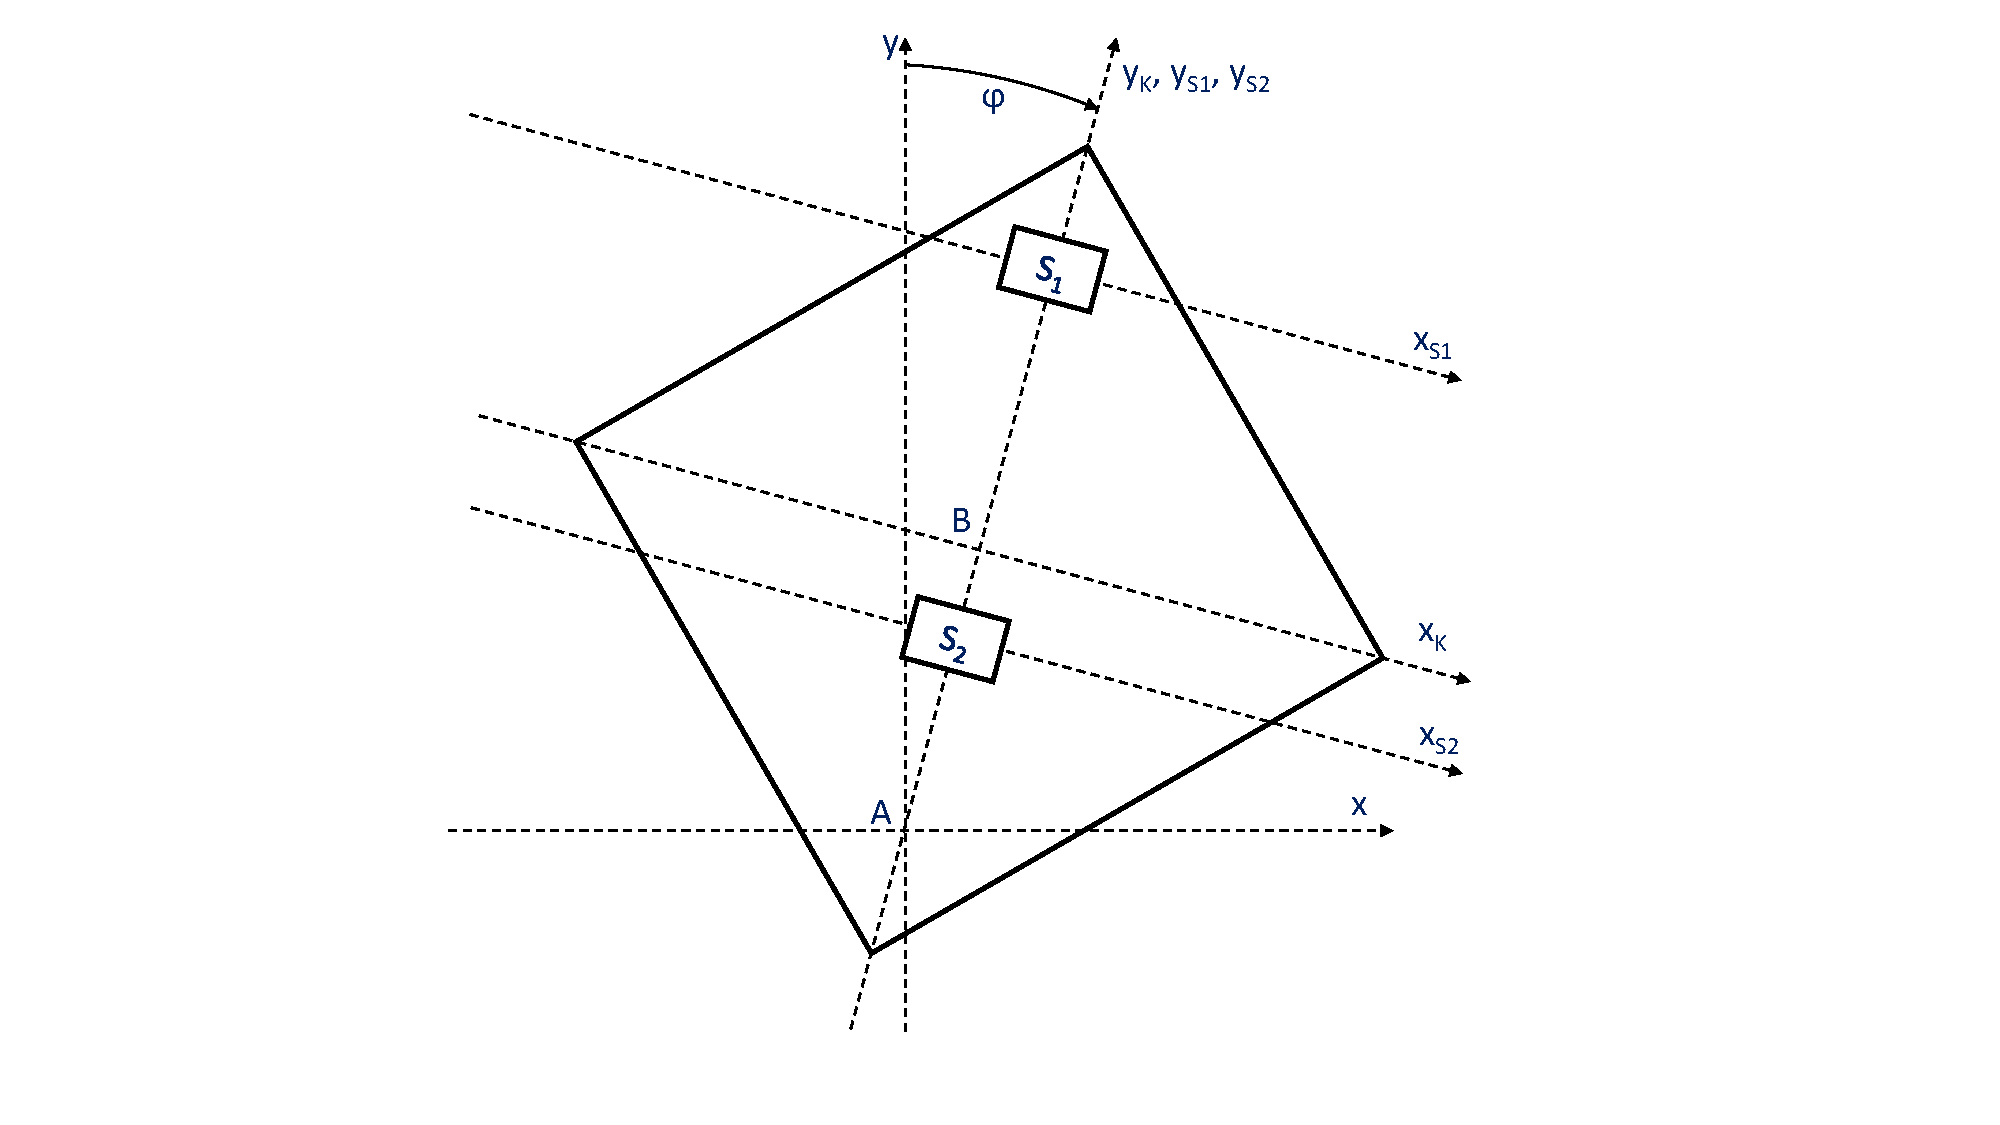
\includegraphics[width=\linewidth]{SensorZeichnung1D}
\caption{Position der Sensoren, Quelle: eigene Darstellung}

\label{Position_Sensoren_pic}
\end{figure}

\subsubsection{Winkelschätzung}
Die Sensoren sind nicht in der Lage Wege bzw. Winkel zu messen. Somit muss der Winkel $\varphi$ berechnet werden. Die gemessenen Beschleunigungen setzten sich aus einem statischen Anteil, welcher von $\varphi$ abhängt, und einem dynamischen Anteil, welcher von $\dot{\varphi}$ bzw. $\ddot{\varphi}$ abhängt, zusammen.

\begin{equation}
\ddot{S}_i = 
\begin{pmatrix}
\ddot{x}_i \\ \ddot{y}_i \\ \ddot{z}_i
\end{pmatrix} =
\begin{pmatrix}
r_{Si} \cdot \ddot{\varphi} + sin(\varphi) \cdot g \\
- r_{Si} \cdot \dot{\varphi}^2 - cos(\varphi) \cdot g \\
0
\end{pmatrix}
\hspace{35pt}
i \in [1;2]
\end{equation}

Da die dynamischen Anteile zusätzlich von dem Abstand $r_{Si}$ abhängen, kann die geometrische Anordnung der beiden Sensoren genutzt werden um das Verhältnis der beiden Anteile zu berechnen. Somit kann der aktuelle Wert von $\varphi$ nach \cite{Cubli1D} wie folgt berechnen.
\begin{equation}
\alpha = \frac{r_{S1}}{r_{S2}}
\end{equation}

\begin{equation}
\ddot{x}_1 - \alpha \cdot \ddot{x}_2 = 
g(1 - \alpha)sin(\varphi)
\end{equation}
\begin{equation}
\ddot{y}_1 - \alpha \cdot \ddot{y}_2 = 
-g(1- \alpha)cos(\varphi)
\end{equation}

\begin{equation}
\frac{\ddot{x}_1 - \alpha \cdot \ddot{x}_2}{\ddot{y}_1 - \alpha \cdot \ddot{y}_2} = -tan(\varphi)
\end{equation}

Nach dem selben Prinzip kann auch die Winkelbeschleunigung $\ddot{\varphi}$ berechnet werden.
\begin{equation}
\ddot{x}_1 - \ddot{x}_2 = [r_{S1} \cdot \ddot{\varphi} + sin(\varphi) \cdot g] - [r_{S2} \cdot \ddot{\varphi} + sin(\varphi) \cdot g] = (r_{S1} - r_{S2}) \cdot \ddot{\varphi}
\end{equation}
\begin{equation}
\ddot{\varphi} = \frac{\ddot{x}_1 - \ddot{x}_2}{r_{S1} - r_{S2}}
\end{equation}

\subsubsection{Kalibrierung und Justierung}
Die Sensoren geben die Beschleunigungs- und Geschwindigkeitswerte als 16 Bit Werte im Zweierkomplement aus. Diese Rohwerte müssen mit Hilfe eines Ausgleichspolynoms in die jeweilige SI-Einheit umgerechnet werden. 

\subsubsubsection{Umrechnung der Beschleunigungswerte}
Um das Polynom zur Umrechnung der Beschleunigungswerte zu ermitteln werden sieben Messungen in den fixen Ausfallpositionen $\phi \in [-45, -30, -15, 0, 15, 30, 45]$ durchgeführt. Pro Position werden $m = 10000$ Messwerte aufgenommen. Da in der Ruhelage die Beschleunigung lediglich von dem aktuellen Ausfallwinkel abhängt ist der Sollwert für jede Position bekannt. Somit kann ein Polynom erster Ordnung approximiert werden um Mittelwerte der sieben Positionen in die entsprechenden Beschleunigungswerte umzurechnen.

\begin{table}[h]
\centering
\begin{tabular}{lcllcl}
$\ddot{x}_n$ &$\equiv$& X-Beschleunigung Sensor n &
$\ddot{x}^R_n$ &$\equiv$& X-Rohwert Sensor n \\
$\ddot{y}_n$ &$\equiv$& Y-Beschleunigung Sensor n &
$\ddot{y}^R_n$ &$\equiv$& Y-Rohwert Sensor n
\end{tabular}
\end{table}

\vspace*{-\baselineskip}
\begin{equation}
\ddot{x}_n = p^1_{x_n} \cdot \ddot{x}^R_n + p^2_{x_n} \hspace{35pt} \vert \hspace{3pt} n \in \{1, 2\}
\end{equation}
\begin{equation}
\ddot{y}_n = p^1_{y_n} \cdot \ddot{y}^R_n + p^2_{y_n} \hspace{35pt} \vert \hspace{3pt} n \in \{1, 2\}
\end{equation}
\vspace*{-\baselineskip}
\begin{table}[h]
\centering
\begin{tabular}{lcllcl}
$p^1_{x_1}$ &$=$& $-5.992 \cdot 10^{-4}$ & $p^2_{x_1}$ &$=$& $0.3328$ \\
$p^1_{x_2}$ &$=$& $-6.003 \cdot 10^{-4}$ & $p^2_{x_2}$ &$=$& $0.4138$ \\
$p^1_{y_1}$ &$=$& $-6.127 \cdot 10^{-4}$ & $p^2_{y_1}$ &$=$& $0.1186$ \\
$p^1_{y_2}$ &$=$& $-6.81 \cdot 10^{-4}$ & $p^2_{y_2}$ &$=$& $0.1143$ \\
\end{tabular}
\end{table}

\vspace*{-\baselineskip}
\begin{figure}[h]
	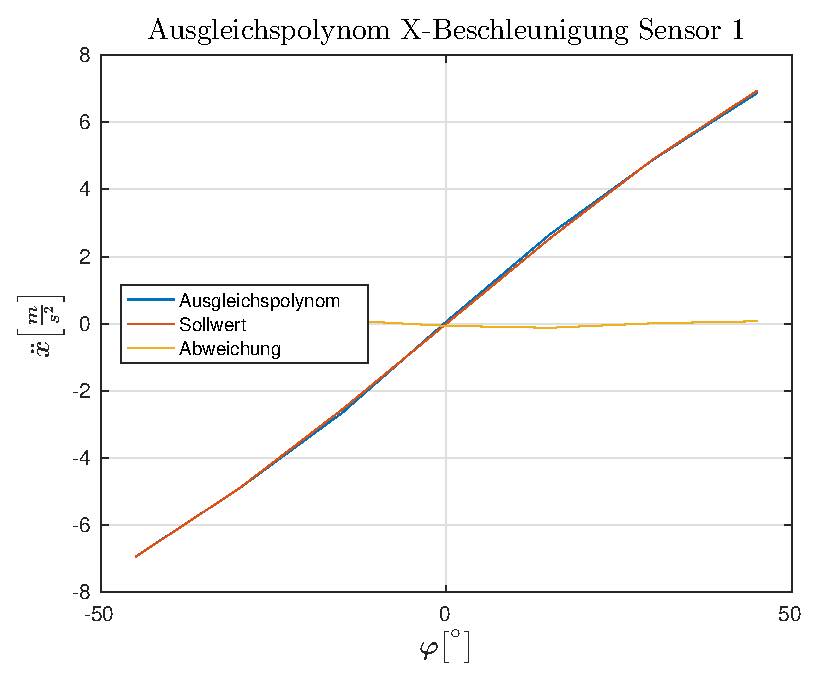
\includegraphics[width=0.5\linewidth]{img/X1__dd___fitted.eps}
	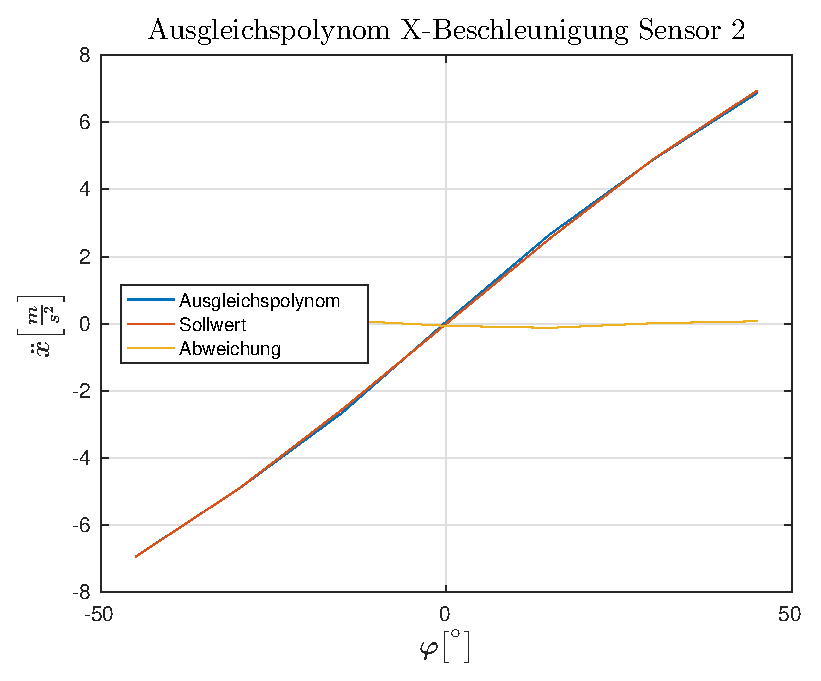
\includegraphics[width=0.5\linewidth]{img/X2__dd___fitted.eps}
\end{figure}

\vspace*{-\baselineskip}
\begin{figure}[h!]
	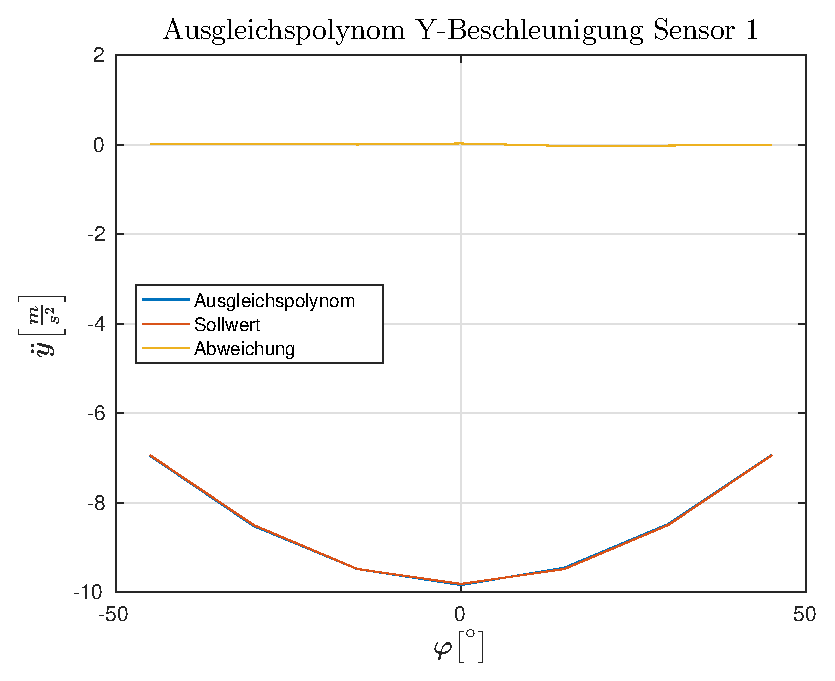
\includegraphics[width=0.5\linewidth]{img/Y1__dd___fitted.eps}
	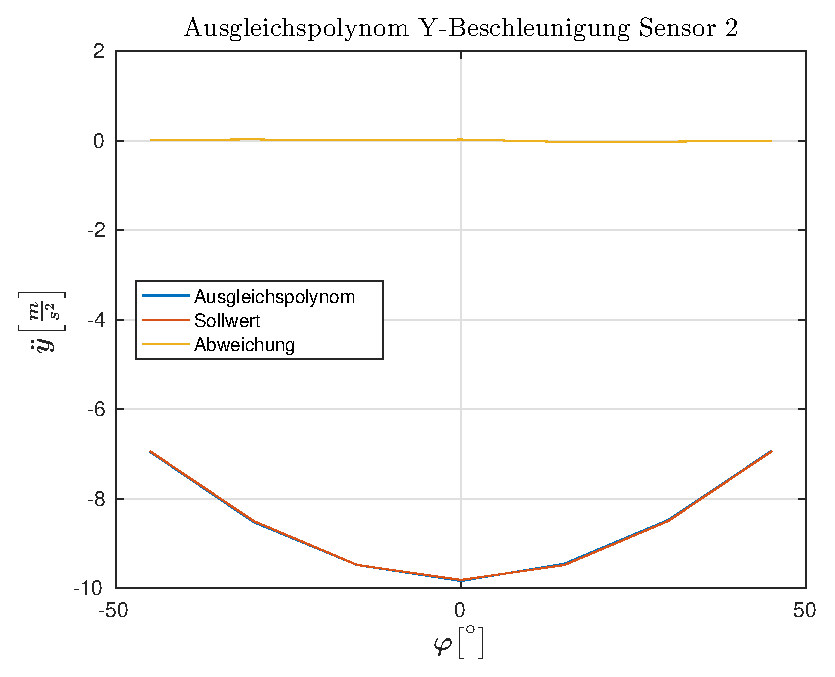
\includegraphics[width=0.5\linewidth]{img/Y2__dd___fitted.eps}
\end{figure}

\subsubsubsection{Umrechnung der Winkelgeschwindigkeiten}
Um die Rohwerte der Gyroskope in Winkelgeschwindigkeiten umzurechnen wird die Würfelseite fixiert und die Winkelgeschwindigkeitswerte der beiden Sensoren aufgenommen. Hierbei werden jeweils $m = 1000$ Werte aufgenommen. Da der Sollwert $\dot{\varphi} = 0 \frac{m}{s}$ bekannt ist kann die systematische Messabweichung der Sensoren über den Mittelwert bestimmt werden. Der proportionale Umrechnungsfaktor von Rohdaten zu Winkelgeschwindigkeiten wird dem Datenblatt des Herstellers entnommen.
\begin{figure}[h]
	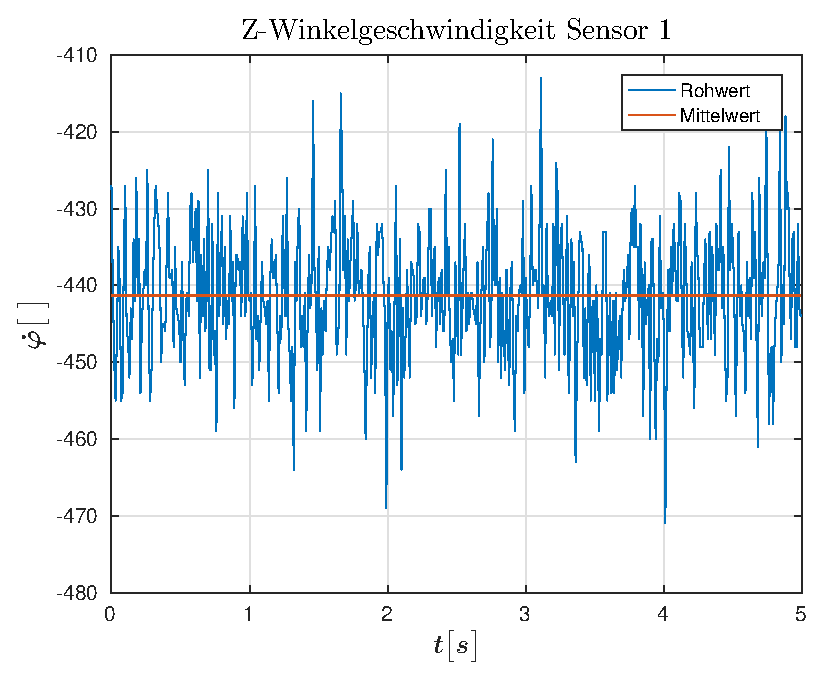
\includegraphics[width=0.5\linewidth]{img/phi1__d.eps}
	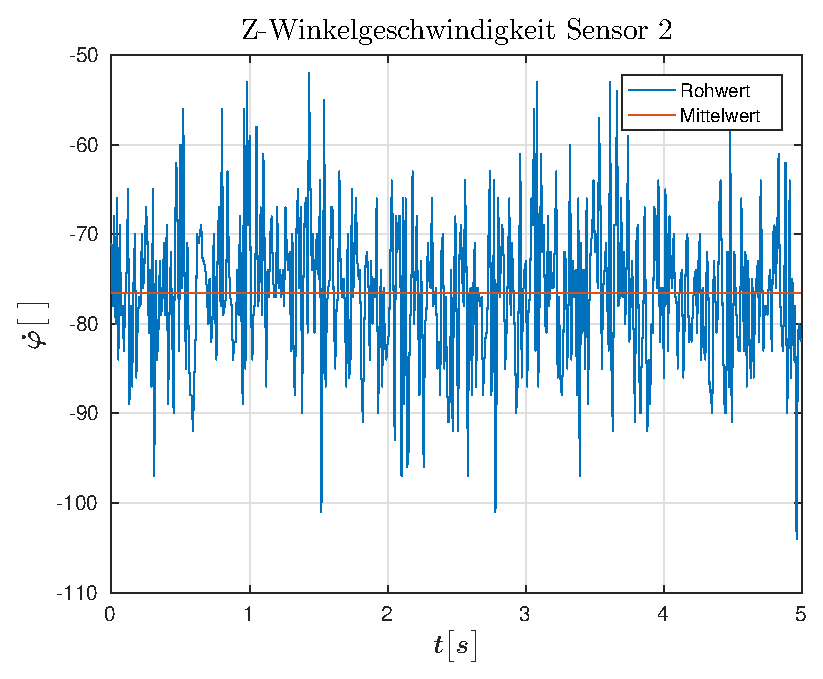
\includegraphics[width=0.5\linewidth]{img/phi2__d.eps}
\end{figure}
\vspace*{-\baselineskip}
\begin{table}[h]
\centering
\begin{tabular}{lcllcl}
$\dot{\varphi}_n$ & $\equiv$ & $\varphi$-Geschwindigkeit Sensor n & $\dot{\varphi}^R_n$ & $\equiv$ $\dot{\varphi}$-Rohwert Sensor n
\end{tabular}
\end{table}
\vspace*{-\baselineskip}
\begin{equation}
\dot{\varphi}_n = p^1_{\dot{\varphi}^R_n}  \cdot (\dot{\varphi}_n + p^2_{\dot{\varphi}_n})
\end{equation}
\vspace*{-\baselineskip}
\begin{table}[h]
\centering
\begin{tabular}{lcllcl}
$p^1_{\varphi_1}$ &$=$& $-1.3265 \cdot 10^{-4}$ & $p^2_{\varphi_1}$ &$=$& $441.3160$ \\
$p^1_{\varphi_2}$ &$=$& $-1.3265 \cdot 10^{-4}$ & $p^2_{\varphi_2}$ &$=$& $76.5140$ \\
\end{tabular}
\end{table}
\vspace*{-\baselineskip}
\subsubsection{Auswertung der Radgeschwindigkeit $\dot{\psi}$}
Der Motortreiber liefert ein analoges Spannungssignal, welches die aktuelle Motorgeschwindigkeit wiedergibt. Um die ADC-Werte in SI-Einheiten umzurechnen wird ein Polynom erster Ordnung benötigt. Hierfür werden mit Hilfe der ESCON-Studio-Anwendung konstante Motorgeschwindigkeiten ($\dot{\psi} \in \{ -3000, -2000,$  $-1000, 0, 1000, 2000, 3000 \} [rpm] $) gefahren und pro Durchlauf $m=500$ ADC-Werte aufgenommen. Über die Mittelwerte der Messungen und die vorgegebenen Radgeschwindigkeiten wird anschließend ein Polynom erster Ordnung approximiert.
\begin{table}[h!]
\centering
\begin{tabular}{lcllcl}
$\dot{\psi}$ & $\equiv$ & Geschwindigkeit der Schwungmasse & $\dot{\psi}_{ADC}$ & $\equiv$ & ADC-Wert
\end{tabular}
\end{table}
\vspace*{-\baselineskip}
\begin{equation}
\dot{\psi} = -0.5092 \cdot \dot{\psi}_{ADC} + 1050
\end{equation}
\vspace*{-\baselineskip}
\begin{figure}[h!]
\centering
	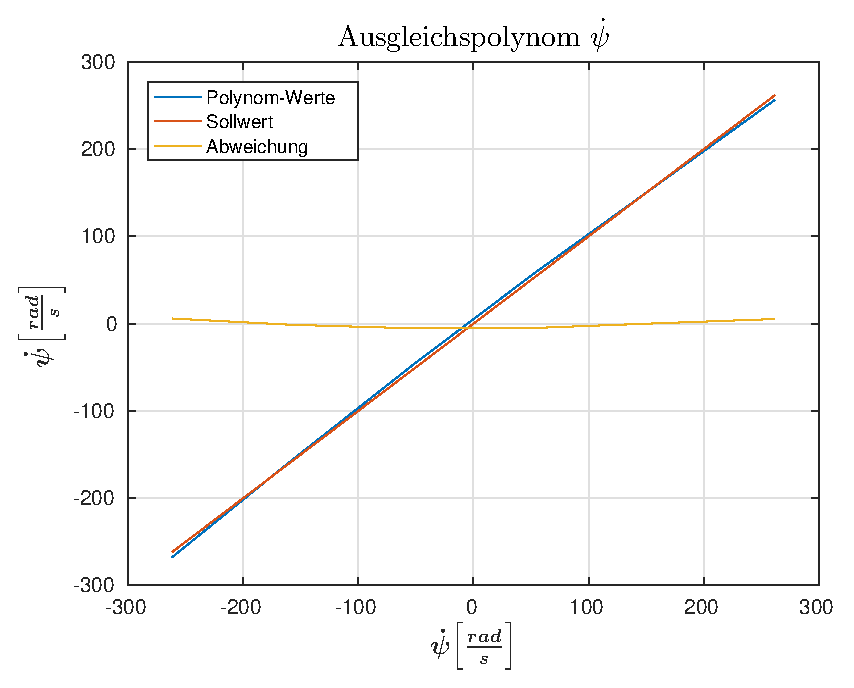
\includegraphics[width=0.5\linewidth]{img/ADC_mittelwert_polynom.eps}
\end{figure}

\subsection{Filterung der Zustandsgrößen}
In der Regel werden Sensoren von Störungen unterschiedlichster Art beeinflusst. Deshalb werden in diesem Abschnitt verschiedene Ansätze vorgestellt um die Zustandsgrößen $\varphi$, $\dot{\varphi}$ und $\dot{\psi}$ zu filtern. 

\subsubsection{Ansätze zur Filterung von $\varphi$}
Der Ausfallwinkel $\varphi$ kann wie bereits vorgestellt aus den Beschleunigungswerten geschätzt werden. Alternativ kann die aktuelle Winkelgeschwindigkeit $\dot{\varphi}$, welche mit Hilfe der Gyroscope gemessen wird, integriert werden. Beide Ansätze werden von unterschiedlichen Rauschsignale beeinflusst. Die Beschleunigungssensoren reagieren empfindlich auf hochfrequente Signale und verstärken diese. Dadurch sind die Winkelschätzungen, welche auf diesen Messwerten beruhen, von hochfrequenten Rauschsignalen betroffen. 
Die Gyroscope-Werte sind trotz der Justierung mit einem Offset behaftet. Durch die Integration dieses konstanten Signales ensteht ein tieffrequentes Rauschsignale, welches oftmals als Drift bezeichnet wird. 
Deshalb werden im Anschluss das Komplementär- und Kalman-Filter vorgestellt, wobei es sich um Methoden der Datenfusion handelt.

\subsubsubsection{Komplementär-Filter für $\varphi$}
Wie bereits erläutert liefert die Winkelschätzung aus den Beschleunigungswerten das verrauschte Signal $\varphi^A$ und die Integration der Gyroscopewerte $\varphi^G$.
\begin{equation}
\begin{split}
\varphi^A(s) &= \varphi(s) + x^A(s) \\
\varphi^G(s) &= \frac{1}{s} \cdot (\dot{\varphi}(s) + \dot{x}^G(s)) 
\end{split}
\end{equation}

Angenommen, dass $\varphi^A$ mit Hilfe eines Tiefpass und $\varphi^G$ mit Hilfe eines Hochpass gefiltert werden, so ergibt sich das folgende Blockschaltbild.

\begin{figure}[!h]
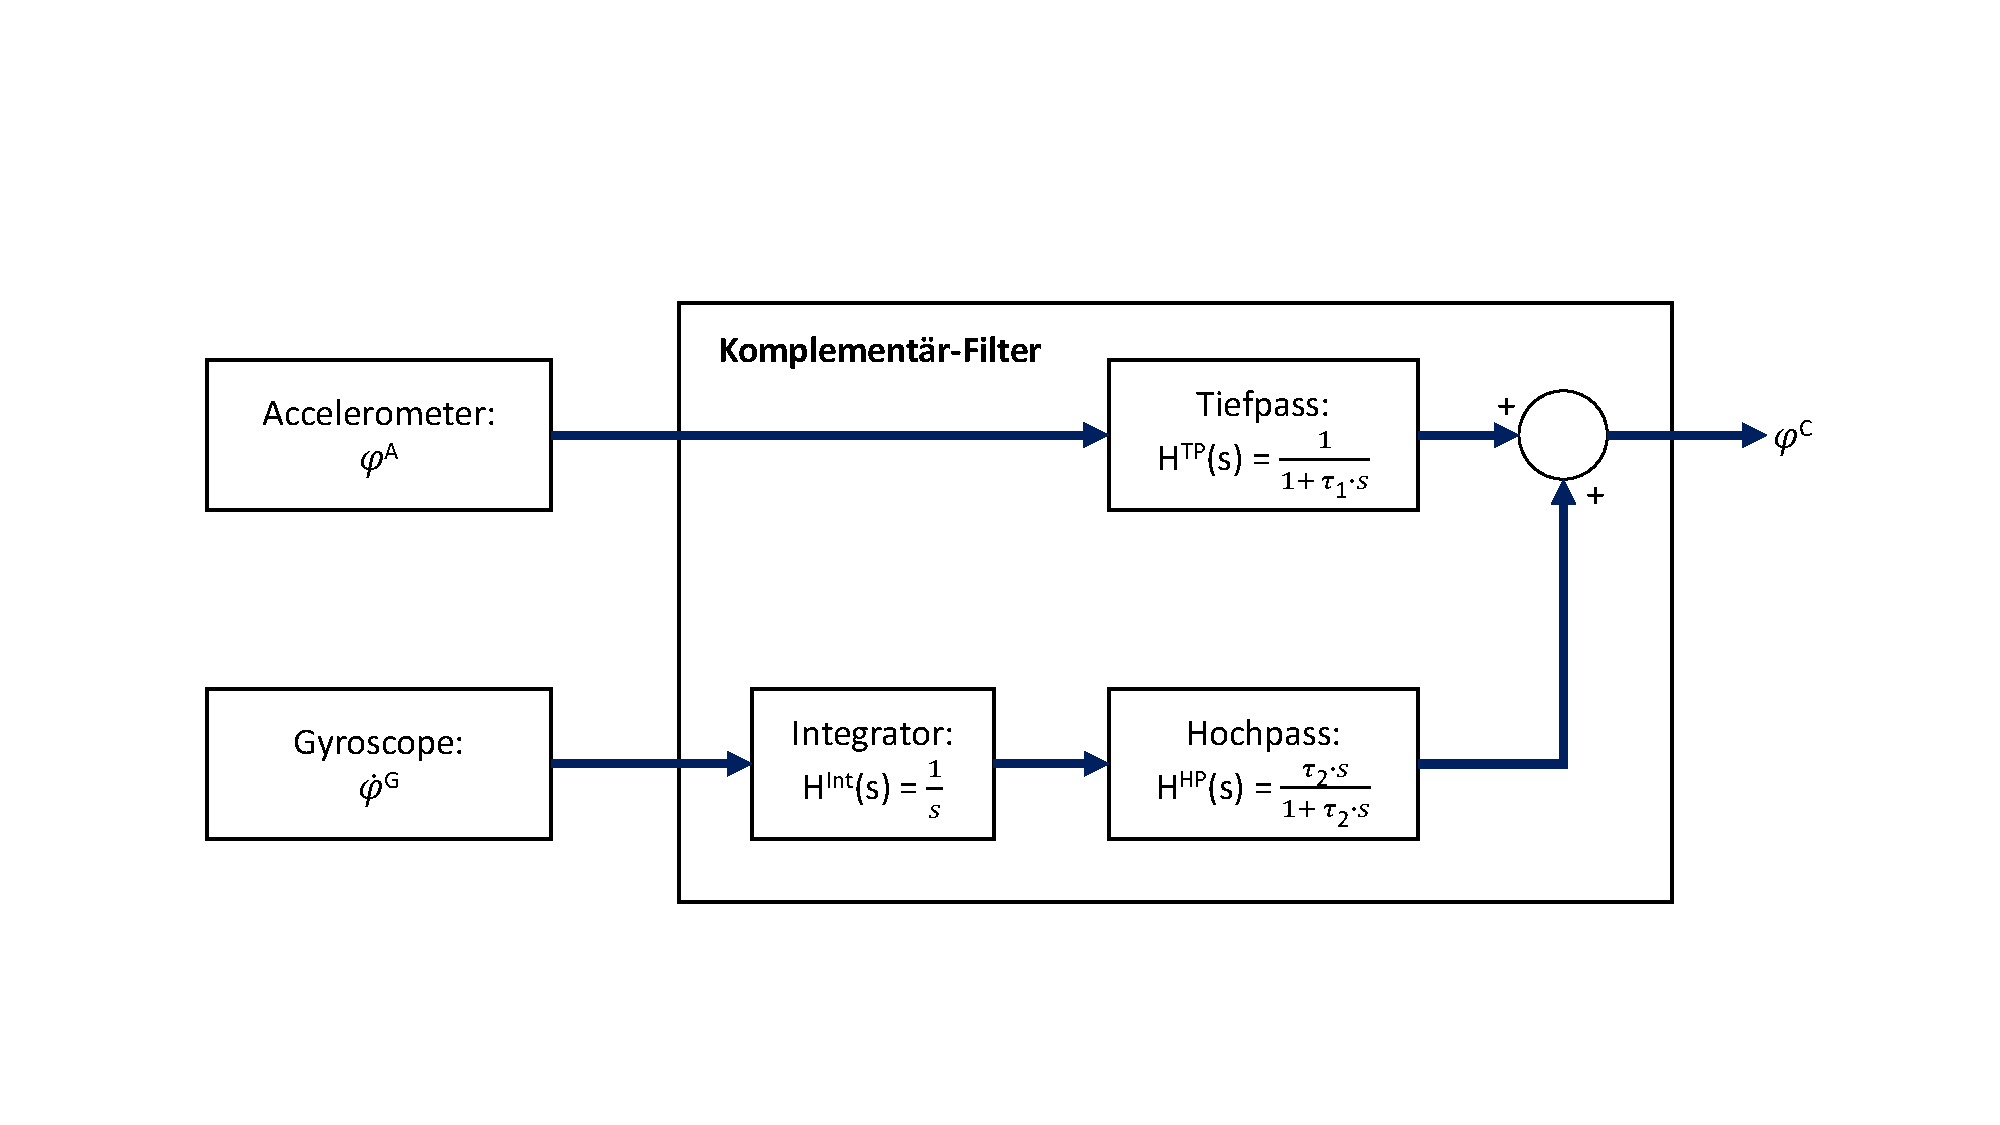
\includegraphics[scale=0.5,trim={0 3cm 0 4cm},clip]{img/Komp_CuBa_1D}
\end{figure}

Nach dem Blockschaltbild ergibt sich im Bildbereich der folgende Zusammenhang.

\begin{equation}
\label{comp_bildbereich_eq}
\begin{split}
\varphi^C(s) &= \frac{1}{1 + \tau_1 \cdot s} \cdot \varphi^A(s) + \frac{\tau_2 \cdot s}{1 + \tau_2 \cdot s} \cdot \frac{1}{s} \cdot \dot{\varphi}^G(s) \\
&= \frac{1}{1 + \tau_1 \cdot s} \cdot [\varphi(s) + x^A(s)] + \frac{\tau_2 \cdot s}{1 + \tau_2 \cdot s} \cdot [\varphi(s) + x^G(s)]
\end{split}
\end{equation}

Als erste Entwurfsbedinung müssen die beiden Zeikonstanten $\tau_1$ und $\tau_2$ so gewählt werden, dass die Rauschanteile $x^A$ und $x^G$ verschwinden. Falls dies gegeben ist, lässt sich (\ref{comp_bildbereich_eq}) vereinfachen.
\begin{equation}
\begin{split}
\varphi^C(s) &= \frac{1}{1 + \tau_1 \cdot s} \cdot \varphi(s) + \frac{\tau_2 \cdot s}{1 + \tau_2 \cdot s} \cdot \varphi(s) \\
&= \varphi(s) \cdot (\frac{1}{1 + \tau_1 \cdot s} + \frac{\tau_2 \cdot s}{1 + \tau_2 \cdot s})
\end{split}
\end{equation}
Falls die beiden Zeitkonsanten, unter Einhaltung der ersten Bedingung, gleichgesetzt werden können, ergibt sich die folgende Übertragungsfunktion für das Komplementär-Filter.
\begin{equation}
\tau = \tau_1 = \tau_2
\end{equation}
\begin{equation}
\varphi^C(s) = \varphi(s) \cdot (\frac{1}{1 + \tau \cdot s} + \frac{\tau \cdot s}{1 + \tau \cdot s}) = \varphi(s)
\end{equation}

Um die gennanten Bedinungen zu erfüllen muss eine Spektralanalyse der Rauschsignale durchgeführt werden. Welche verwendet wird um die Grenzfrequenzen des Hoch- und Tiefpassfilters festzulegen. Anschließend wird geprüft ob diese gleichgesetzt werden können.

Die Berechnung des Komplementär-Filters findet auf einem Digitalrechner statt. Somit muss (\ref{comp_bildbereich_eq}) in eine diskrete Berechnungsvorschrift transformiert werden. Hierfür können das Hochpassfilter und der Integrator zu einem Tiefpass zusammengeführt werden.
\begin{equation}
\label{Comp_Bild_eq}
\varphi^C(s) = \frac{1}{1 + \tau \cdot s} \cdot \varphi^A(s) + \frac{\tau}{1 + \tau \cdot s} \cdot \dot{\varphi}^G(s)
\end{equation}

Mit Hilfe der Backward-Euler-Tranformation kann (\ref{Comp_Bild_eq}) als Z-Transformierte dargestellt werden.
\begin{equation}
s = \frac{1 - z^{-1}}{T}
\end{equation}
\begin{equation}
\begin{split}
\varphi^C(z) & = \frac{1}{1 + \tau \cdot \frac{1 - z^{-1}}{T} } \cdot \varphi^A(z) + \frac{\tau}{1 + \tau \cdot \frac{1 - z^{-1}}{T}} = \\
& = \frac{T}{T + \tau - \tau \cdot z^{-1}} \cdot \varphi^A(z) + \frac{\tau \cdot T}{T + \tau - \tau \cdot z^{-1}} \cdot \dot{\varphi}^G(z)
\end{split}
\end{equation}

\begin{equation}
\begin{split}
(T + \tau - \tau \cdot z^{-1}) \cdot \varphi^C(z) = T \cdot \varphi^A(z) + \tau \cdot T \cdot \dot{\varphi}^G(z)
\end{split}
\end{equation}

\begin{equation}
(T + \tau) \cdot \varphi^C(z) = \tau \cdot [\varphi^C(z) \cdot z^{-1}  + T \cdot \dot{\varphi}^G(z)] + T \cdot \varphi^A(z)
\end{equation}

\begin{equation}
\begin{split}
\varphi^C(z) & = \frac{\tau}{\tau + T}[\varphi^C(z) \cdot z^{-1}  + T \cdot \dot{\varphi}^G(z)] + \frac{T}{T + \tau} \varphi^A(z) \\
& = \frac{\tau}{\tau + T}[\varphi^C(z) \cdot z^{-1}  + T \cdot \dot{\varphi}^G(z)] + (1 - \frac{\tau}{T + \tau}) \varphi^A(z)
\end{split}
\end{equation}

Durch die Substitution $\alpha = \frac{\tau}{\tau + T}$ kann weiter vereinfacht werden. 

\begin{equation}
\varphi^C(z)  = \alpha[\varphi^C(z) \cdot z^{-1}  + T \cdot \dot{\varphi}^G(z)] + (1 - \alpha) \varphi^A(z)
\end{equation}
\begin{equation}
\varphi^C_n = \alpha(\varphi^C_{n-1}  + T \cdot \dot{\varphi}^G_n) + (1 - \alpha) \varphi^A_n
\end{equation}

\subsubsubsection{Kalman-Filter für $\varphi$}
Das Kalman-Filter beruht auf dem Prinzip der Zustandsschätzung. Diese Schätzung erfolgt mittels der Messwerte aus Gyroskopen, Beschleunigungssensoren und der darauf folgenden Winkelschätzung. Hierbei greift der Algorithmus auf Methoden der Wahrscheinlichkeitsrechnung zurück. Ist die Varianz eines Messfehlers gegeben, so kann eine Schätzung des tatsächlichen Zustandes vorgenommen werden.
In diesem Fall wird mit den linearisierten Bewegungsgleichungen gearbeitet. Dadurch kann das gewöhnliche Kalman-Filter verwendet werden. Für nichtlineare Systeme müssen unterschiedliche Filteralgorithmen, wie beispielsweise das Extended-Kalman-Filter, verwendet werden.


\begin{table}[h!]
\centering
\begin{tabularx}{0.9\textwidth}{|c|c|}
\hline
 \textbf{Bezeichnung}  	& \textbf{Erkärung} \\ \hline
 $\boldsymbol{x}^*_n$	&	Systemzustände \\ \hline
 $\hat{\boldsymbol{x}}_n$ & Geschätzte Systemzustände \\ \hline 
 $\boldsymbol{u}_n$		& 	Messbare Eingangsgrößen  \\ \hline
 $\boldsymbol{v}_n$		&	Störgrößen \\ \hline
 $\boldsymbol{A}_d$ 	& 	Systemmatrix, welche den Systemzustand $\hat{\boldsymbol{x}}_n$  \\  & auf den folgenden Zeitschritt abbildet. \\ \hline
 $\boldsymbol{B}_d$		&	Eingangsmatrix \\ \hline
 $\boldsymbol{C}_d$		&	Ausgangsmatrix \\ \hline
 $\boldsymbol{P}^*_n$	&	Kovarianzmatrix von $\boldsymbol{x}^*_n$. Legt die Sicherheit der Schätzung fest. \\ \hline
 $\hat{\boldsymbol{P}}_n$ & Filterkovarianzmatrix von $\hat{\boldsymbol{x}}_n$. Gibt die Gewichtung der Messwerte an. \\ \hline
 $\boldsymbol{Q}_n$		&	Kovarianzmatrix des Systemrauschens \\ \hline
 $\boldsymbol{R}_n$		& 	Kovarianzmatrix des Messrauschens \\ \hline
\end{tabularx}
\end{table}

Die Berechnung des Kalman-Filters verläuft in zwei Schritten, welche in insgesamt fünf Teile gegliedert ist. Zuerst wird der Prädikationsschritt durchgeführt, hierbei wird der Prädikationsschätzwert $\boldsymbol{x}^*_{n+1}$ berechnet, welcher den Systemzustand im folgenden Zeitschritt darstellt. Zusätzlich wird die Prädikationskovarianzmatrix $\boldsymbol{P}^*_{n+1}$ berechnet, welche angibt wie sicher die Vorhersage im Verhältnis zu dem wahren Systemzustand ist.
Im zweiten Abschnitt, der s.g. Korrektur- bzw. Filterschritt, wird die Vorhersage mit Hilfe der neuen Messwerte korrigiert. Hierfür wird zuerst die Verstärkungsmatrix $\boldsymbol{K_{n+1}}$ berechnet, welche den Rückkopplungsfaktor der Messwerte wiedergibt. Im Anschluss wird der Endschätzwertes des Systemzustandes mit Hilfe des ersten Prädikationswertes $\boldsymbol{x}^*_{n+1}$ und der Verstärkungsmatrix $\boldsymbol{K}_{n+1}$ bestimmt. Zuletzt wird die Varianz des geschätzten Systemzustandes $\hat{\boldsymbol{P}}_{n+1}$ berechnet.

\begin{enumerate}
	\item \textbf{Prädikationsschätzwert}
	\newline
	Der Systemzustand zum Zeitpunkt $n$ ist beschreibbar durch die zeitdiskrete, lineare, stochastische Differenzengleichung
	\begin{equation}
	\boldsymbol{x}^*_{n+1} = \boldsymbol{A}_d \cdot \boldsymbol{\hat{x}}_n + \boldsymbol{B} \cdot \boldsymbol{u}_n + \boldsymbol{v}_n
	\end{equation}
	Die Systemmatrix $\boldsymbol{A}$ bildet den Systemzustand $\boldsymbol{\hat{x}}$ von Zeitschritt $n$ auf den folgenden Zeitschritt $n+1$ ab. Die Eingangsgrößen $\boldsymbol{u}_n$ werden durch die Matrix $\boldsymbol{B}$ auf den Systemzustand $\boldsymbol{x}^*_{n+1}$ abgebildet. Das Rasuchen bzw. die äußeren Störeinflüsse werden durch den additiven Term $\boldsymbol{v}_n$ repräsentiert.
	\item \textbf{Prädikationskovarianzmatrix}
	\newline
	Die Kovarianzmatrix $\boldsymbol{P}^*_{n+1}$ gibt an, wie sicher die Prädikation im Verhältnis zu dem wahren Systemzustand ist.
	\begin{equation}
	\boldsymbol{P}^*_{n+1} = \boldsymbol{A} \cdot \boldsymbol{\hat{P}}_n \cdot \boldsymbol{A}^T + \boldsymbol{Q}_n
	\end{equation}
	\item \textbf{Verstärkungsmatrix} \newline
	Die Verstärkungsmatrix $\boldsymbol{K}_{n+1}$ wird für die Korrektur der Vorhersage verwendet. Sie bestimmt, mit welcher Verstärkung der Messvektor rückgekoppelt wird.
	\begin{equation}
	\boldsymbol{K}_{n+1} = (\boldsymbol{P}^*_{n+1} \cdot \boldsymbol{C}^T)(\boldsymbol{C} \cdot \boldsymbol{P}^*_{n+1} \cdot \boldsymbol{C}^T + \boldsymbol{R}_{n+1})^{-1}
	\end{equation}
	\item \textbf{Filterschätzwert}
	Mit Hilfe der Verstärkungsmatrix $\boldsymbol{K}_{n+1}$ und des Prädikationswertes $\boldsymbol{x}^*_{n+1}$ wird der finale Schätzwert des Systemzustandes zu dem Zeitpunkt $n+1$ bestimmt.
	\begin{equation}
	\boldsymbol{\hat{x}}_{n+1} = \boldsymbol{x}^*_{n+1} + \boldsymbol{K}_{n+1}(\boldsymbol{y}_{n+1} - \boldsymbol{C} \cdot \boldsymbol{x}^*_{n+1})
	\end{equation}
	\item \textbf{Filterkovarianzmatrix}
	Im letzten Schritt wird die Varianz des geschätzten Systemzustandes berechnet, welche die Gewichtung der Messwerte im weiteren Verlauf der Berechnung beschreibt.
	\begin{equation}
	\boldsymbol{\hat{P}}_{n+1} = \boldsymbol{P}^*_{n+1} - \boldsymbol{K}_{n+1} \cdot \boldsymbol{C} \cdot \boldsymbol{P}^*_{n+1}
	\end{equation}
\end{enumerate}

\subsubsubsection*{Anwendung des Kalman-Filters}
Um die zuvor angesprochenen Nachteile der einzelnen Sensoren auszugleichen, wird nun die Umsetzung eines Kalman-Filters zur Sensorfusion vorgestellt.

Das Kalman-Filter fusioniert den Ausfallwinkel $\varphi_{Acc}$ aus der Winkelschätzung mit der Winkeländerung $\Delta \varphi_{Gyr}$, welche durch Integration der Gyroskopwerte gewonnen wurde. Daraus ergibt sich der gefilterte Winkel $\hat{\varphi}_n$. Dieser gefilterte Zustandswert wird für die Berechnung des Regelkreises verwendet.

Als absolute Eingangsgrößen stehen hier zum einen die Winkelschätzung $\varphi_{Acc}$ und die Winkeländerung $\Delta \varphi_{Gyr}$ zur Verfügung. Somit kann das fehlerbehaftete Teilsystem durch folgende Gleichungen beschrieben werden, wobei $v_{Gyr,n}$ $w_{Acc,n}$ die störbehafteten Additionstherme darstellen.

\begin{equation}
\varphi_{n+1} = \varphi_{n} + \Delta \varphi_{Gyr,n} + v_{Gyr,n}
\end{equation}
\begin{equation}
\varphi_{Acc,n} = \varphi_n + w_{Acc,n}
\end{equation}

\begin{figure}[!h]
\centering
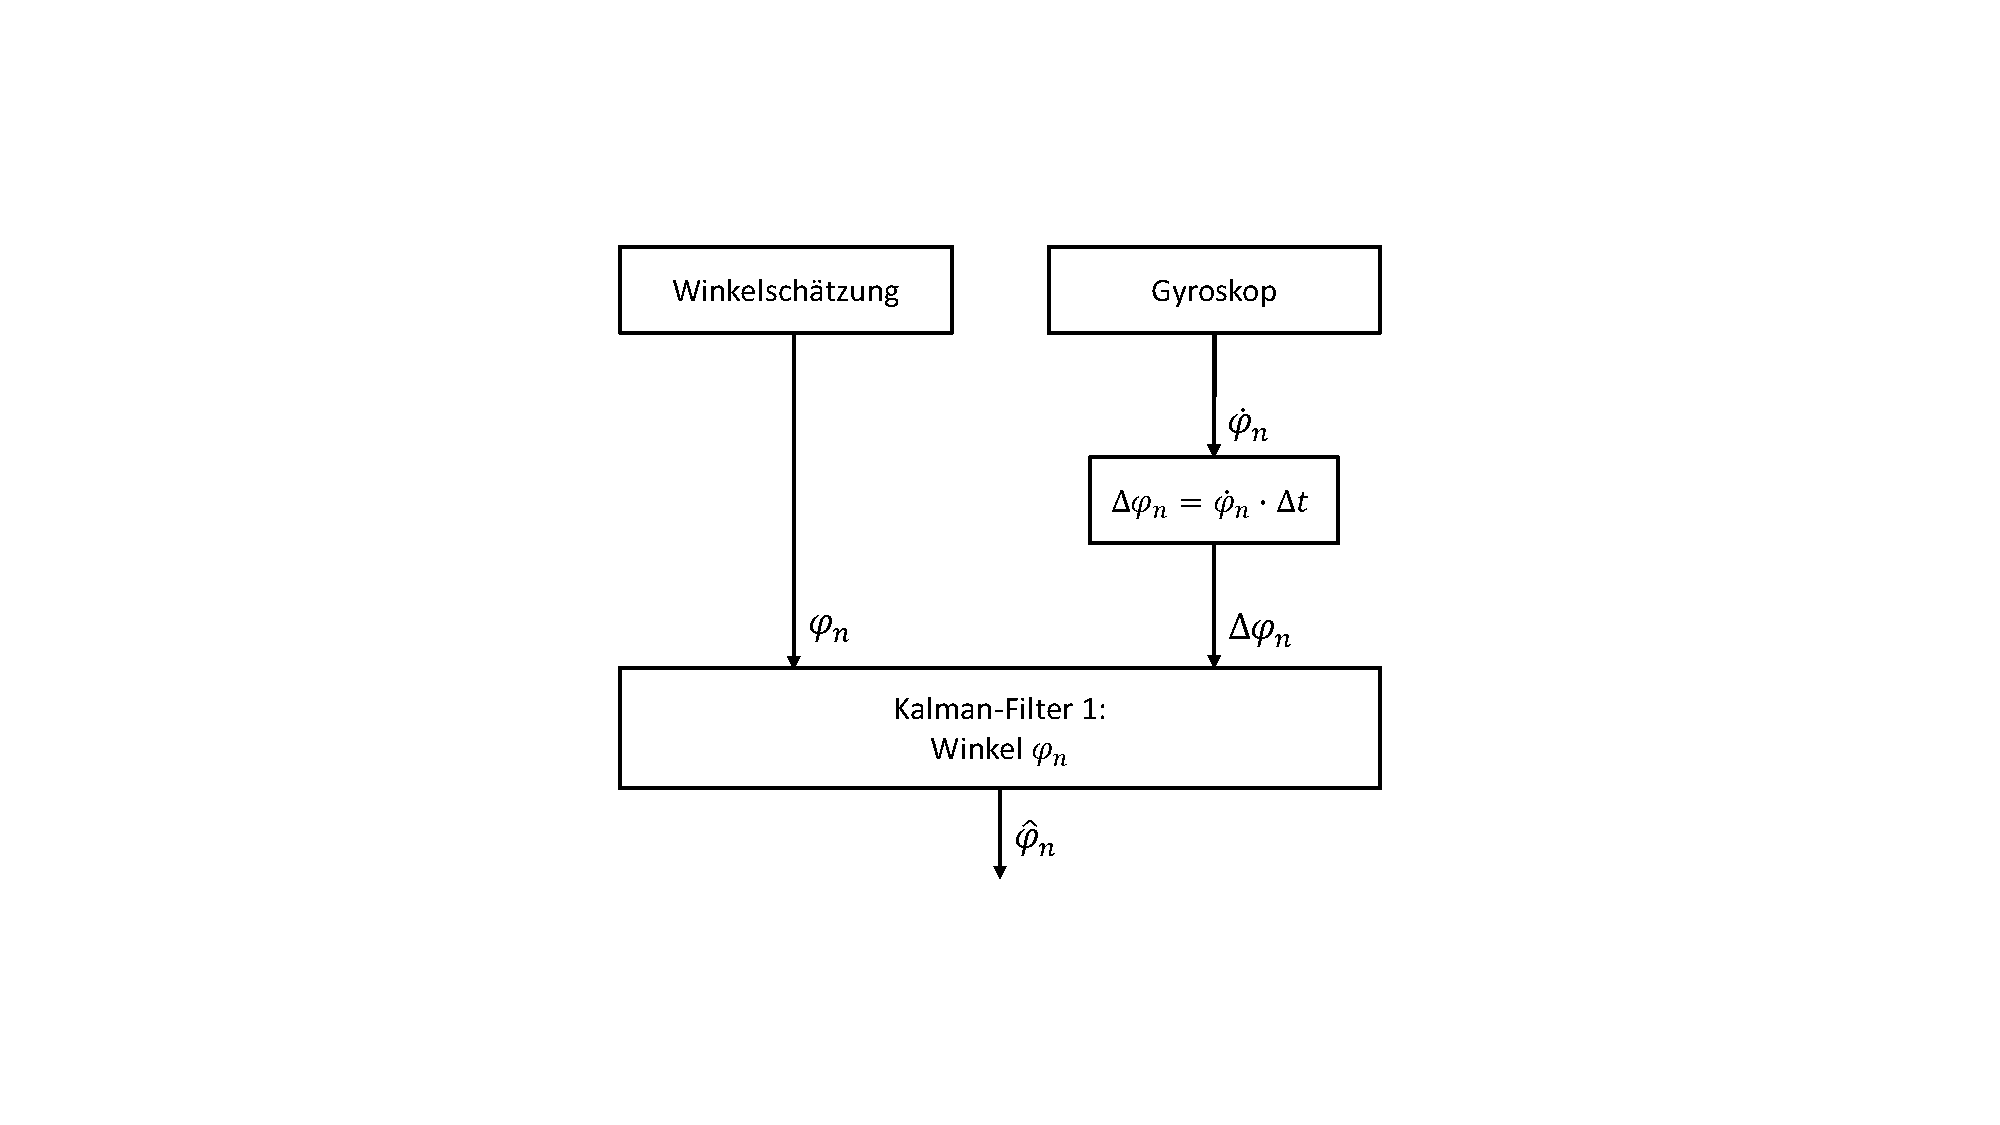
\includegraphics[width=0.8\linewidth, trim={0 3.5cm 0 3.5cm},clip]{img/kalman_phi_overview}
\caption{Übersicht Kalman-Filter, Quelle: eigene Darstellung}
\end{figure}

Die bereits vorgestellten Berechnungsschritte können nun auf den spezifischen Anwendungsfall angepasst werden. Da lediglich eine einzelne Zustandsgröße berechnet wird, werden anstelle von Vektoren und Matrizen skalare Größen verwendet.

\begin{enumerate}
\item \textbf{Prädikationsschätzwert}
\begin{equation}
\varphi^*_{n+1} = \hat{\varphi}_n + \Delta \varphi_{Gyr,n}
\end{equation}
\item \textbf{Prädikationsvarianz}
\begin{equation}
P^*_{n+1} = \hat{P}_{n+1} + \sigma^2(\Delta \varphi_{Gyr,n})
\end{equation}
\item \textbf{Verstärkungsfaktor}
\begin{equation}
K_{n+1} = \frac{P^*_{n+1}}{P*_{n+1} + \sigma^2(\varphi_{Acc,n}}
\end{equation}
\item \textbf{Filterschätzwert}
\begin{equation}
\hat{\varphi}_{n+1} = \varphi^*_{n+1} + K_{n+1} \cdot (\varphi_{Acc,n} - \varphi^*_{n+1})
\end{equation}
\item \textbf{Filtervarianz}
\begin{equation}
\hat{P}_{n+1} = (1-K_{n+1}) \cdot P^*_{n+1}
\end{equation}
\end{enumerate}

\subsubsubsection{Vergleich der Filter}
Um einen ersten Eindruck über die Qualität der Filter zu erhalten wird die Würfelseite als gewöhnliches Pendel aufgebaut und in Schwingung versetzt. Anschließend werden die Sensorwerte ausgewertet und die beiden Filter berechnet. 

\begin{figure}[h!]
\centering
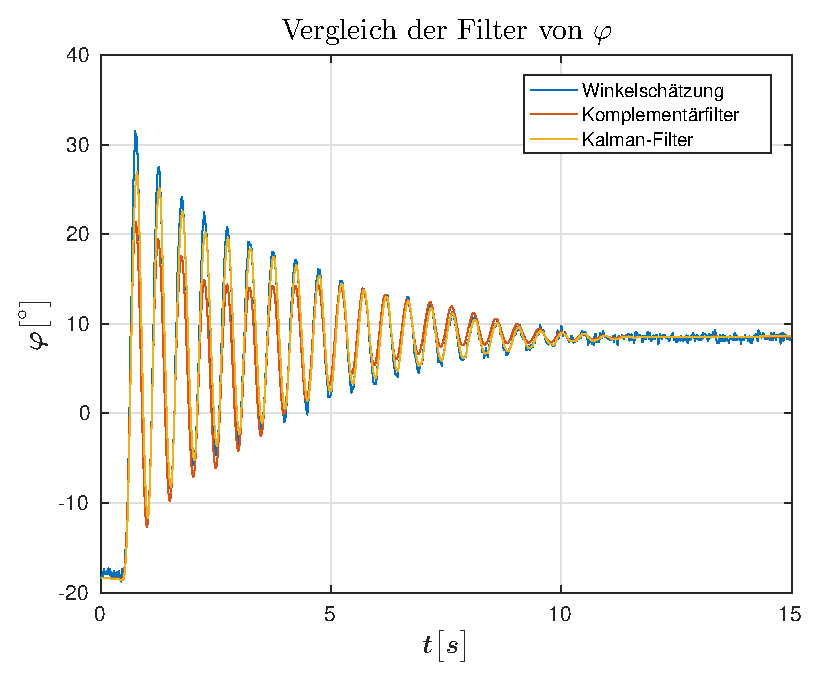
\includegraphics[width=0.5\linewidth]{img/filtervergleich_phi}
\caption{Vergleich der Filter für $\varphi$, Quelle: eigene Darstellung}
\end{figure}

Aus dem Verlauf der Signale lässt sich erkennen, dass die beiden Filter zu einer Glättung führen. Dennoch unterscheiden sich die Amplituden der drei Signale stark voneinander. Allerdings lassen sich diese Verläufe ohne ein Referenzsignal nicht weiter beurteilen. Somit kann eine endgültige Bewertung der Filter erst an Hand der Güte des geschlossenen Regelkreises getroffen werden.

\subsubsection{Ansätze zur Filterung von $\dot{\varphi}$}
Um die Winkelgeschwindigkeit $\dot{\varphi}$ zu ermitteln wird ebenfalls ein Kalman-Filter eingesetzt.
 
\begin{figure}[H]
\centering
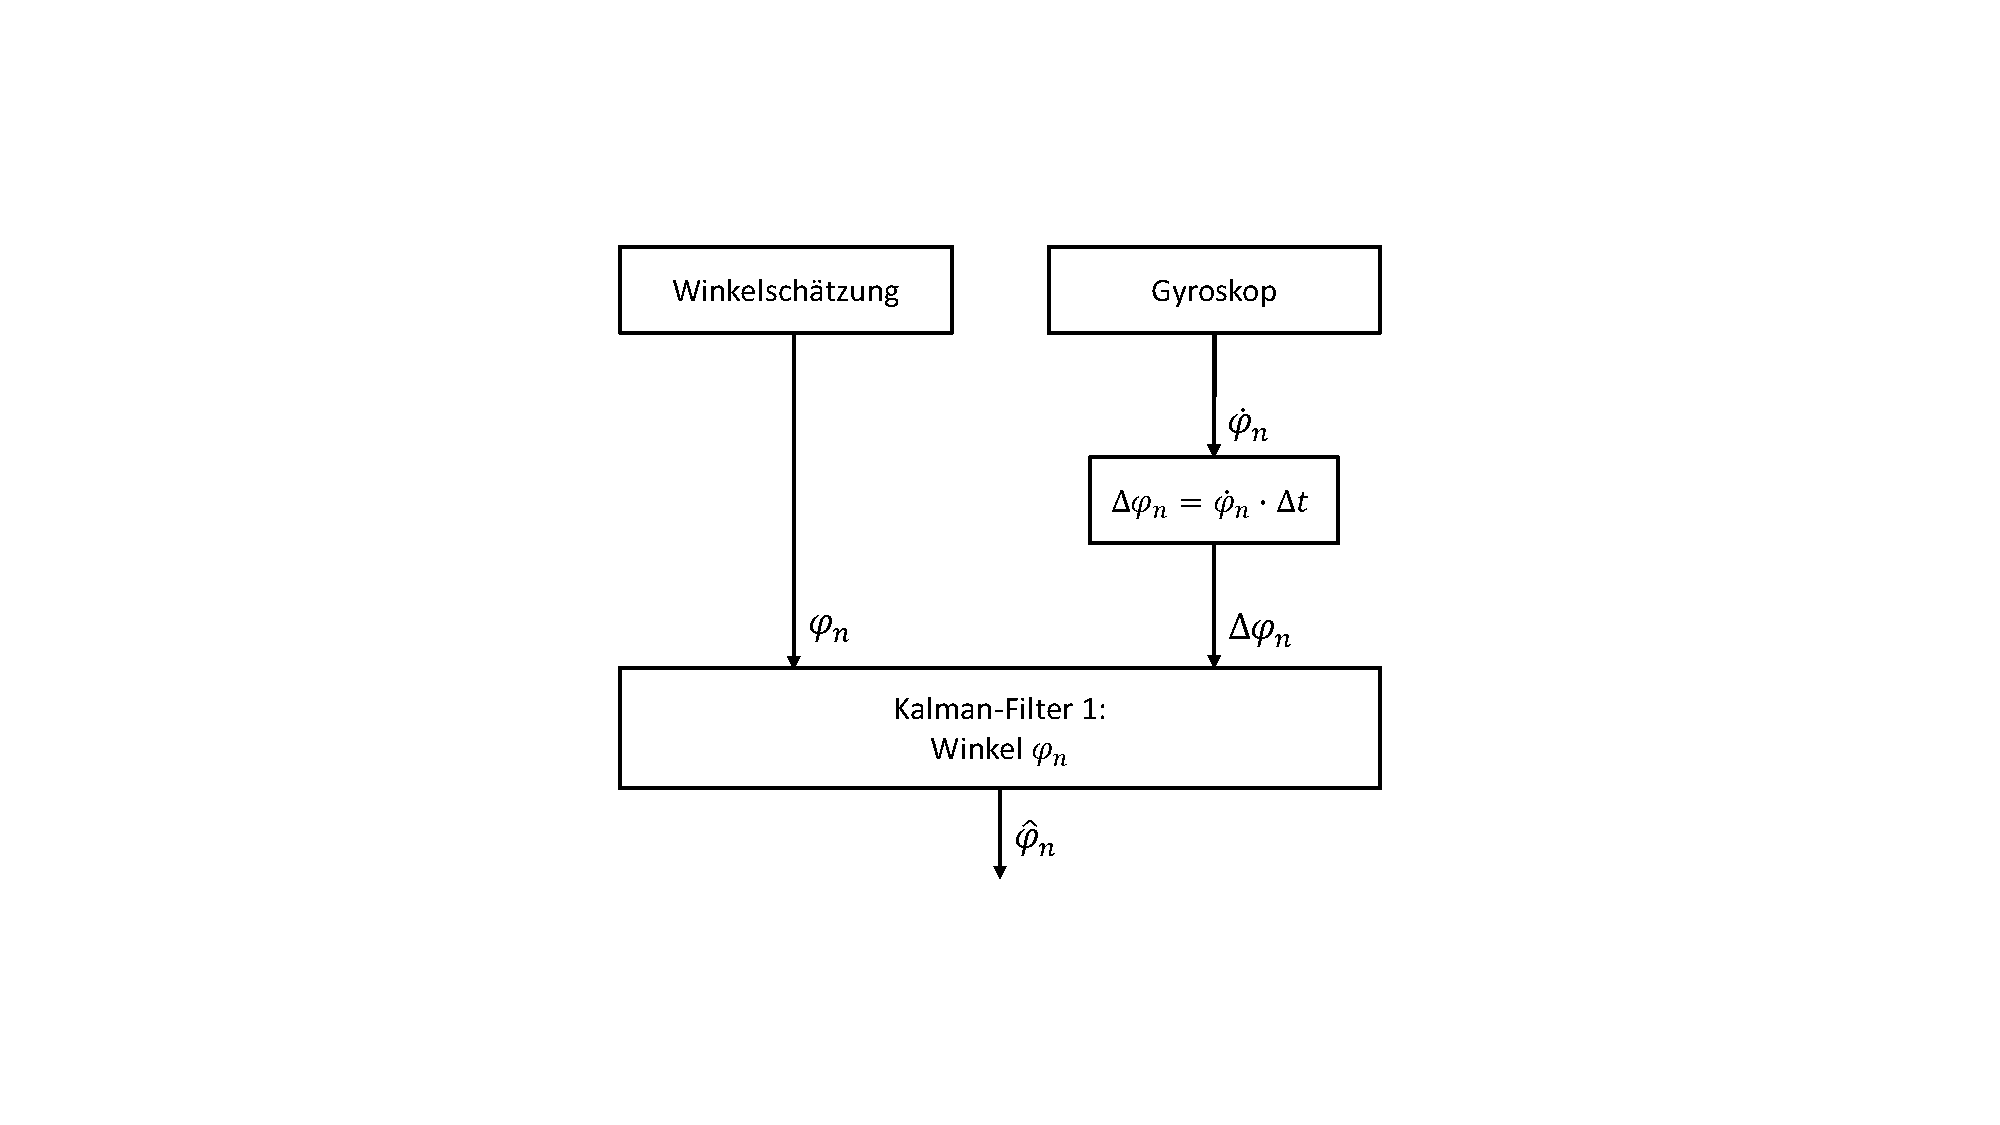
\includegraphics[width=0.8\linewidth, trim={0 3.7cm 0 3.7cm},clip]{kalman_phi__d_overview}
\vspace*{-\baselineskip}
\end{figure}

In diesem Fall werden als Eingangsignale der Messwert des Gyroscopes $\dot{\varphi}_{Gyr}$ und integrierte Winkelbeschleunigung $\dot{\varphi}_{Acc}$ verwendet. Somit kann das fehlerbehaftete Teilsystem in seiner Dynamik durch folgende Gleichungen beschrieben werden, wobei die Störanteile der Beschleunigungssensoren und Gyroscope durch $v_{Acc,n}$ bzw. $w_{Gyr,n}$ dargestellt werden.
\begin{equation}
\dot{\varphi}_{n+1} = \dot{\varphi}_n + \Delta \dot{\varphi}_{Acc,n} + v_{Acc,n}
\end{equation}
\begin{equation}
\dot{\varphi}_{Gyr,n} = \dot{\varphi}_n + w_{Gyr,n}
\end{equation}
Die Zustandsschätzung verläuft analog zu dem bereits vorgestellten Verfahren.
\begin{enumerate}
\item \textbf{Prädikationsschätzwert}
\begin{equation}
\dot{\varphi}^*_{n+1} = \hat{\dot{\varphi}}_n + \Delta \dot{\varphi}_{Acc,n}
\end{equation}
\item \textbf{Prädikationsvarianz}
\begin{equation}
P^*_{n+1} = \hat{P}_{n+1} + \sigma^2(\Delta \dot{\varphi}_{Acc,n})
\end{equation}
\item \textbf{Verstärkungsfaktor}
\begin{equation}
K_{n+1} = \frac{P^*_{n+1}}{P*_{n+1} + \sigma^2(\dot{\varphi}_{Gyrs,n}}
\end{equation}
\item \textbf{Filterschätzwert}
\begin{equation}
\hat{\dot{\varphi}}_{n+1} = \dot{\varphi}^*_{n+1} + K_{n+1} \cdot (\dot{\varphi}_{Gyr,n} - \dot{\varphi}^*_{n+1})
\end{equation}
\item \textbf{Filtervarianz}
\begin{equation}
\hat{P}_{n+1} = (1-K_{n+1}) \cdot P^*_{n+1}
\end{equation}
\end{enumerate}
Die nächste Abbildung zeigt den Verlauf der Gyroscopewerte und des Kalman-Filters bei dem Versuch aus dem vorherigen Abschnitt.
\begin{figure}[!h]
\centering
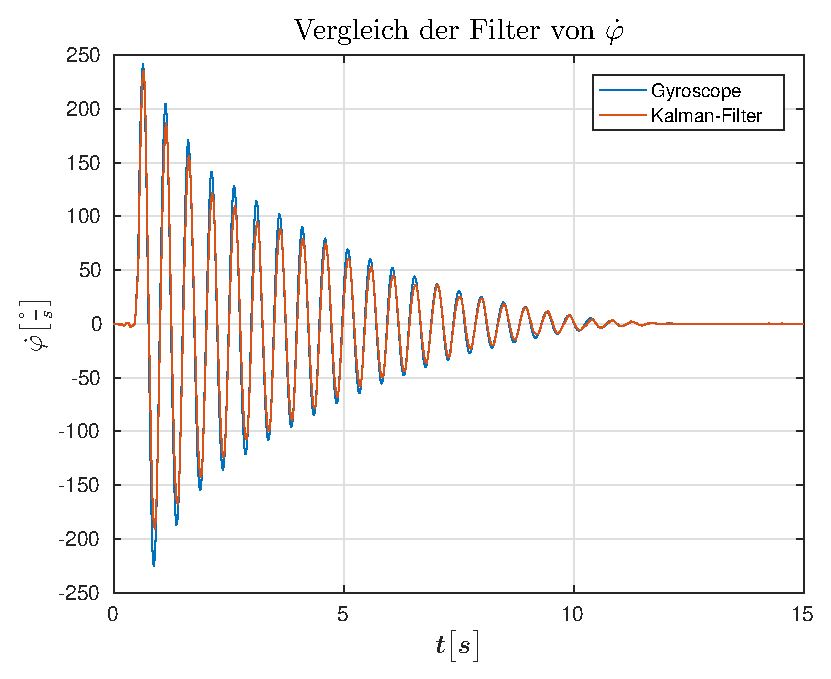
\includegraphics[width=0.5\linewidth]{img/filtervergleich_phi__d}
\caption{Verlauf des Filters für $\dot{\varphi}$, Quelle: eigene Darstellung}
\end{figure}
Hier sind nur marginale Unterschiede zwischen den Amplituden zu erkennen. Ebenso wie die Filter für $\varphi$ muss die letzendliche Filtergüte am geschlossenen Regelkreis näher untersucht werden.

\newpage
\subsubsection{Ansätze zur Filterung von $\dot{\psi}$}
Die Winkelgeschwindigkeit $\dot{\psi}$ des Motors wird als analoges Signal von einem 12-Bit AD-Wandler ausgewertet. Diese Messwerte sind ebenfalls von hochfrequenten Störeinflüssen betroffen und müssen somit geglättet werden. Hierfür werden digitale Tiefpassfilter verwendet, welche in Form eines gleitenden Mittelwertes implementiert. Dieser Mittelwert wird über die letzten $N$ Messwerte gebildet. 

\begin{equation}
y_n = \frac{1}{N}\sum^{N-1}_{k=0} x_{n-k}
\end{equation}

Die Glättung des Filters nimmt mit der Anzahl der verwendeten Werte $N$ zu, allerdings wird das Filter damit auch träger. Somit muss ein Kompromiss zwischen Verzögerung und Glättung gefunden werden. Die folgende Abbildung zeigt den Vergleich der nicht gefilterten Werte aus dem Versuch zur Bestimmung des Reibwertes $C_{\psi}$ und verschiedenen Mittelwert-Filtern. 

\begin{figure}[!h]
\centering
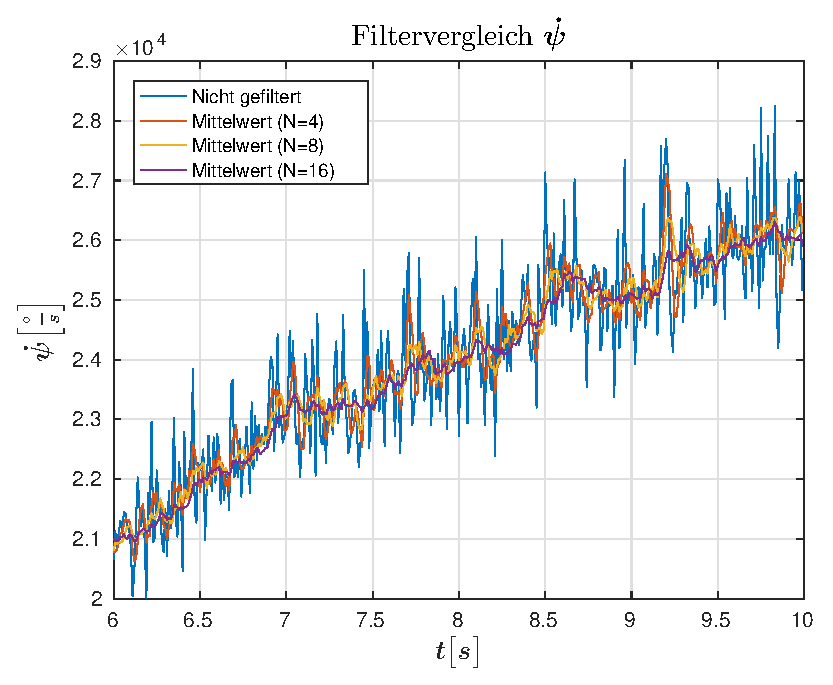
\includegraphics[width=0.6\linewidth]{img/filtervergleich_psi__d}
\end{figure}

Der Verlauf zeigt deutlich die Glättung des Signales. Außerdem ist keine signifikante Verzögerung durch die verschiedenen Filter ersichtlich. Allerdings ist zu erwarten, dass der Motor ein Eingangssignal mit höheren Frequenzanteilen erzeugt, sobald der Regelkreis geschlossen wird. Die hochfrequenten Signalanteile werden durch die Tiefpassfilter entfernt, wodurch ggf. eine Verfälschung des Eingangssignales entsteht. Deshalb kann die optimale Konfiguration des Mittelwert-Filters erst an der realen Regelstrecke ermittelt werden.
\subsection{Modellbildung und Bestimmung der Systemgrößen}
Mit Hilfe der Bewegungsgleichungen aus Abschnitt \ref{Dynamik_sec} kann nun eine Zustandsraumdarstellung aufgestellt werden. Hierfür werden die nichtlinearen Terme entsprechend linearisiert. Mit Hilfe der Bewegungsgleichungen bzw. Zustandsraumdarstellung kann ein Simulink-Modell implementiert werden um das Systemverhalten zu simulieren. Mit Hilfe der Zustandsraumdarstellung wird ein Zustandsregler entworfen, welcher an dem Modell erprobt werden kann. Zusätzlich über die Simulation der Einfluss der einzelnen Parameter, Sensorrauschen und Störungen untersucht werden.

\begin{equation}
\textbf{x} = \begin{pmatrix}
\varphi \\ \dot{\varphi} \\ \dot{\psi}
\end{pmatrix}
\hspace{35pt}
\textbf{y} = \begin{pmatrix}
\varphi \\ \dot{\varphi} \\ \dot{\psi}
\end{pmatrix}
\hspace{35pt}
u = T_M
\end{equation}

\begin{equation}
\dot{\textbf{x}} = \textbf{A} \cdot \textbf{x} + \textbf{B} \cdot u
\end{equation}
\begin{equation}
\textbf{y} = \textbf{C} \cdot \textbf{x} + \textbf{D} \cdot u
\end{equation}
\begin{equation}
\setlength{\jot}{10pt}
\begin{split}
\renewcommand*{\arraystretch}{1.7}
\textbf{A} = \begin{pmatrix}
0 & 1 & 0 \\
\frac{g(m_K \cdot l_{AC} + m_R \cdot l_{AB})}{{\theta}^A_K + m_R \cdot l_{AB}^2} &
\frac{-C_{\varphi}}{{\theta}^A_K + m_R \cdot l_{AB}^2} & 
\frac{C_{\psi}}{{\theta}^A_K + m_R \cdot l_{AB}^2} \\
\frac{-g(m_K \cdot l_{AC} + m_R \cdot l_{AB)}}{{\theta}^A_K + m_R \cdot l_{AB}^2} &
\frac{C_{\varphi}}{{\theta}^A_K + m_R \cdot l_{AB}^2} &
\frac{-C_{\psi}({\theta}^A_K + {\theta}^B_R + m_R \cdot l_{AB}^2)}{{\theta}^B_R({\theta}^A_K + m_R \cdot l_{AB}^2)}
\end{pmatrix} 
\\
\renewcommand*{\arraystretch}{1.7}
\textbf{B} = \begin{pmatrix}
0 \\ \frac{-1}{{\theta}^A_K + m_R \cdot l_{AB}^2} \\ \frac{{\theta}^A_K + {\theta}^B_R + m_R \cdot l_{AB}^2}{{\theta}^K_R({\theta}^A_K + m_R \cdot l_{AB}^2}
\end{pmatrix}
\hspace{35 pt}
\textbf{C} = \begin{pmatrix}
1 & 1 & 1
\end{pmatrix}
\hspace{35pt}
\textbf{D} = \begin{pmatrix}
0
\end{pmatrix}
\end{split}
\end{equation}

\subsubsection{Identifikation der Parameter}
Der Reglerentwurf und die Simulation erfordern eine möglichst präzise Bestimmung der Systemparameter, wie z.B. Längen, Massen, Massenträgheitsmomente und Reibwerte. Die Bestimmung der Längen $l_{AB}$ und $l_{AC}$, der Massen $m_K$, $m_R$ und $m_G$, der Massenträgheitsmomente $\theta^A_K$ und $\theta^B_R$ erfolgt über das CAD-Modell. Hierfür werden Bauteile mit einer nicht homogenen Massenverteilung, wie z.B. die Motoren, in separate Baugruppen mit homogener Massenverteilung unterteilt.

\subsubsubsection{Ermittlung des Reibwertes $C_{\varphi}$}
In dem die Schwungmasse fest mit der Würfelseite verbunden wird ergibt sich die folgende Bewegungsgleichung für das Gesamtsystem.

\begin{equation}
\label{ermittlung_c_phi_equation}
(\theta^A_K + \theta^B_R + m_R  \cdot l_{AB}^2) \ddot{\varphi} = g(m_K \cdot l_{AC} + m_R \cdot l_{AB})sin(\varphi) - C_{\varphi} \cdot \dot{\varphi}
\end{equation}

In dem Versuchsaufbau wird das Gesamtsystem nun von einem Startwinkel $\varphi_0$ losgelassen, woraufhin eine gedämpfte Schwingung entsteht. Mit Hilfe der Sensoren können die Größen $\varphi$, $\dot{\varphi}$ und $\ddot{\varphi}$ gemessen werden.

\begin{figure}[h!]
\centering
 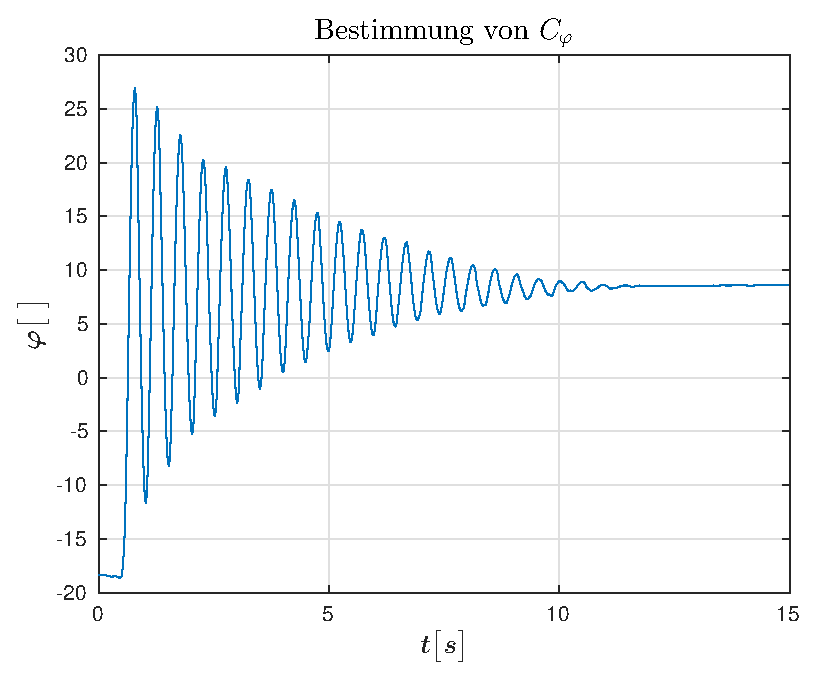
\includegraphics[width=0.5\linewidth]{img/C_phi.eps}
	\caption{Ausfallwinkel der Würfelseite bei Versuch 4, Quelle: eigene Darstellung}
\end{figure}

Über die $n$ Messpunkte ergeben sich die folgenden Vektoren.

\begin{equation}
\boldsymbol{\varphi} = \begin{pmatrix} \varphi_1 \\ \varphi_2 \\ \vdots \\ \varphi_n \end{pmatrix} \hspace{35pt}
\boldsymbol{\dot{\varphi}} = \begin{pmatrix}
\dot{\varphi_1} \\ \dot{\varphi_2} \\ \vdots \\ \dot{\varphi_n}
\end{pmatrix} \hspace{35pt}
\boldsymbol{\ddot{\varphi}} = \begin{pmatrix}
\ddot{\varphi_1} \\ \ddot{\varphi_2} \\ \vdots \\ \ddot{\varphi_n}
\end{pmatrix}
\end{equation}

Damit ergibt sich durch Umstellen von \ref{ermittlung_c_phi_equation} die folgende Gleichung.

\begin{equation}
C_{\varphi} \cdot \boldsymbol{\dot{\varphi}} = g(m_K \cdot l_{AC} + m_R \cdot l_{AB})sin(\boldsymbol{\varphi}) - (\theta^A_K + \theta^B_R + m_R  \cdot l_{AB}^2) \boldsymbol{\ddot{\varphi}}
\end{equation}

Mit Hilfe der Methode der kleinsten Fehlerquadrate kann nun der Reibwert $C_{\varphi}$ bestimmt werden.

\begin{equation}
C_{\varphi} = 5.4 \cdot 10^{-3} \cdot kg \cdot m^2 \cdot s^{-1}
\end{equation}


\subsubsubsection{Ermittlung des Reibwertes $C_{\psi}$}
Im nächsten Versuchsaufbau wird die Würfelseite fixiert ($\dot{\varphi} = 0$). Hierbei beschleunigt der Motor die Schwungmasse mit einem konstanten Drehmoment $T_M=10mNm$. $T_M$ ist so zu wählen, dass sich die Radgeschwindigkeit $\dot{\psi}$ in einem Bereich bewegt, welcher dem Arbeitsbereich des geschlossenen Regelkreises entspricht. 

\begin{figure}[h!]
\centering
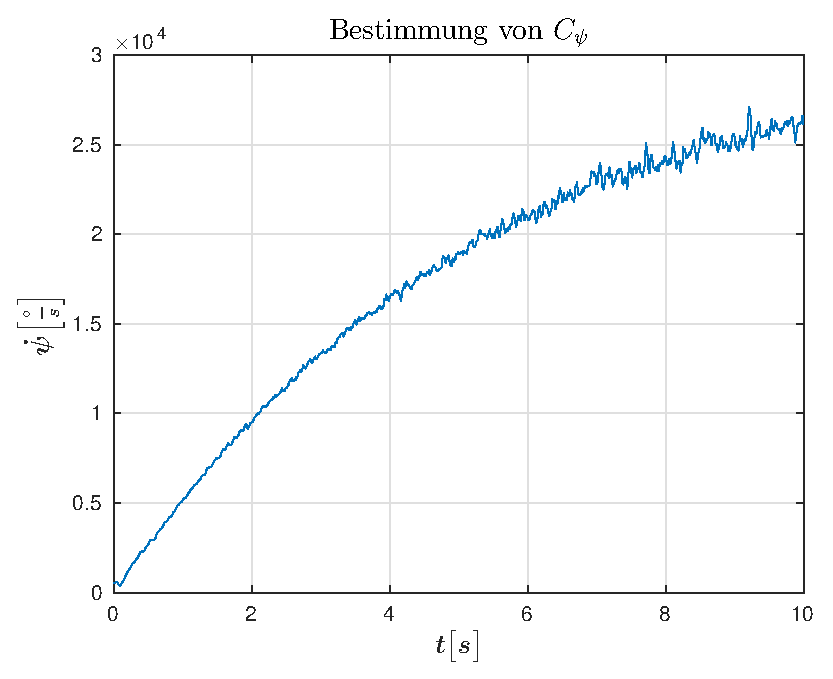
\includegraphics[width=0.6\linewidth]{img/C_psi.eps}
\caption{Versuch 5: Verlauf der Radgeschwindigkeit, Quelle: eigene Darstellung}
\end{figure}


Da die Bewegung auf einen Freiheitsgrad beschränkt wurde vereinfacht sich das Modell des Systems auf die folgende Bewegungsgleichung.

\begin{equation}
\label{ermittlung_c_psi_equation}
\theta^B_R \cdot \ddot{\psi} = T_M - C_\psi \cdot \dot{\psi}
\end{equation}

Im Versuchsverlauf werden bei $n$ Stützstellen die Werte von $\psi$, $\dot{\psi}$ und $\ddot{\psi}$ gemessen. Daraus ergeben sich die folgenden Vektoren.

\begin{equation}
\label{ermittlung_c_psi_vektoren_equation}
\boldsymbol{\psi} = \begin{pmatrix} \psi_1 \\ \psi_2 \\ \vdots \\ \psi_n \end{pmatrix} \hspace{35pt}
\boldsymbol{\dot{\psi}} = \begin{pmatrix}
\dot{\psi_1} \\ \dot{\psi_2} \\ \vdots \\ \dot{\psi_n}
\end{pmatrix} \hspace{35pt}
\boldsymbol{\ddot{\psi}} = \begin{pmatrix}
\ddot{\psi_1} \\ \ddot{\psi_2} \\ \vdots \\ \ddot{\psi_n}
\end{pmatrix}
\end{equation}

Durch Einsetzen von \ref{ermittlung_c_psi_vektoren_equation} in \ref{ermittlung_c_psi_equation} kann über die Methode der kleinsten Fehlerquadrate wiederum der Reibwert $C_\psi$ bestimmt werden.

\begin{equation}
C_{\psi}= 4.8301 \cdot 10^{-6} \cdot kg \cdot m^2 \cdot s^{-1}
\end{equation}

\subsubsubsection{Resultate der Systemidentifikation}
An Hand der beschriebenen Versuche und Methoden wurden die folgenden Werte für die Parameter des Gesamtsystems ermittelt.

\begin{table}[h]
\centering
\begin{tabular}{|c|c|}
	\hline
	\textbf{Parameter} & \textbf{Wert} \\ \hline
	$l_{AB}$ & $0.084m$\\ \hline
	$l_{AC}$ & $0.087m$ \\ \hline
	$m_K$ & $0.221kg$ \\ \hline
	$m_R$ & $0.09kg$ \\ \hline
	${\theta}^A_K$ & $2.8 \cdot 10^{-3}kg \cdot m^2$ \\ \hline
	${\theta}^B_R$ & $1.1683 \cdot 10^{e-4} \cdot kg \cdot m^2$ \\ \hline
	$C_{\varphi}$ & $6.2 \cdot 10^{-3} \cdot kg \cdot m^2 \cdot s^{-1}$ \\ \hline
	$C_{\psi}$ & $3.1176 \cdot 10^{-5} \cdot kg \cdot m^2 \cdot s^{-1}$ \\ \hline
	$r_{S1}$ & $0.14m$ \\ \hline
	$r_{S2}$ & $0.061m$ \\ \hline
\end{tabular}
\end{table}

\newpage
\subsubsection{Entwurf des Simulink-Modelles}
Dieser Abschnitt erklärt den Aufbau des Simulink-Modelles zur Simulation des Systems. Die oberste Modellschicht besteht aus drei Subsystemen zur Simulation des Motor, der Würfelseite und der Schwungmasse.

\begin{figure}[h]
\label{Simulink_1DModell_Overview}
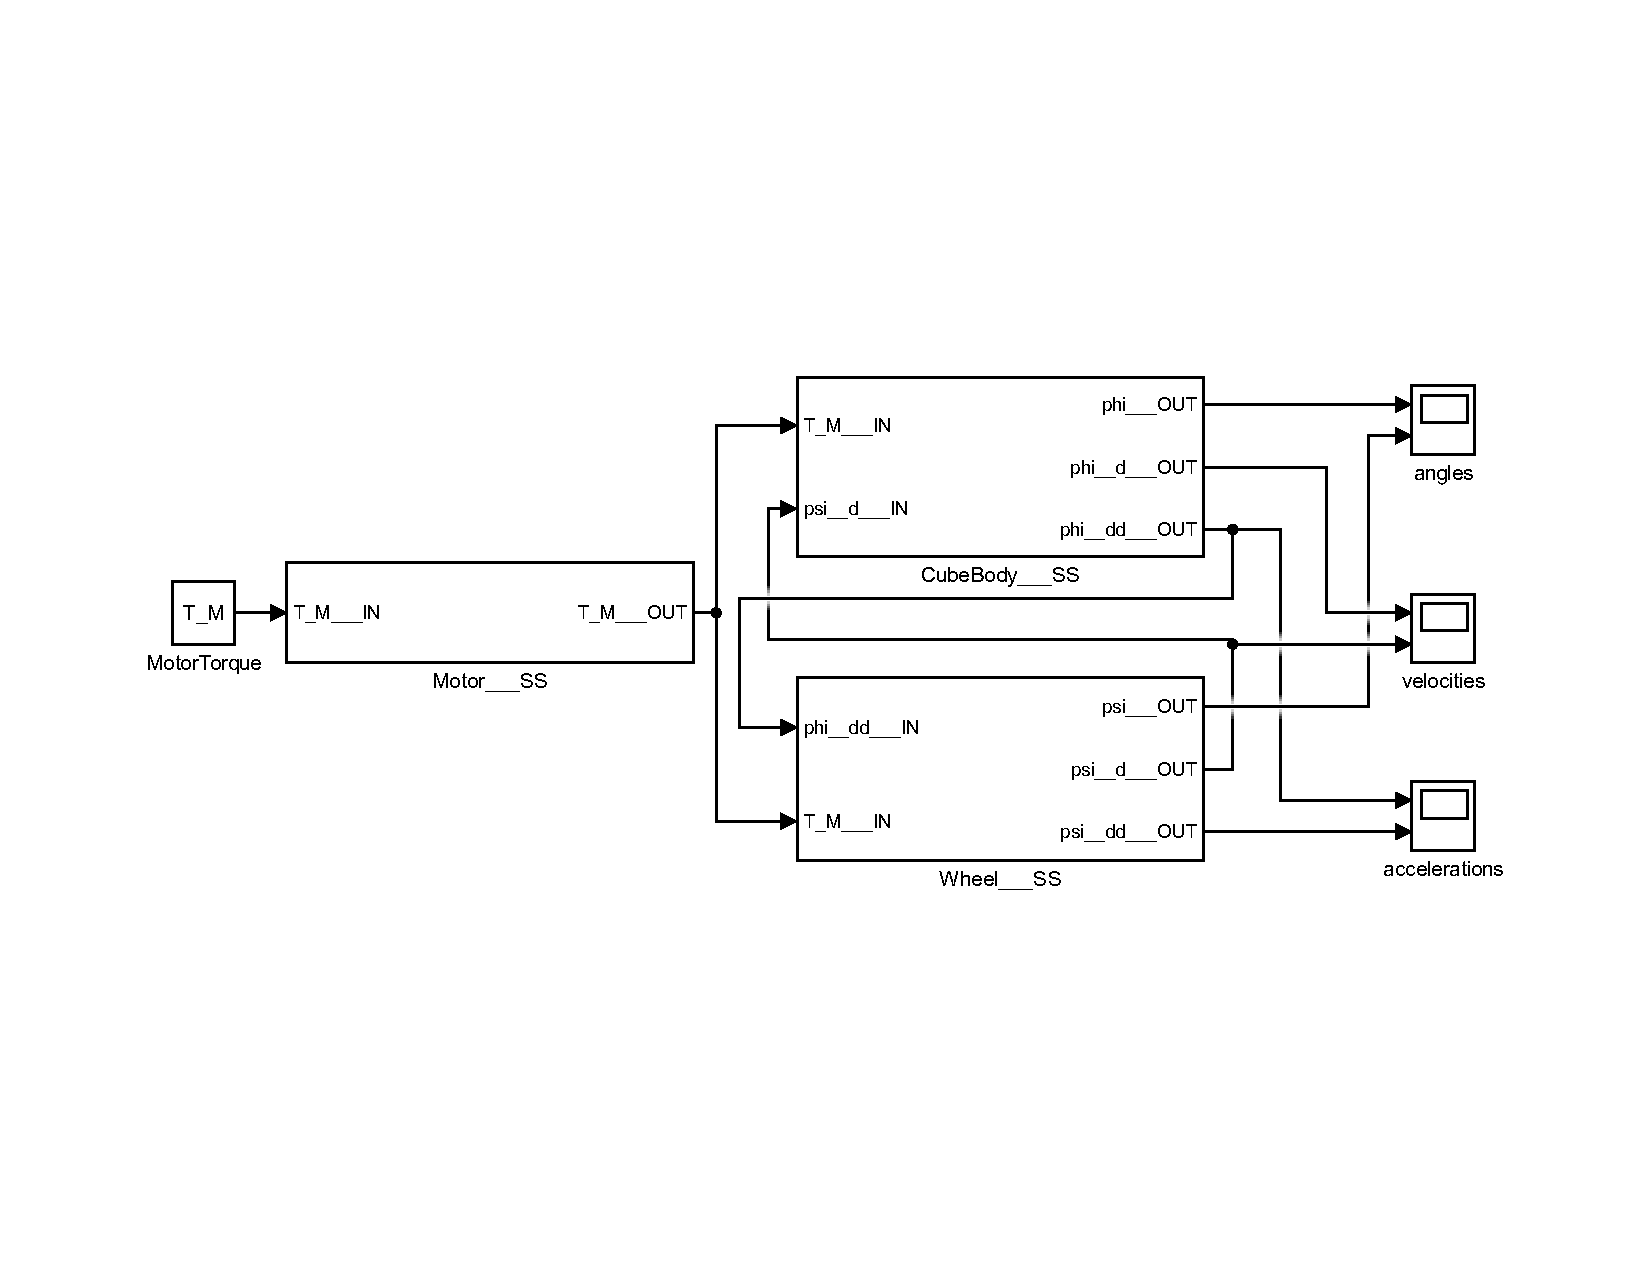
\includegraphics[width=\linewidth, trim={0 7cm 0 6cm},clip]{model_1D_overview}
\caption{Simulink-Modell Übersicht, Quelle: eigene Darstellung}
\end{figure}

\subsubsubsection{Simulation des Motors}
Der Motor wird als zwei in Reihe geschaltete PT1-Glieder simuliert. Da der Regler als Stellgröße ein Motormoment berechnet, beträgt die Verstärkung des Motor $K_M$ in der Simulation den Wert eins. Die Zeitkonstanten der PT1-Glieder sind einerseits die elektrische Zeitkonstante $T_e$ und die mechanische Zeitkonstante $T_m$, wessen Werte dem Datenblatt des Herstellers entnommen werden.

\begin{equation}
K_M = 1 \hspace{35pt} T_e = 0.55ms \hspace{35pt} T_m = 12.4ms
\end{equation}

\subsubsubsection{Simulation der Würfelseite}
Die Dynamik der Würfelseite wird von \ref{BG_phi_quation} beschrieben.

\begin{equation}
\ddot{\varphi} = \frac{g(m_R \cdot l_{AB}^2 + m_K \cdot l_{AC})sin(\varphi) - C_{\varphi} \cdot \dot{\varphi} + C_{\psi} \cdot \dot{\psi} - T_M}{{\theta}^A_K + m_R \cdot l_{AB}^2} \tag{\ref{BG_phi_quation}}
\end{equation}

Somit ist die Winkelbeschleunigung gleich der Summe der Drehmomente geteilt durch die betroffenen Massenträgheitsmomente. Durch Integration und Rückführung können die einzelnen Drehmomente berechnet werden. Das folgende Modell zeigt die Umsetzung dieser Berechnungsvorschrift in Simulink.

\begin{figure}[h]
\label{Simulink_1DModell_CubeBody_pic}
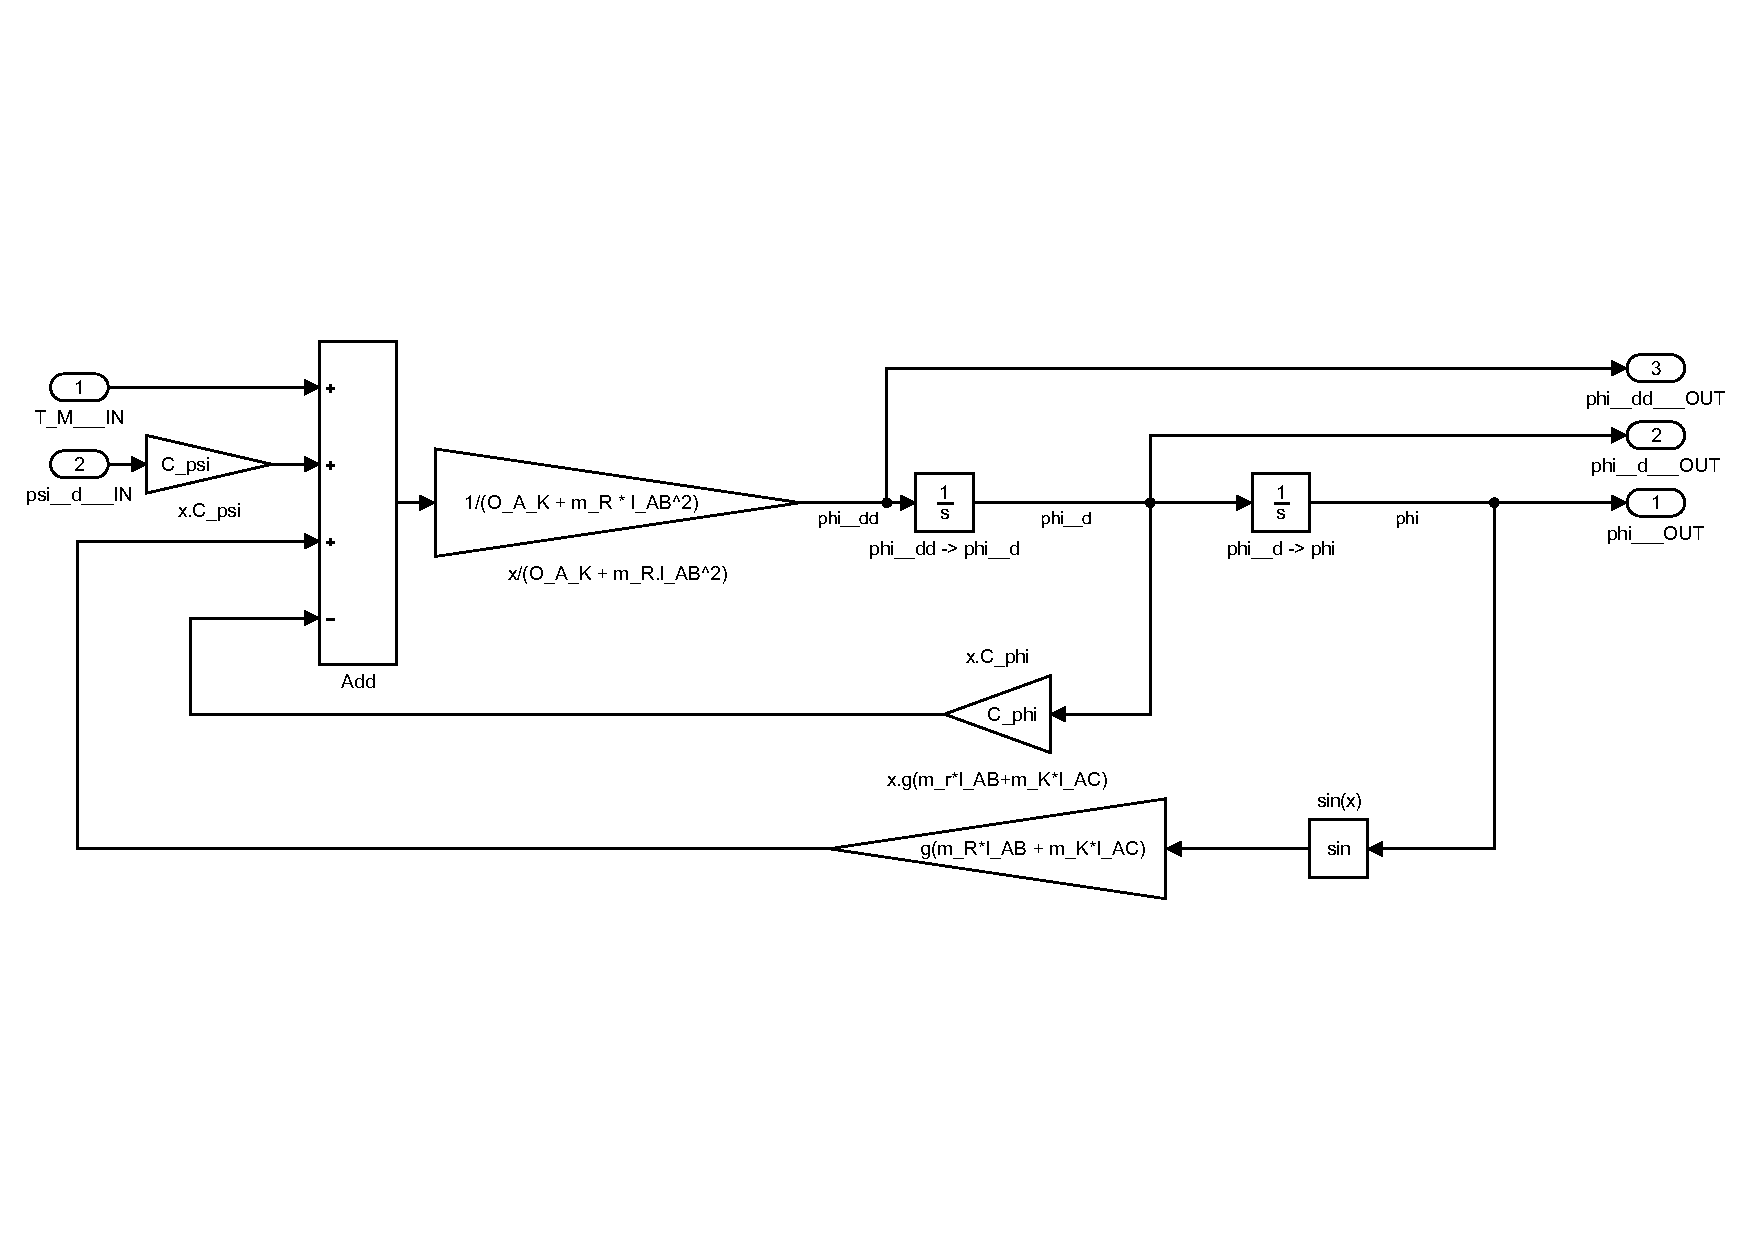
\includegraphics[width=\linewidth, trim={0 5cm 0 5cm},clip]{model_1D_cubebody}
\caption{Subsystem Würfelseite, Quelle: eigene Darstellung}
\end{figure}

\subsubsubsection{Simulation der Schwungmasse}
Die Dynamik der Schwungmasse wird von \ref{BG_psi_equation} beschrieben, allerdings wird das Modell vereinfacht indem $\ddot{phi}$ nicht substituiert wird.

\begin{equation}
{\theta}^R_B \cdot \ddot{\psi} = T_M - C_{\psi} \cdot \dot{\psi} - {\theta}^B_R \cdot \ddot{\varphi}\tag{\ref{BG_psi_equation}}
\end{equation}

Das Simulink-Modell folgt dem selben Schema wie das Subsystem zur Simulation der Bewegung des Würfelkörpers.

\begin{figure}[h]
\label{Simulink_1DModell_Wheel_pic}
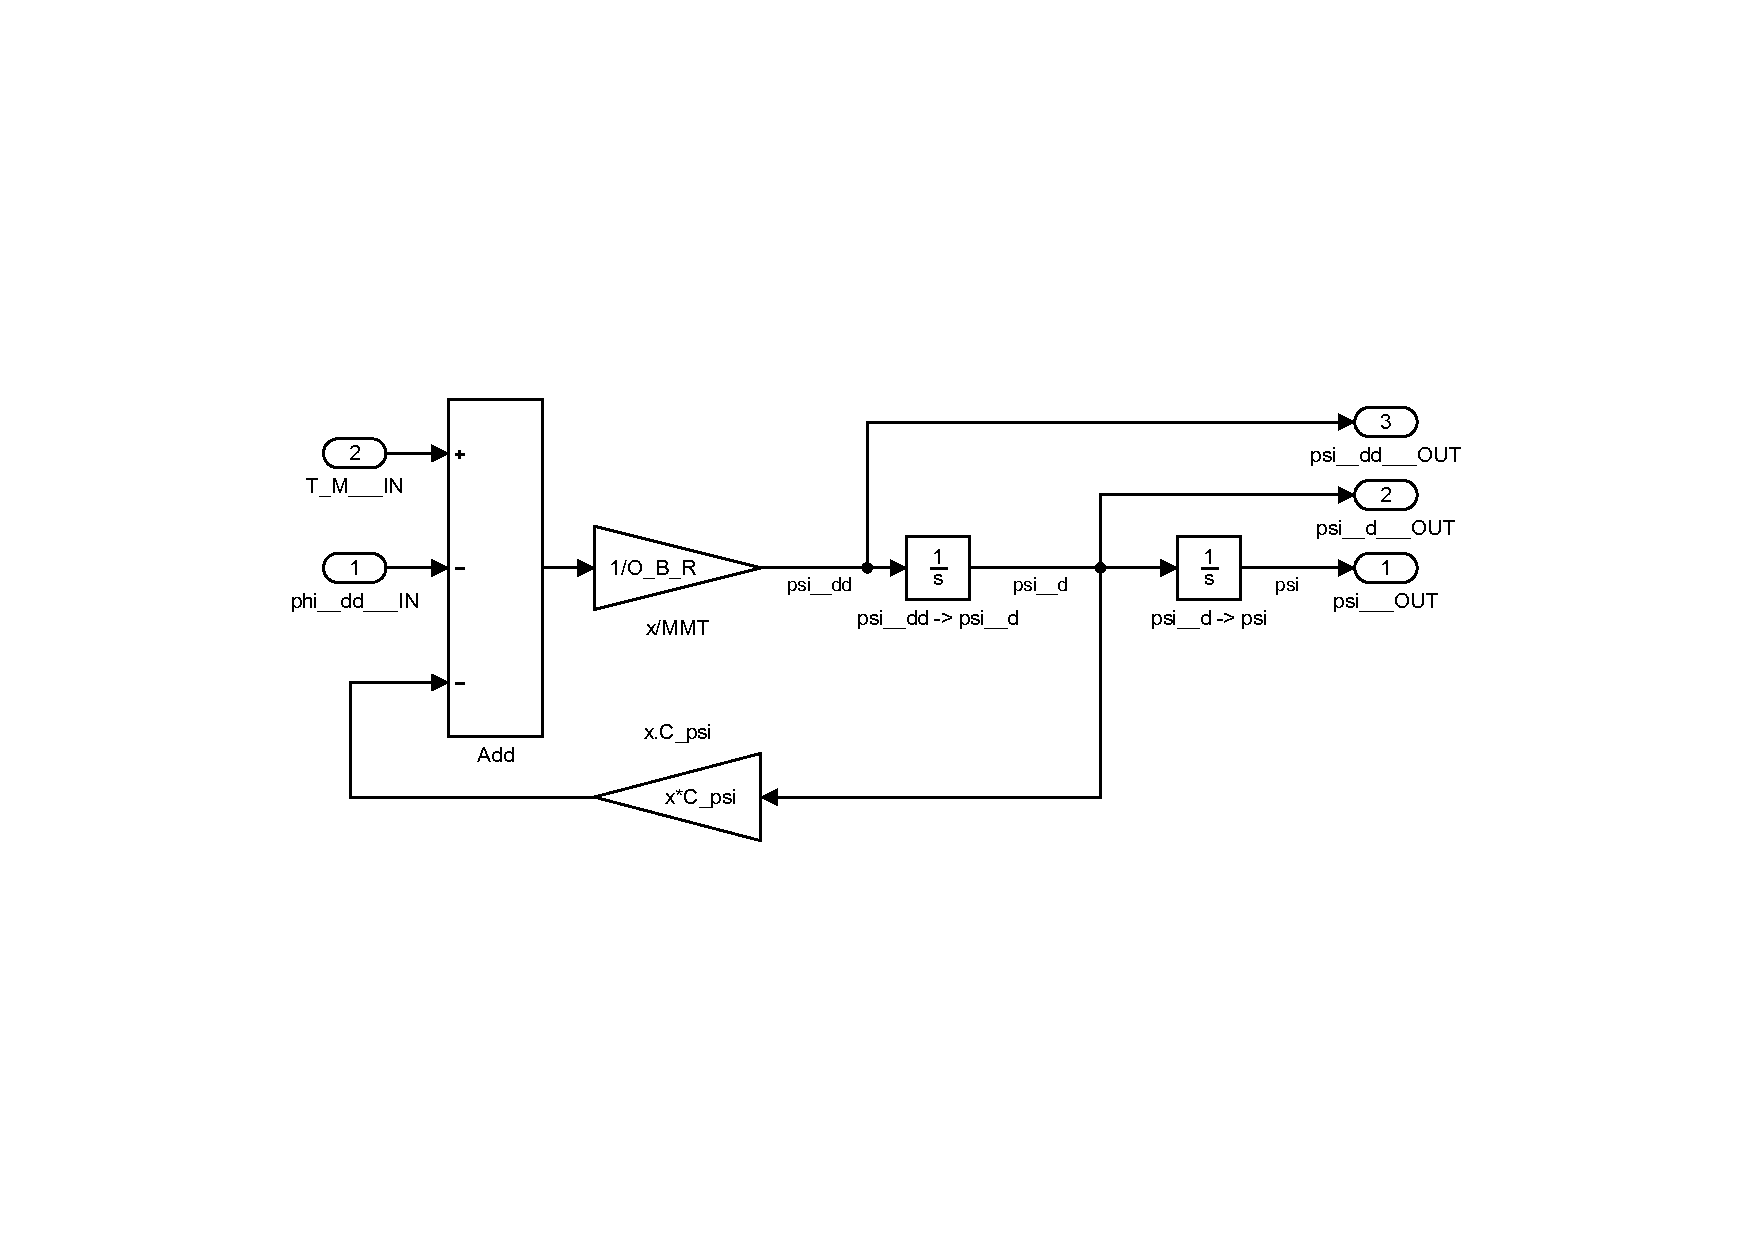
\includegraphics[width=\linewidth, trim={0 6cm 0 6cm},clip]{model_1D_wheel}
\caption{Subsystem Schwungmasse, Quelle: eigene Darstellung}
\end{figure}
\subsection{Reglerentwurf}
In dem folgenden Abschnitt wird der Entwurf eines Reglers vorgestellt, welcher auf der Rückführung des Zustandsvektors basiert. Im ersten Teil wird die analytische Bestimmung der Parameter erläutert, daraufhin wird der Regler im zweiten Teil an dem Prototyp erprobt und validiert.

\subsubsection{Analytische Bestimmung der Reglerparameter}
Mit Hilfe der Zustandsraumdarstellung kann über die Rückführung des Zustandvektors eine Regelung entworfen werden. Das folgende Blockschaltbild zeigt den Zusammenhang der Systemmatrizen und der Reglermatrix $\textbf{F}$, welche zur Berechnung der Stellgröße $u=T_M$ dient.

\begin{figure}[h]
\label{Regelkreis_pic}
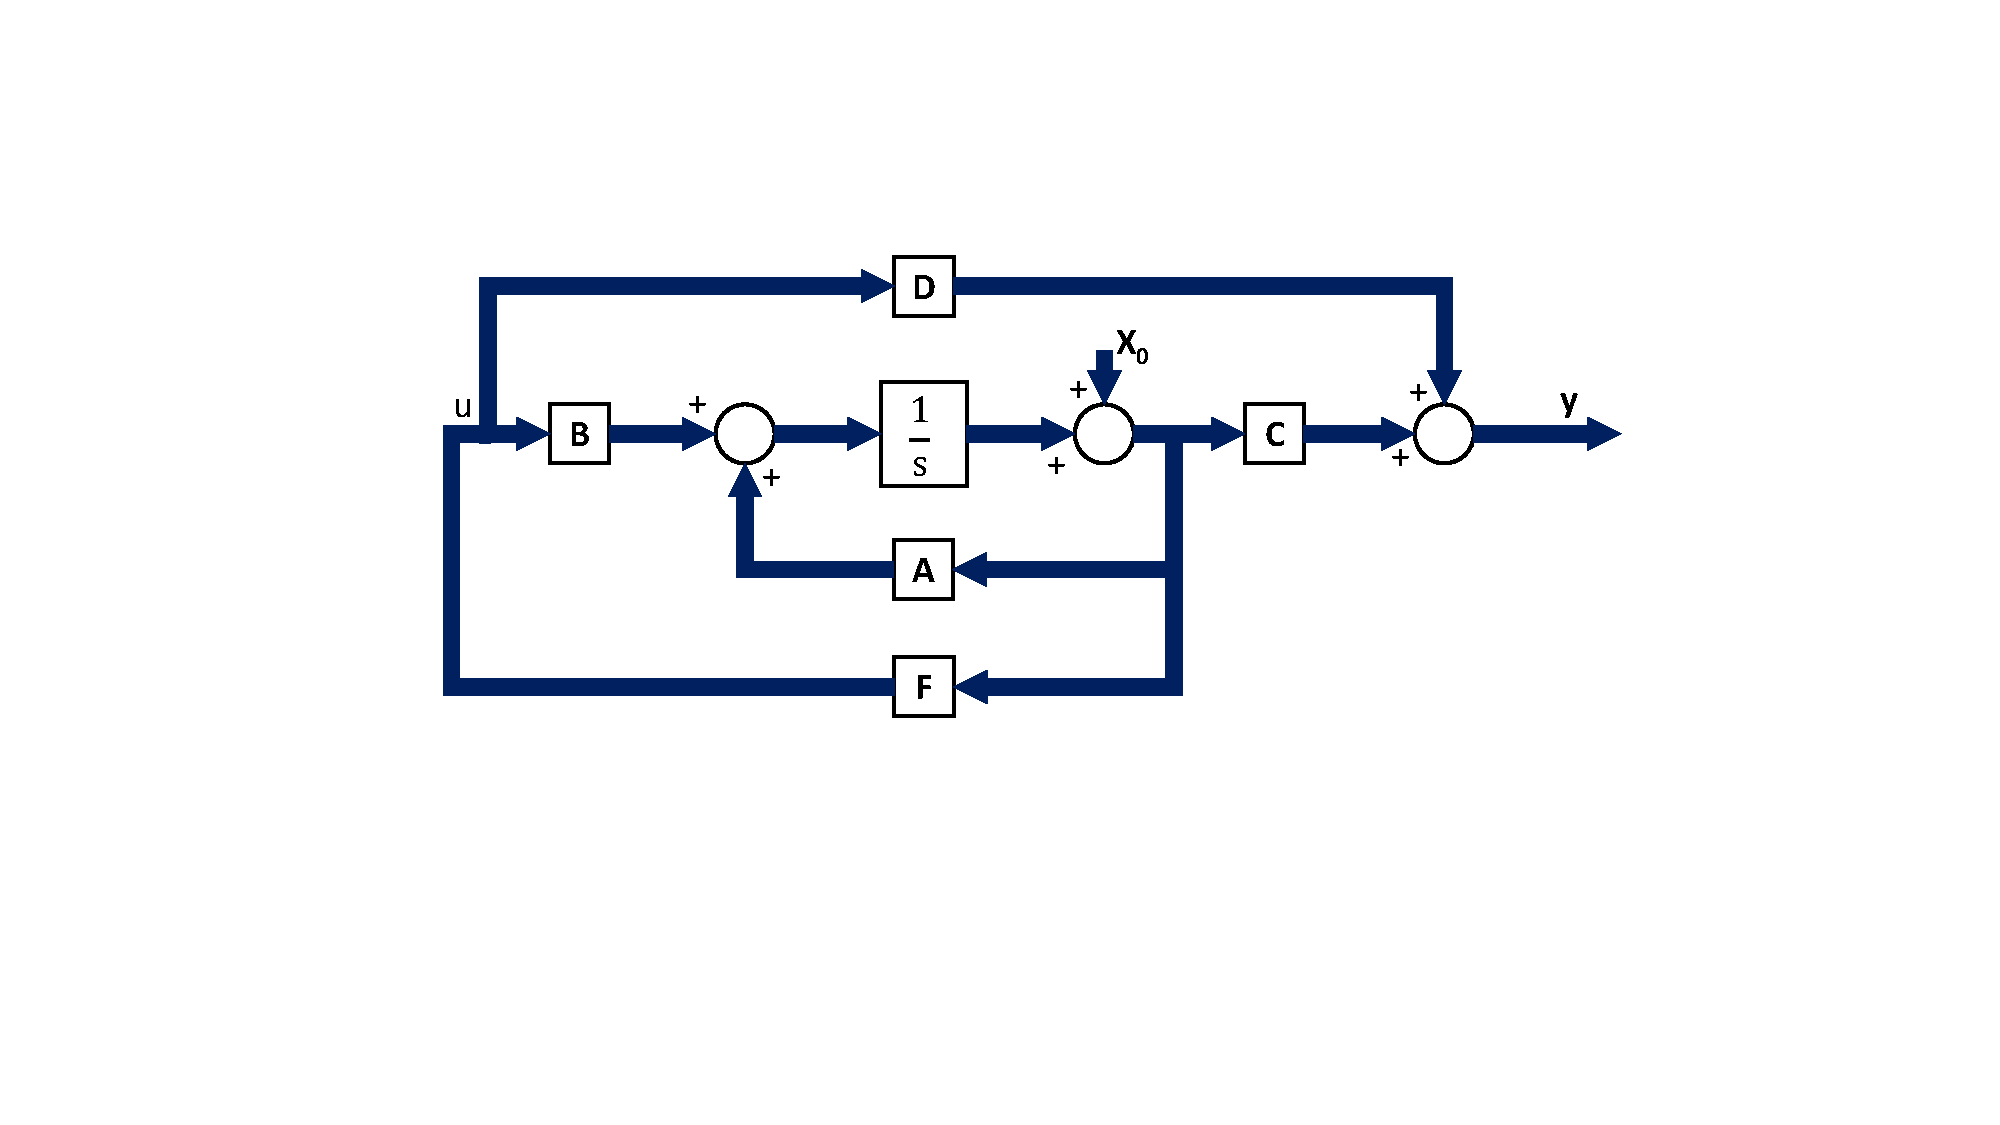
\includegraphics[width=\linewidth, trim={0 6.5cm 0 3.5cm}, clip]{Bilder_RT}
\caption{Blockschaltbild Regelkreis, Quelle: eigene Darstellung, Inhalt aus \cite{RT2}}
\end{figure}

Die Stellgröße $u$ wird von einem Mikrokontroller mit einer Abtastperiod $T_a = 20ms$ berechnet. Folglich handelt es sich um eine digitale Regelung. Um das Verhalten des diskreten Systems zu beschreiben müssen die diskreten Systemmatrizen $\textbf{A}_d$, $\textbf{B}_d$, $\textbf{C}_d$ und $\textbf{D}_d$ berechnet werden. Hierfür gilt nach \cite{RT2}:

\begin{equation}
\textbf{S} = T_a \sum_{v=0}^{\infty} \textbf{A}^v \frac{T^v}{(v+1)!}
\end{equation}
\begin{equation}
\textbf{A}_d = \textbf{I} + \textbf{S} \cdot \textbf{A}
\end{equation}
\begin{equation}
\textbf{B}_d = \textbf{S} \cdot \textbf{B}
\end{equation}
\begin{equation}
\textbf{C}_d = \textbf{C}
\end{equation}
\begin{equation}
\textbf{D}_d = \textbf{D}
\end{equation}

Die Reglermatrix $\textbf{F}$ wird als optimaler Zustandsregler nach dem quadratischen Gütekriterium entworfen. Die diskrete Gütefunktion für dieses System lautet:

\begin{equation}
\label{costfunction_equation}
I = \sum_{k=1}^\infty \textbf{x}^T(k) \cdot \textbf{Q} \cdot \textbf{x}(k) + R\cdot u(k)^2
\end{equation}

Die Matrizen $\textbf{Q}$ und $\textbf{R}$ stellen Gewichtungen der Zustands- und Stellgrößen dar. Die Ausgangswerte dieser Matrizen werden mit der Faustformel nach (\cite{lqrnotes}) berechnet. Ggf. können die Werte anschließend angepasst werden um die Reglergüte weiter zu verbessern.

\begin{equation}
\textbf{Q} = \begin{pmatrix}
\frac{1}{(\varphi_{max})^2} & 0 & 0 \\
0 & \frac{1}{(\dot{\varphi}_{max})^2} & 0 \\
0 & 0 & \frac{1}{(\dot{\psi}_{max})^2} \\
\end{pmatrix}
\end{equation}
\begin{equation}
R = \begin{pmatrix}
\frac{1}{(T_{M,max})^2}
\end{pmatrix}
\end{equation}

Die Reglermatrix $\textbf{F}$ muss die Eigenschaft besitzen die Gütefunktion (\ref{costfunction_equation}) zu minimieren. Dieses Problem wird mit Hilfe von der Matlab-Funktion \textit{lqrd} numerisch gelöst.

\subsubsection{Verifizierung des Reglers an dem 1D-Prototyp}
Mit Hilfe von Matlab wurden die Werte der Reglermatrix $\boldsymbol{F}$ berechnet.

\begin{equation}
\boldsymbol{F} = \begin{pmatrix}
0.8821 & 0.1386 & 0.0002
\end{pmatrix}
\end{equation}

Somit lässt sich das Motormoment $T_{M,n}$ durch die Rückführung des Zustandvektors $\boldsymbol{x}_n$ über die Reglermatrix $\boldsymbol{F}$ berechnen.

\begin{equation}
T_{M,n} = \boldsymbol{F} \cdot \boldsymbol{x}_n
\end{equation}

Der Regler wird zuerst mit Hilfe eines Simulink-Modelles in der Simulation überprüft. Anschließend wird der geschlossene Regelkreis auf den Prototyp übertragen. Hierbei ist zu beachten, dass bei der Modellierung des Systemverhaltens die Annahme getroffen wurde, dass der Schwerpunkt des Systems auf dessen Y-Achse liegt. Durch den unsymmetrischen Aufbau ist dies allerdings nicht der Fall, somit ergibt sich das folgende Gravitationsmoment  $M_G$, wobei der Winkel $\varphi_{cog}$ den Winkel zwischen Y-Achse und Schwerpunkt der Würfelseite bezeichnet.

\begin{equation}
M_G = g(m_K \cdot l_{AC} + m_R \cdot l_{AB}) \cdot sin(\varphi + \varphi_{cog})
\end{equation}

Somit muss ein konstantes Motormoment erzeugt werden, um die Würfelseite bei dem Sollwinkel $\varphi = 0$ zu halten. Dadurch wird die Schwungmasse konstant beschleunigt, weshalb die Schwungmasse nicht vollständig zum Stillstand kommen kann. Deshalb muss für die Berechnung des Drehmomentes der Winkel $\varphi_{cog}$ zu der Zustandsgröße $\varphi$ addiert werden.

\begin{equation}
T_{M,n} = \boldsymbol{F} \cdot \begin{pmatrix}
\varphi + \varphi_{cog} \\
\dot{\varphi} \\
\dot{\psi}
\end{pmatrix}
\end{equation}

Da die Winkelgeschwindigkeit der Schwungmasse $\dot{\psi}$ nur dann verschwindet wenn das Motormoment gleich null ist, kann der Wert von $\varphi_{cog}$ empirisch ermittelt werden.


\subsection{Aufspringen}
Das Aufspringen der Würfelseite wird durch das abrupte bremsen der Schwungmasse ermöglicht. Hierbei wird der Drehimpuls der Schwungmasse auf das Gesamtsystem übertragen. Dieser Vorgang kann als nicht elastischer Stoß modelliert werden. Somit ergibt sich aus dem Drehimpulserhaltungssatz folgende Gleichung, wobei $\dot{\varphi}_B$ die Winkelgeschwindigkeit der Würfelseite nach dem Bremsen und $\dot{\psi}_B$ die Winkelgeschwindigkeit der Schwungmasse vor dem Bremsen darstellt.

\begin{equation}
\label{impulserhaltung_bremsen_equation}
(\theta^A_K + \theta^B_R + m_R \cdot l_{AB}) \cdot \dot{\varphi}_B = \theta^B_R \cdot \dot{\psi}_B
\end{equation} 

Um die Würfelseite von der Ruhelage ($\varphi_R = \pm \frac{\pi}{4}$) zu dem Gleichgewichtspunkt ($\varphi_G = 0$) zu bewegen muss Arbeite verrichtet werden. Diese Arbeit $W$ ist gleich der Änderung der potentiellen Energie von der Ruhelage hin zu dem Gleichgewichtspunkt.

\begin{equation}
\label{arbeit_bremsen_equation}
W = V(\varphi_G) - V(\varphi_R) = g(m_K + m_R) l_{AC} \cdot (cos(\varphi_G) - cos(\varphi_R))
\end{equation}

Auf Grund des Energieerhaltungssatzes muss die kinetische Energie des Gesamtsystemes nach dem Bremsvorgang gleich der zu leistenden Arbeit sein um die Würfelseite aufzurichten. Somit kann der Zusammenhang von $\dot{\varphi}_B$ und der Arbeit $W$ wie folgt beschrieben werden.

\begin{equation}
\label{energie_bremsen_equation}
\frac{1}{2}(\theta^A_K + \theta^B_R + m_R \cdot l_{AB}) \dot{\varphi}_B^2 = g(m_K + m_R) l_{AC} \cdot (1 - \frac{1}{\sqrt{2}})
\end{equation}

Mit Hilfe der Gleichungen (\ref{energie_bremsen_equation}) und (\ref{impulserhaltung_bremsen_equation}) kann nun die notwendige Bremsgeschwindigkeit $\dot{\psi}_B$ berechnet werden.

\begin{equation}
\label{psi_bremsen_equation}
\dot{\psi}_B = \sqrt{(2-\sqrt{2}(m_R + m_K) \cdot l_{AC} \cdot g \cdot \frac{\theta^A_K + \theta^B_R + m_R \cdot l_{AB}}{{\theta^B_R}^2}}
\end{equation}

Das obige Modell geht von der Annahme aus, dass es sich um einen perfekt nicht elastischen Stoß handelt und bei der Bewegung der Würfelseite keine Energie verloren geht. Somit besteht eine Abweichung des Modells von den realen Bedingungen. Um diese Abweichungen zu minimieren wird ein, an den Gradientenabstieg angelehnter, Lernalgorithmus implementiert. Nach dem Abbremsen der Schwungmasse werden die Größen $\varphi$ und $\dot{\varphi}$ beobachtet. Tritt ein Nulldurchgang von $\varphi$ auf bedeutet dies, dass die Anfangsgeschwindigkeit $\dot{\varphi}_B$ und somit die Radgeschwindigkeit $\dot{\psi}_B$ zu hoch waren. Tritt jedoch ein Nulldurchgang von $\dot{\varphi}$ auf, folgt, dass $\dot{\varphi}_B$ und $\dot{\psi}_B$ zu niedrig waren. In beiden Fällen kann die Änderung der Energie $\Delta E$, welche nötig ist um den Zielpunkt zu erreichen, berechnet werden.

\begin{equation}
\Delta E = \begin{cases}
\begin{matrix}
(1-cos(\varphi_0))(m_K+m_r)l_{AC} \cdot g  & \hspace{35pt} \vert \hspace{5pt} \dot{\varphi} = 0 \\
-\frac{1}{2}(\theta^A_K + \theta^B_R + m_R \cdot l_{AB}) \cdot \dot{\varphi}^2_0 & \hspace{35pt} \vert \hspace{5pt} {\varphi} = 0 \\
\end{matrix}

\end{cases}
\end{equation}

Mit Hilfe der Drehimpuls- (\ref{impulserhaltung_bremsen_equation}) und Energieerhaltung (\ref{energie_bremsen_equation} wird nun aus der Energieänderung $\Delta E$ die nötige Änderung der Radgeschwindigkeit $\Delta \dot{\psi}_B$ berechnet.

\begin{equation}
\pm \Delta \dot{\psi}_B = \sqrt{2 \cdot \frac{\theta^A_K + \theta^B_R + m_R \cdot l_{AB}}{{\theta^B_R}^2} \cdot \Delta E}
\end{equation}

Die Konvergenz des Lernalgorithmus gegen den Zielwert wird empirisch bewiesen, hierfür ist allerdings das hinzufügen einer Lernrate $\mu$ erforderlich. Daraus ergibt sich letztendlich folgende Vorschrift um den aktuellen Wert der Bremsgeschwindigkeit $\dot{\psi}_B$ zu bestimmen.

\begin{equation}
\dot{\psi}_B := \dot{\psi}_B + \mu \cdot \Delta \dot{\psi}_B \hspace{35pt} \vert \hspace{5pt} 0 < \mu \le 1
\end{equation}
\subsection{Software}
Im folgenden wird die Ansteuerung und Auswertung der elektrischen Komponenten näher beschrieben. Außerdem wird die Kommunikation zwischen der Host- und Target-Plattform erläutert. Als Zielplattform wird ein \ac{BBB} verwendet, auf welchem eine Linux-Distribution ausgeführt wird. In der folgenden Abbildung sind die einzelnen Bausteine und deren Verbindung zu der Zielplattform dargestellt.

\begin{figure}[!h]
\centering
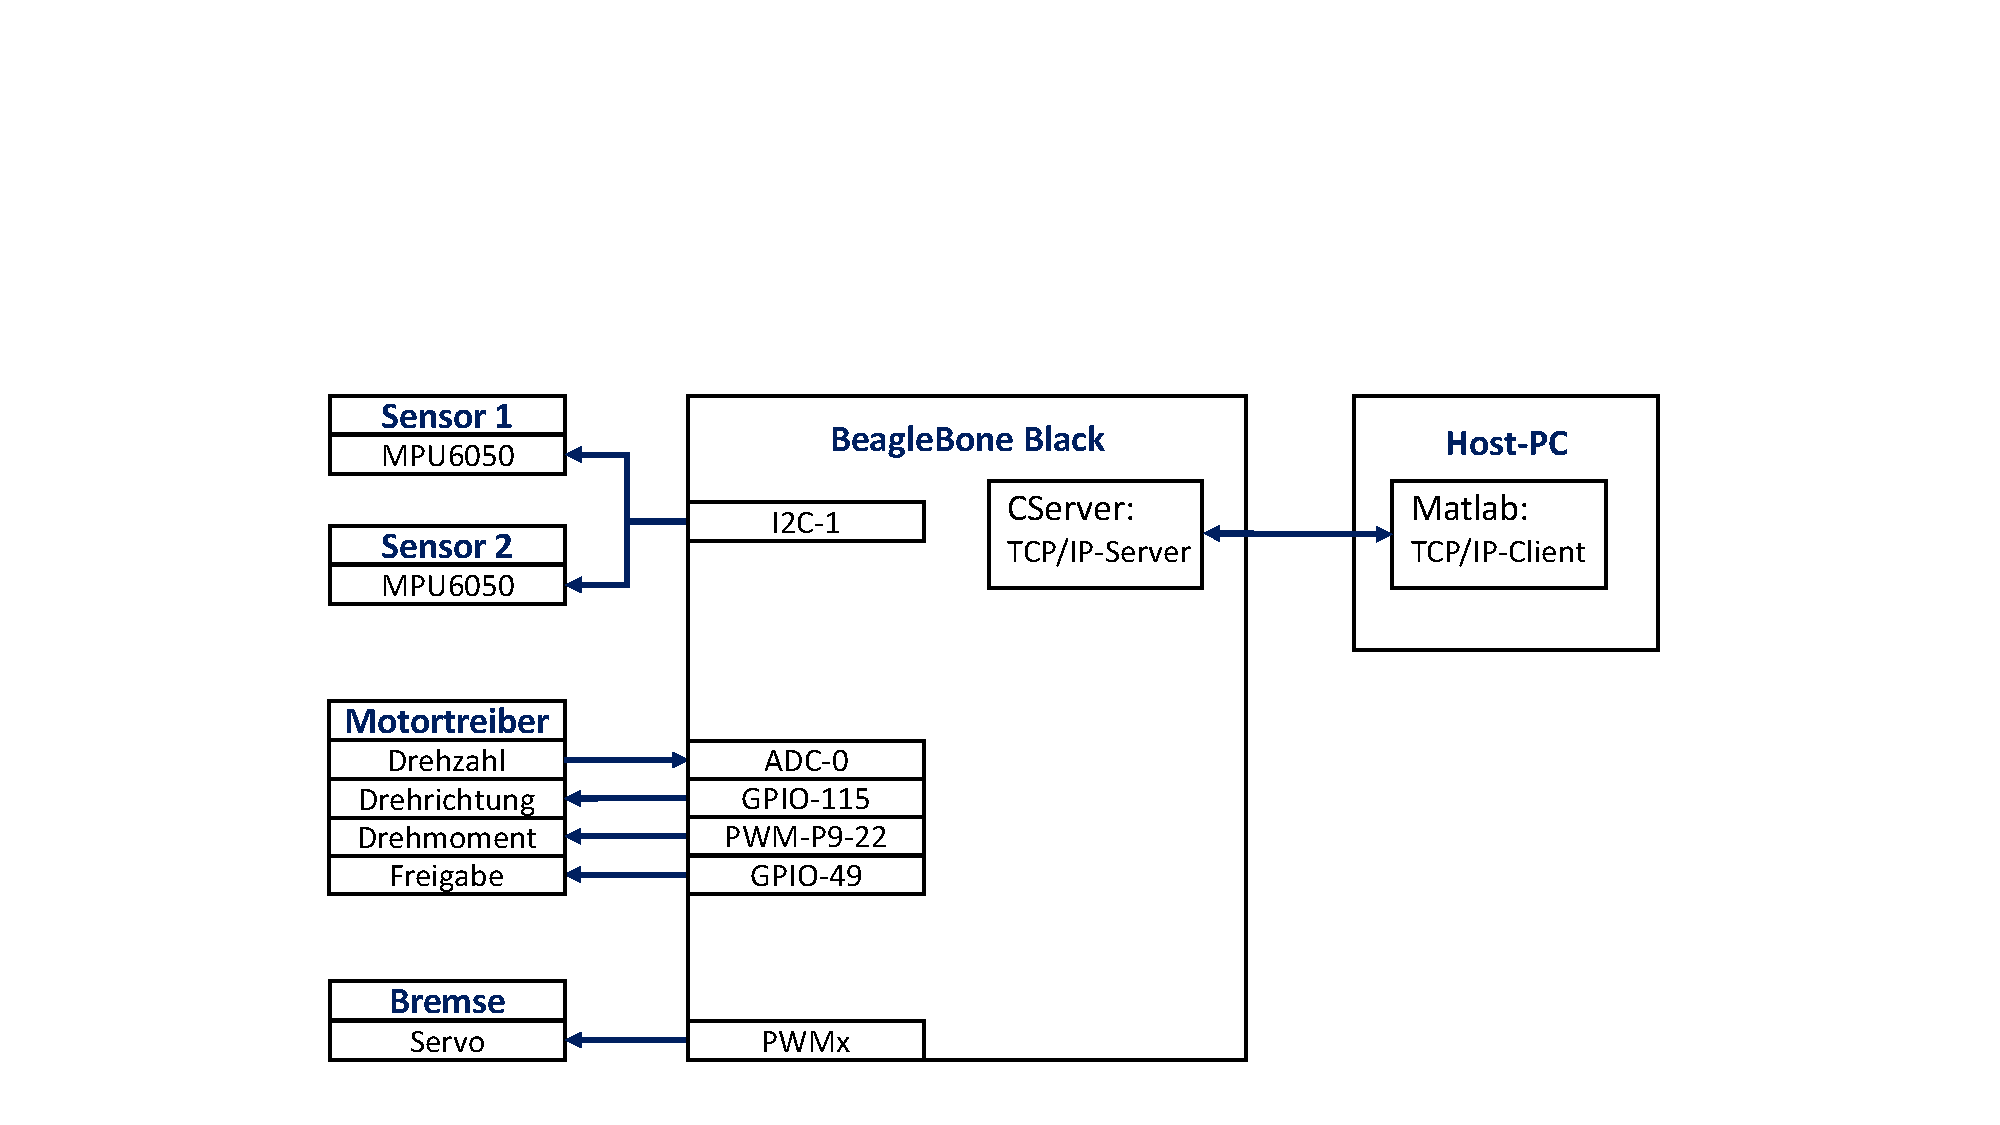
\includegraphics[width=0.8\linewidth, trim={4cm 1cm 5cm 6cm},clip]{img/ElekAufbau_Kommunikation}
\caption{Blockschaltbild der Komponenten, Quelle: eigene Darstellung}
\end{figure}

Um die verschiedenen Versuche und Messungen durchzuführen wird eine Software-Basis entworfen, welche als Grundlage für die verschiedenen Applikationen dient. Diese Grundlage umfasst eine objektorientierte Kapselung der Hardware, die TCP-Server-Implementierung um mit der MATLAB-Anwendung zu kommunizieren, die Definition zweier Komponenten, welche als separate Tasks ausgeführt werden und eine Kommunikationsstruktur für den Datenaustausch. Der Aufbau dieser Bausteine wird in den folgenden Abschnitten näher erläutert. Insgesamt werden acht Versuche durchgeführt:

\begin{itemize}
 \item V1: Bestimmung eines Ausgleichspolynoms um die Sensorwerte in SI-Einheiten umzurechnen. Hierfür werden die X- und Y-Beschleunigungswerte der beiden Sensoren benötigt.
 \item V2: Bestimmung des Offset der Gyroscopes. Hierfür werden die Z-Winkelgeschwindigkeiten der beiden Sensoren benötigt.
 \item V3: Bestimmung eines Ausgleichspolynoms um die ADC-Werte in SI-Einheiten umzurechnen. Hierfür werden die ADC-Werte der Motorgeschwindigkeit benötigt.
 \item V4: Test der Filter für $\varphi$, $\dot{\varphi}$ und ($\psi$). Hierfür müssen die verschiedenen Filter in SW realisiert werden.
 \item V5: Bestimmung des Reibwertes $C_{\varphi}$.
 \item V6: Bestimmung des Rebiwertes $C_{\psi}$.
 \item V7: Test und Bewertung des Regelkreises. Hierfür muss der Regelalgorithmus in SW realisiert werden.
 \item V8: Auspringen...
\end{itemize}

\subsubsection{Hardware-Schnittstelle}
Die Interaktion mit den Treibern des Betriebssystems wird mit Hilfe von Klassen gekapselt. Dadurch entsteht eine einheitliche und benutzerfreundliche Schnittstelle zwischen Hard- und Software. Die Klasse zur Interaktion mit der Hardware muss das folgende Interface erfüllen.

\newpage
\begin{lstlisting}
class IHardware
{
public:
	virtual Int16 getX1__dd_raw() = 0;
	virtual Int16 getX2__dd_raw() = 0;
	virtual Int16 getY1__dd_raw() = 0;
	virtual Int16 getY2__dd_raw() = 0;
	virtual Int16 getPhi1__d_raw() = 0;
	virtual Int16 getPhi2__d_raw() = 0;
	virtual UInt16 getPsi__d_raw() = 0;
	virtual void openBrake() = 0;
	virtual void closeBrake() = 0;
	virtual void enableMotor() = 0;
	virtual void disableMotor() = 0;
	virtual void setTorque(const Float32 torque) = 0;
public:
	IHardware() = default;
	IHardware(const IHardware&) = delete;
	IHardware& operator=(const IHardware&) = delete;
	virtual ~IHardware() = default;
};

\end{lstlisting}

\subsubsection{TCP/IP-Verbindung}
Die Kommunikation zwischen der \ac{BBB}- und der MATLAB-Applikation verläuft über eine TCP/IP-Verbindung. Hierfür wird auf dem \ac{BBB} ein Server ausgeführt, welcher auf die Verbindungsanfrage des MATLAB-Clients wartet. Die Vorteile des gewählten Protokolls liegen einerseits in der gesicherten und abstrahierten Datenübertragung, andererseits in den anwendungsfreundlichen Bibliotheken für Linux und MATLAB. Mit Hilfe einer simulierten Ethernet-Verbindung über USB wird ein privates Netzwerk zwischen der Zielplattform und dem Entwiclungs-PC eingerichtet.

Bild mit Adressen/Socket, etc.

\subsubsection{Komponentenarchitektur}
Die Hauptaufgaben der Applikation werden auf zwei Komponenten verteilt. Die erste übernimmt die Auswertung der Sensorik, Berechnung der Filter- und Regelalgorithmen und Ansteuerung der Aktorik. Hierfür werden Klasen eingeführt um die verschiedenen Teilaufgaben getrennt zu bearbeiten und einen übersichtlichen Software-Entwurf zu erhalten. Die Hauptaufgabe der zweiten Komponente besteht in der Kommunikation mit der MATLAB-Applikation, welche mit Hilfe eines TCP/IP-Servers erfolgt. 
Die beiden Komponenten werden von einer abstrakten Basisklasse abgeleitet und in eigenständigen Prozessen ausgeführt. In der Elternklasse werden rein virtuelle Methoden festgehalten welche zur Initialisierung und Durchführung der verschiedenen Versuche dienen. Somit ist es möglich die Grundstruktur für die mehreren Applikationen wiederzuverwenden. Auf Grund der simplen Abläufe genügt ein Flag um wiederzugeben ob sich eine Komponente im \textit{STANDBY}- oder \textit{RUNNING}-Zustand befinden. Für komplexere Anwendung kann an dieser Stelle ein vollständiger Zustandsautomat implementiert werden.

\begin{lstlisting}
class AComponentBase
{
public:
	virtual void init() = 0;
	virtual void run_V1_AusgleichsPolynomAccelerometer() = 0;
	virtual void run_V2_OffsetGyroscope() = 0;
	virtual void run_V3_AusgleichsPolynomMotorADC() = 0;
	virtual void run_V4_FilterTest() = 0;
	virtual void run_V5_BestimmungC_psi() = 0;
	virtual void run_V6_BestimmungC_phi() = 0;
	virtual void run_V7_RegelungTest() = 0;
public:
	AComponentBase(TQueue<Config::QueueSize>& rxQueue,
				   TQueue<Config::QueueSize>& txQueue,
				   bool initStandby);
	AComponentBase() = delete;
	AComponentBase(const AComponentBase&) = delete;
	AComponentBase& operator=(const AComponentBase&) = delete;
	virtual ~AComponentBase() = default;
protected:
	TQueue<Config::QueueSize>& mRxQueue;
	TQueue<Config::QueueSize>& mTxQueue;
	bool mStandbyState;
	UInt8 mPadding{};
};

\end{lstlisting}

Die Kommunikation der beiden Prozess auf dem \ac{BBB} erfolgt mit Hilfe von Nachrichten. Dieser werden mit Hilfe von Queues, welche im \ac{SHM} angelegt werden, zwischen den beiden Prozessen ausgetauscht. Zusätzlich wird dieselbe Nachrichtenstruktur verwendet um Daten zwischen dem \ac{BBB} und der MATLAB-Anwendung auszutauschen. Hierfür werden die Daten als Byte-Stream über die TCP/IP-Verbindung übertragen. 

\begin{figure}[!h]
\centering
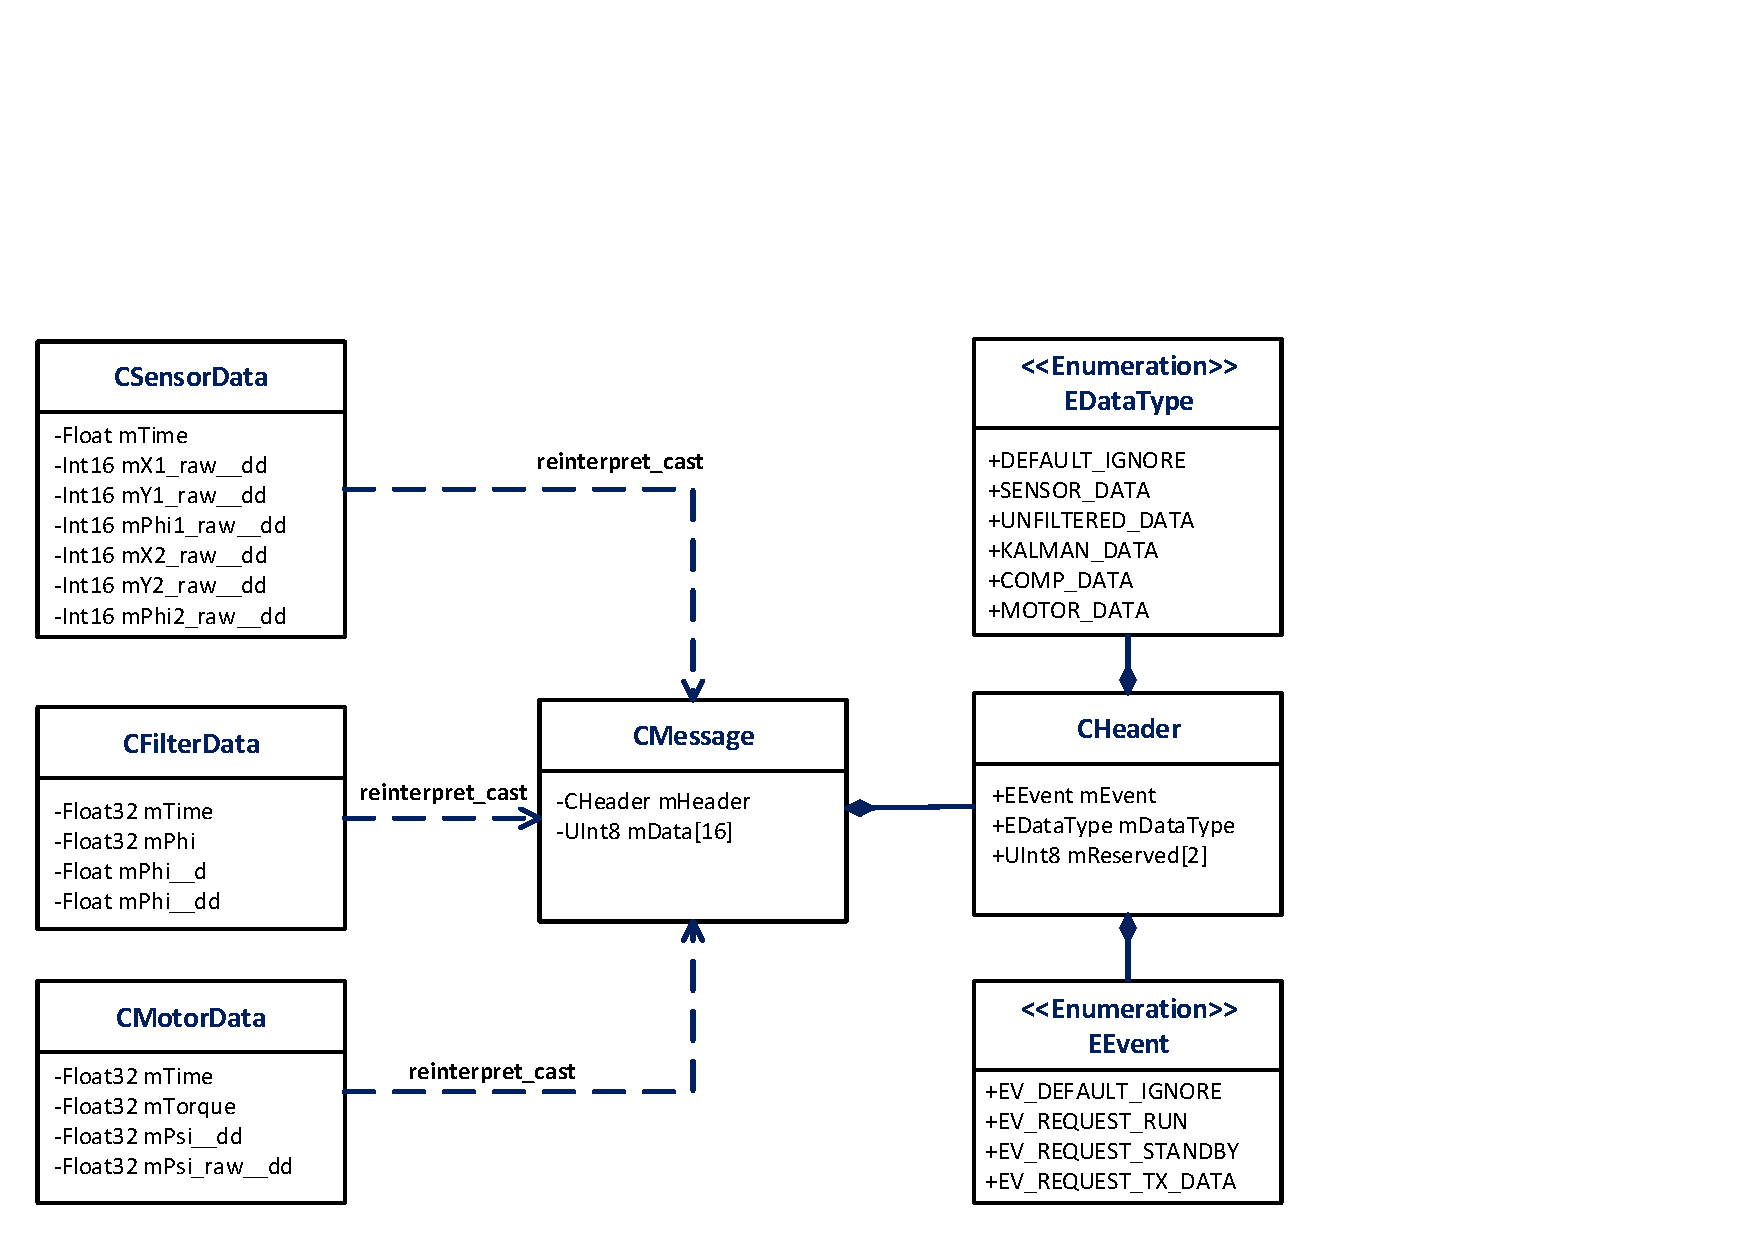
\includegraphics[width=0.8\linewidth, trim={0cm 0cm 7cm 5cm},clip]{img/UML_MessageClassDiag}
\caption{UML Nachrichtenaufbau, Quelle: eigene Darstellung}
\end{figure}

Die Nachrichten bestehen aus einem Header, welcher das Ereignis und weitere Informationen, wie z.B. den Typ der enthaltenen Daten. Das Datenfeld wird genutzt um relevante Informationen wie Sensor-, Filter- und Motorwerte an die MATLAB-Applikation zu übermitteln. Die Nachrichten werden in Form einer Klasse realisiert, welche Konstruktoren enthält um die verschiedenen Datenstrukturen in das Datenfeld zu legen.

\subsubsection{Allgemeiner Ablauf der Versuchsapplikationen}
Die Ablauf der unterschiedlichen Versuche ist auf Seite der SW sehr ähnlich. Die beiden Komponenten starten im \textit{STANDBY}-Zustand. Die Kommunikations-Komponente wartet darauf, dass der MATLAB-Client eine Verbindung aufbaut. Daraufhin wechselt diese in den \textit{RUNNING}-Zustand und sendet eine Nachricht an die \textit{Control}-Komponente, welche darauf ebenfalls in den \textit{RUNNING}-Zustand wechselt.
Im Anschluss wertet die \textit{Control}-Komponente in zyklischen Abständen die Sensoren aus, berechnet ggf. Filter- oder Reglerwerte und sendet diese mit Hilfe von Nachrichten an die Kommunikations-Komponente. Diese leitet empfangene Nachrichten an die MATLAB-Applikation weiter, welche diese virtualisiert und zur weiteren Verarbeitung speichert. 
Sobald die MATLAB-Anwendung die Verbindung abbricht wird eine entsprechende Nachricht an die \textit{Control}-Komponente gesendet. Daraufhin terminieren beide Prozesse selbständig.

\subsection{Ausblick}
Auf Grund des straffen Zeitplanes dieses Entwicklungsprojektes mussten einzelne Untersuchungen bzw. Erweiterungen vernachlässigt werden. Deshalb soll dieser Abschnitt einen Ausblick über mögliche Optimierungen schaffen, welche im Rahmen weiterer Projekte untersucht werden können. Eine der größten Herausforderungen hierbei waren die hohen Eigenfrequenzen des Systems die zu einem sehr dynamischen Verhalten führen. Dadurch sind simple Tiefpassfilter ungeeignet um Rauschsignale zu entfernen, da sie zu große Verzögerungen mit sich bringen. Auch der verwendete Regler muss in der Lage sein in kurzer Zeit auf Störungen zu reagieren.

Die verschiedenen Filter wurden in dieser Arbeit zum Teil nur oberflächlich untersucht, besonders der direkte Vergleich der Ansätze beruht lediglich auf dem Vergleich der letztendlichen Reglergüte. In diesem Bereich können weitere Verbesserungen erreicht werden in dem einerseits ein absolutes Referenzsignal gemessen wird um eine Bewertung der Filtersignale durchzuführen. Beispielsweise kann der Winkel $\varphi$ mit einem Drehgeber gemessen werden. Dadurch steht ein weiteres Signal zur Verfügung, das präziser als die Winkelschätzung bzw. die Filter ist und somit als Sollwert betrachtet werden kann. Weiterhin können die Rauschanteile der Sensorsignale näher untersucht werden um eine weitere Verbesserung der Filteralgorithem zu erreichen. Besonders das verwendete Komplementär-Filter verspricht hier großes Verbesserungspotential.

Außerdem wurde im Rahmen dieses Projektes lediglich ein Zustandsregler verwendet. Das Gebiet der Regelungstechnik bietet hier eine Vielzahl verschiedener Ansätze, welche eine zu weiteren Verbesserungen im Systemverhalten führen können. In dieser Hinsicht eignet sich das Projekt auch hervorragend als Testmittel um verschiedene Regler- und Filteralgorithmen miteinander zu vergleichen.

\section{3D-Modell}
Der zweite Teil des Projektes beschäftigt sich mit der Entwicklung des vollständigen Würfels (3D-Modell). Hierbei können die Ansätze des 1D-Modell übernommen werden, wobei deren Komplexität jedoch zunimmt. Beispielsweise werden aus den zwei Freiheitsgraden der Würfelseite sechs Freiheitsgrade für das 3D-Modell. Folglich steigt der Umfang der Systemanalyse und des Regelkreises. Eine besondere Schwierigkeit besteht darin, dass die drei Eingangsgrößen alle Systemzustände beeinflussen und somit nicht getrennt betrachtet werden können. Auch die Schätzung der Zustände mit Hilfe der Sensorwerte nimmt zu da sich die Anzahl der Sensorsignale verdreifacht und komplexere Beziehungen zwischen den Sensorwerten und den Systemzuständen bestehen.

Die Vorgehensweise ist dennoch identisch zu dem 1D-Modell, allerdings wird gezielt auf die Unterschiede zwischen den beiden Modellen eingegangen und Ergebnisse aus vorhergehenden Analyse als bekannt angenommen.

\begin{figure}[h!]
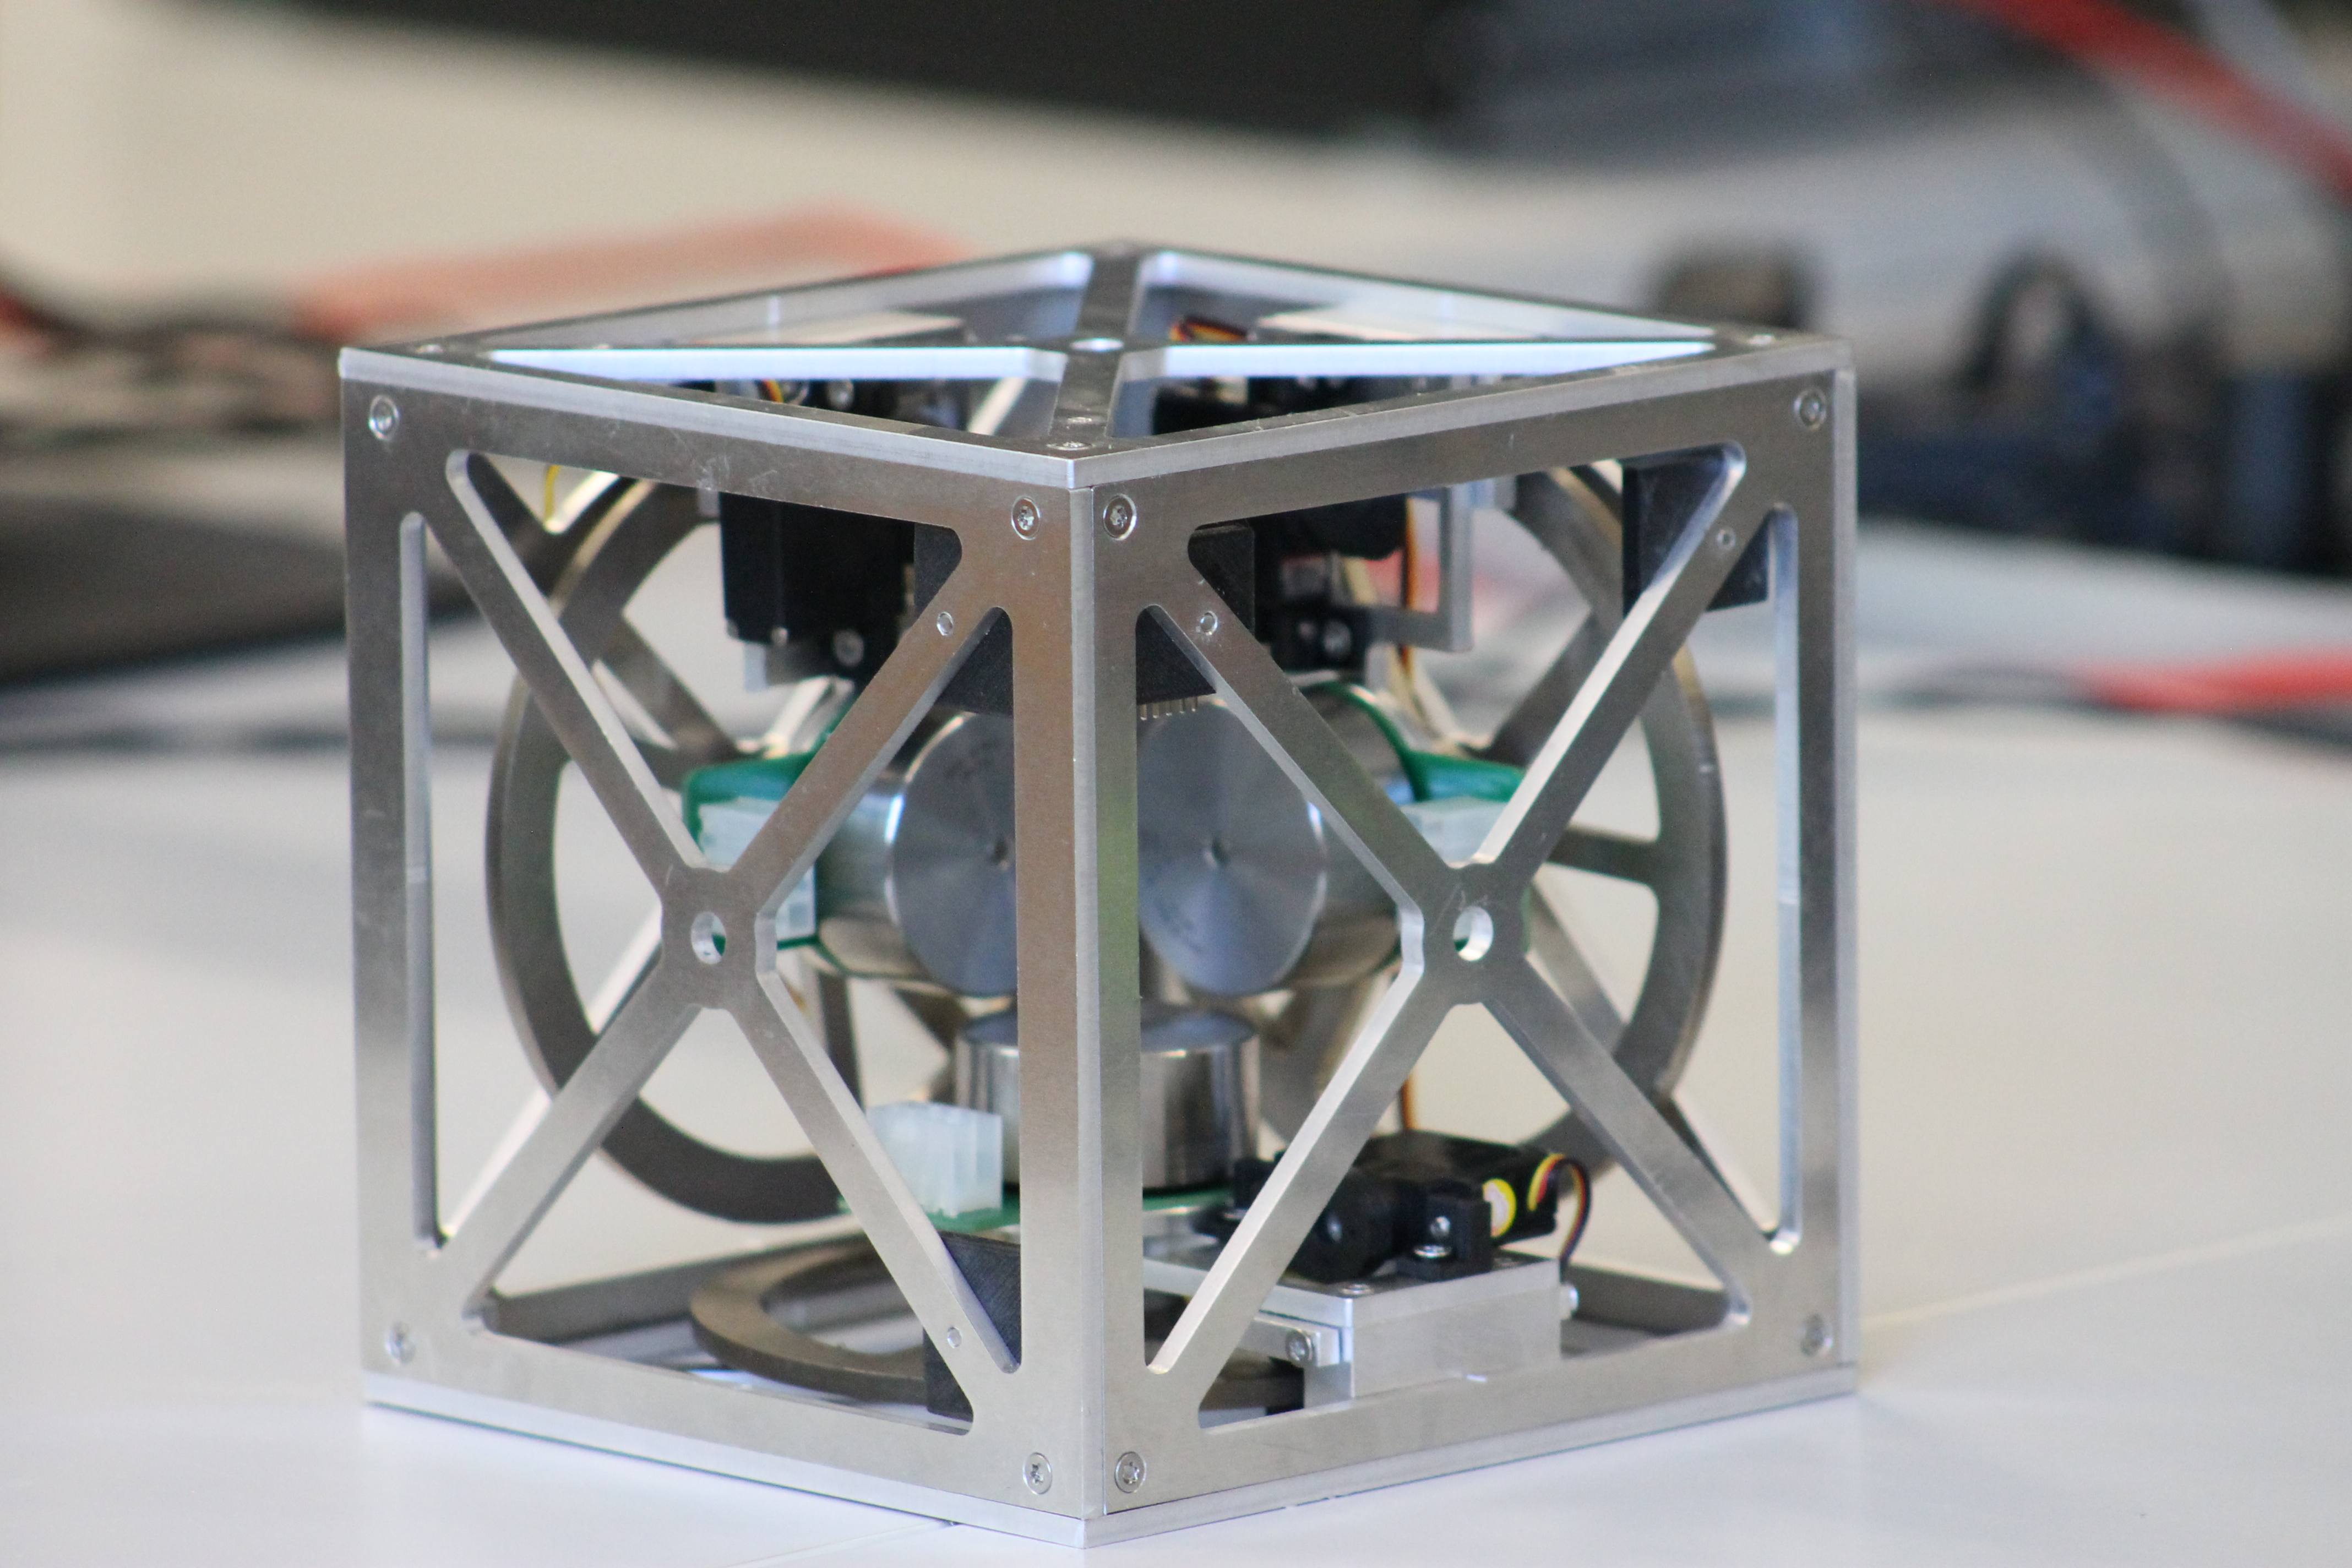
\includegraphics[width=\linewidth]{img/3D_Modell_img.JPG}
\caption{3D-Modell, Quelle: eigene Darstellung}
\end{figure}
\subsection{Modellierung der Systemdynamik}
In diesem Abschnitt werden die Bewegungsgleichungen des 3D-Modells mit Hilfe des Lagrange-Formalismus hergeleitet. Der Würfelkörper besitzt drei rotatorische Freiheitsgrade, die drei Schwungmassen verfügen über jeweils einen Freiheitsgrad. Somit ergeben sich insgesamt sechs Freiheitsgrade für das Gesamtsystem. Dadurch steigt die Komplexität der Systemdynamik stark an, allerdings bestehen nach wie vor Parallelen zu der Dynamik des 1D-Modells.
\newline

Um die Position des Würfels zu beschreiben wird ein raumfestes Bezugssystem $\{I\}$ eingeführt, welches von den drei Einheitsvektoren $\inI e_x$, $\inI e_y$ und $\inI e_z$ beschrieben wird. Das zweite Bezugssystem $\{W\}$ ist körperfest und rotiert somit mit dem Würfel. Es wird von den Einheitsvektoren $\inW e_x$, $\inW e_y$ und $\inW e_z$ beschrieben.

\begin{figure}[h]
\centering
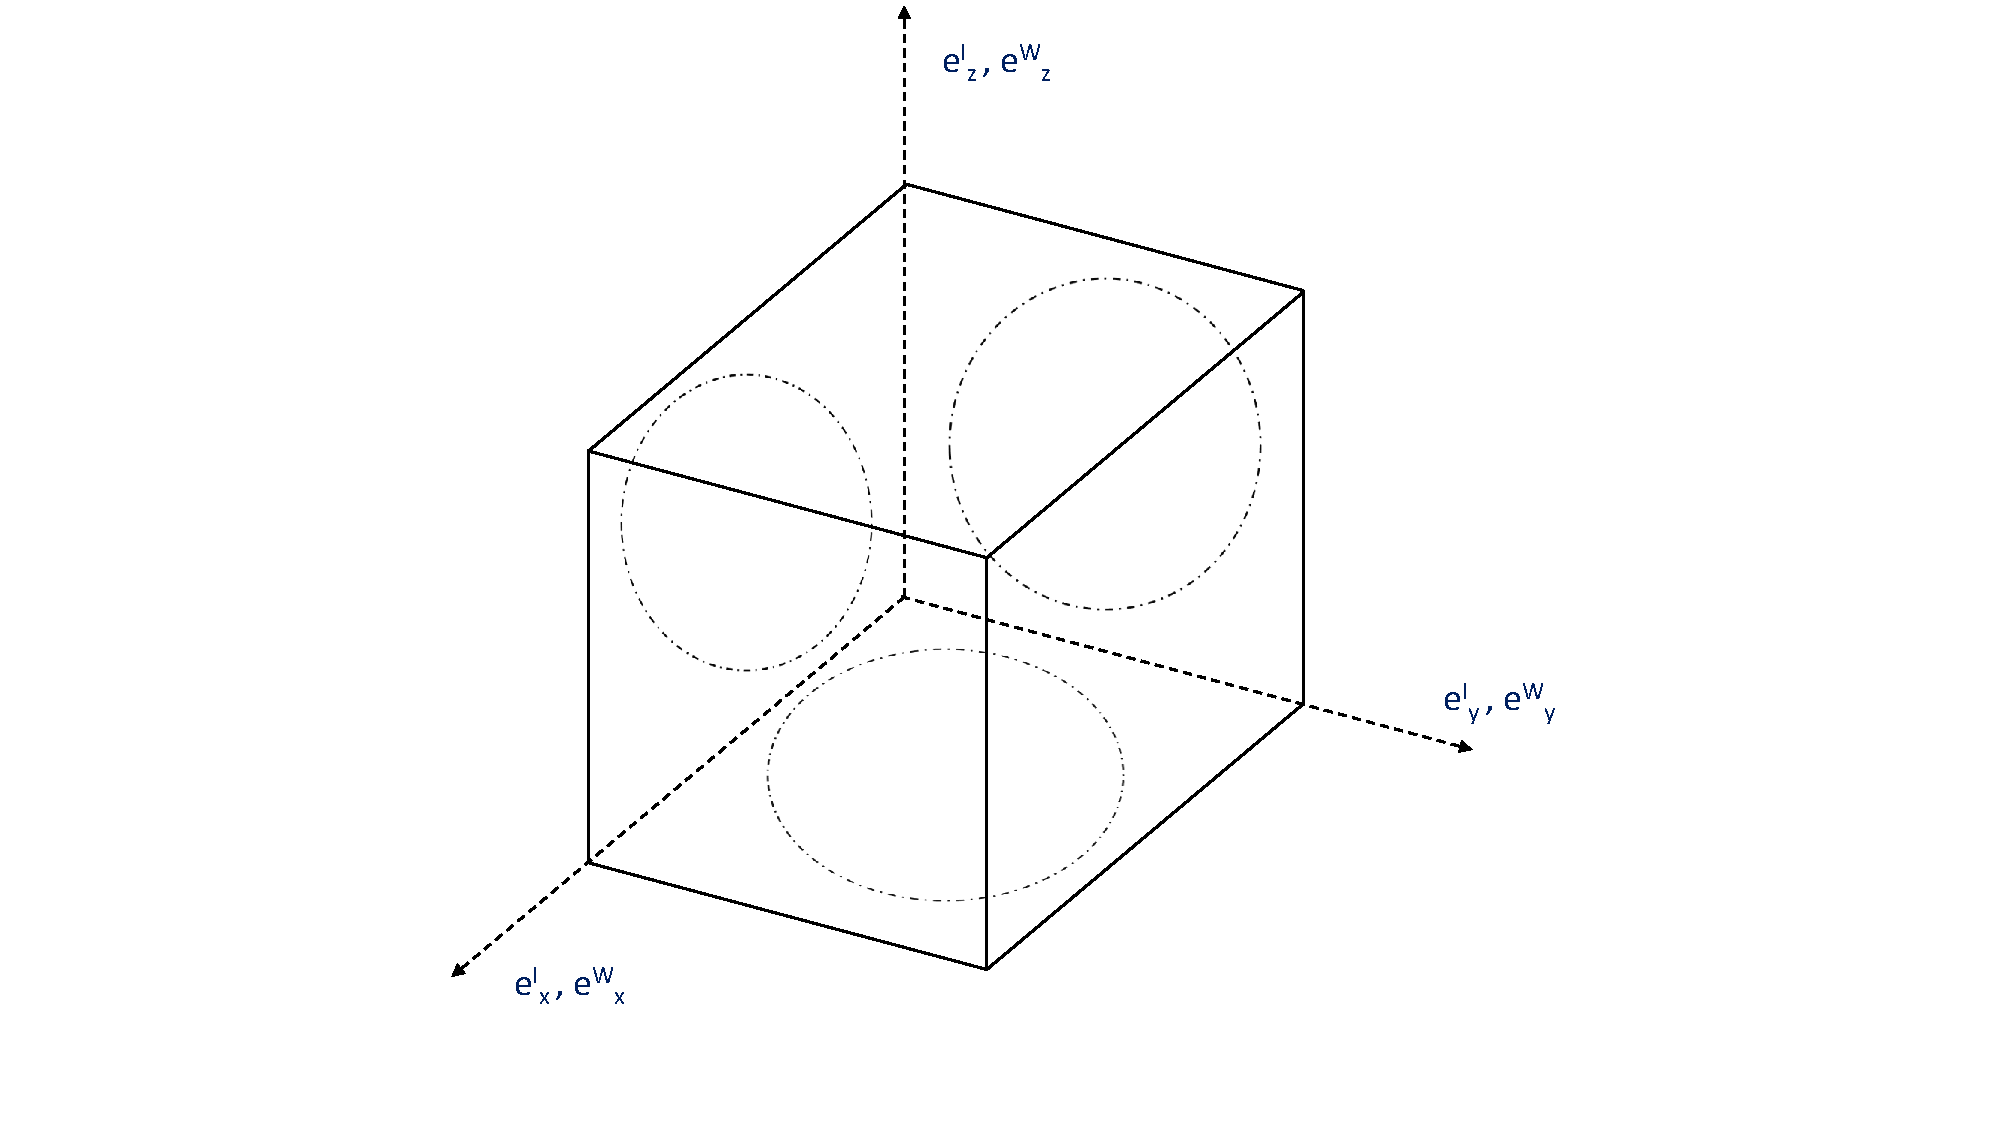
\includegraphics[width=\linewidth]{MechZeichnung3D}
\caption{Mechanischer Aufbau, Quelle: eigene Darstellung}
\end{figure}

Die aktuelle Position des Würfels kann somit eindeutig durch die Verschiebung des körperfesten Bezugssystems $\{W\}$ zu dem raumfesten Bezugssystem $\{I\}$ bestimmt werden. Um diese Rotation zu beschreiben werden die drei Euler-Winkel $\varphi_1$, $\varphi_2$ und $\varphi_3$ eingeführt. Die Drehreihenfolge und Drehachsen werden im folgenden beschrieben.

\begin{table}[h]
\centering
\begin{tabular}{|c|c|}
\hline
\textbf{Winkel} & \textbf{Beschreibung} \\ \hline
$\varphi_1$ & Drehung um $\inI e_z$ \\ \hline
$\varphi_2$ & Drehung um $\inW e_x$  \\ \hline
$\varphi_3$ & Drehung um $\inW e_z$ \\ \hline
\end{tabular}
\end{table}

Die erste Ableitung gewöhnliche Ableitung der Euler-Winkel entspricht den Winkelgeschwindigkeiten des Würfels um die oben genannten Achsen.

Mit Hilfe der Euler-Winkel können Drehmatrizen definiert werden um Koordinaten in dem raumfesten Bezugssystem $\{I\}$ in das körperfeste Bezugssystem $\{W\}$ zu projizieren. Hier zeigt sich wieder die Bedeutung der Reihenfolge der einzelnen Drehungen, da auch die Matrizenmultiplikation im Allgemeinen nicht kommutativ ist.

\begin{equation}
\inW{}\boldsymbol{r} = \inW{}\bS{D}_{\varphi_3} \cdot ( \inW{}\bS{D}_{\varphi_2} \cdot ( \inW{}\bS{D}_{\varphi_1} \cdot \inI{}\bS{r} )) = \inW{}\bS{D} \cdot \BinI{r}
\end{equation}

\begin{equation}
\inW{}\bS{D}_{\varphi_1} = \begin{pmatrix}
c_{\varphi_1} & -s_{\varphi_1} & 0 \\
s_{\varphi_1} & c_{\varphi_1} & 0 \\
0 & 0 & 1
\end{pmatrix}
\hspace{5pt}
\inW{}\bS{D}_{\varphi_2} = \begin{pmatrix}
1 & 0 & 0 \\
0 & c_{\varphi_2} & -s_{\varphi_2} \\
0 & s_{\varphi_2} & c_{\varphi_2}
\end{pmatrix}
\hspace{5pt}
\inW{}\bS{D}_{\varphi_3} = \begin{pmatrix}
c_{\varphi_3} & -s_{\varphi_3} & 0  \\
s_{\varphi_3} & c_{\varphi_3} & 0 \\
0 & 0 & 1
\end{pmatrix}
\end{equation}

\begin{equation}
\BinW{D} = \begin{pmatrix}
c_{\varphi_1}c{\varphi_3} - s_{\varphi_1}c_{\varphi_2}s_{\varphi_3} &
-c_{\varphi_1}s_{\varphi_3} - s_{\varphi_1}c_{\varphi_2}c_{\varphi_3} &
s_{\varphi_1}s_{\varphi_2} \\
s_{\varphi_1}c_{\varphi_3}+c_{\varphi_1}c_{\varphi_2}s_{\varphi_3} &
-s_{\varphi_1}s_{\varphi_3}+c_{\varphi_1}c_{\varphi_2}{\varphi_3} &
-c_{\varphi_1}s_{\varphi_2} \\
s_{\varphi_2}s_{\varphi_3} &
s_{\varphi_2}c_{\varphi_3} &
c_{\varphi_2}
\end{pmatrix}
\end{equation}

Die Projizierung einer Koordinate aus dem körperfesten in das raumfeste Bezugssystem erfolgt durch die transponierte der Matrix $\BinW{D}$.

\begin{equation}
\BinI{r} = \BinI{D} \cdot \BinI{r} = \BinW{D}^T \cdot  \BinI{r}
\end{equation} 

Die Bewegung der Schwungmassen relativ zu dem Würfelkörper wird von den drei Winkeln $\psi_1$, $\psi_2$ und $\psi_3$ beschrieben. Deren zeitliche Ableitungen stellen die Winkelgeschwindigkeiten der Schwungräder dar. 

\begin{equation}
\bS{\psi} = \begin{pmatrix}
{\psi}_1 \\
{\psi}_2  \\
{\psi}_3 
\end{pmatrix}
\hspace{35pt}
\bS{\dot{\psi}} = \begin{pmatrix}
\dot{\psi}_1 \\
\dot{\psi}_2  \\
\dot{\psi}_3 
\end{pmatrix}
\end{equation}

Die Euler-Winkel $\bS{\varphi}$ und die Ausfallwinkel der Schwungmassen $\bS{\psi}$ werden als generalisierte Koordinaten verwendet.

\begin{equation}
\bS{q} = \begin{pmatrix}
q_1 \\ q_2 \\ q_3 \\ q_4 \\ q_5 \\ q_6
\end{pmatrix} =
\begin{pmatrix}
\varphi_1 \\ \varphi_2 \\ \varphi_3 \\ \psi_1 \\ \psi_2 \\ \psi_3
\end{pmatrix}
\end{equation}

\subsubsection{Potential des Systems}
Um die Lagrange-Funktion $L$ des Systems zu bestimmen muss einerseits die kinetische Energie $T$ und die potentielle Energie $V$ ermittelt werden. Das Potential des Würfels wird durch die aktuelle Lage seines Schwerpunktes $\bS{r}$ bestimmt, hierbei ist lediglich die z-Komponente des raumfesten Bezugssystem von Bedeutung.

\begin{equation}
V = m_G \cdot g \cdot \inI z_{cog}
\end{equation}

Die Position des Schwerpunktes im körperfesten Bezugssystem ist fix. Durch die Projektion dieses Vektors $\BinW{r}_{cog}$ in das raumfeste Bezugssystem $\{I\}$ wird die Abhängigkeit von der aktuellen Verschiebung berücksichtigt.

\begin{equation}
\BinI{r}_C = \BinI{D} \cdot \BinW{r}_{C} = \BinI{D} \cdot \begin{pmatrix}
\inW x_C \\ \inW y_C \\ \inW z_C
\end{pmatrix}
\end{equation}

Folglich ergibt sich der folgende Zusammenhang für das Potential $V$ und die aktuelle Ausrichtung des Würfels.

\begin{equation}
V = m_G \cdot g \cdot \inI z_{cog} = m_G \cdot g \cdot (s_{\varphi_2}s_{\varphi3} \cdot \inW x_C + s_{\varphi_2}c_{\varphi_3} \cdot \inW y_C  + c_{\varphi_2} \cdot \inW z_C)
\end{equation}

\subsubsection{Kinetische Energie des Systems}
Die kinetische Energie setzt sich aus der Winkelgeschwindigkeit des Würfels $\bS{\omega}_K$ und der Geschwindigkeiten der drei Schwungmassen $\bS{\omega}_R$ zusammen. Hierbei ist zu beachten, dass die Winkelgeschwindigkeiten in verschiedenen Bezugssystemen darstellbar sind und die kinetische Energie von der Darstellungsform unabhängig ist. Um dies zu gewährleisten müssen allerdings auch die Trägheitstensoren in das jeweilige Bezugssystem projiziert werden.

\begin{equation}
\BinW{\omega}_K = \begin{pmatrix}
\inW \omega_x \\
\inW \omega_y \\
\inW \omega_z
\end{pmatrix}
\hspace{35pt}
\BinW{\omega}_R = \dot{\bS{\psi}}
\end{equation}

\begin{equation}
T = \frac{1}{2} \BinW{\omega}^T_K \cdot (\BinW{\Theta}_G - \BinW{\Theta}_R) \cdot \BinW{\omega}_K + \frac{1}{2} (\BinW{\omega}_K + \BinW{\omega}_R)^T \cdot \BinW{\Theta}_R \cdot (\BinW{\omega}_K + \BinW{\omega}_R)
\end{equation}

Um das die kinetische Energie $T$ mit Hilfe der generalisierten Koordinaten darzustellen muss die Winkelgeschwindigkeit $\BinW{\omega}_W$ als die erste Ableitung der Euler-Winkel $\bS{\varphi}$ darstellen.
Um die Projektion der Euler-Geschwindigkeiten $\dot{\bS{\varphi}}$ zu veranschaulichen kann die Rotationsgeschwindigkeit des Würfels $\BinW{\omega}_W$ als Summe der Euler-Komponenten dargestellt werden.

\begin{equation}
\BinW{\omega}_W = \BinW{\dot{\varphi}_1} + \BinW{\dot{\varphi}_2} + \BinW{\dot{\varphi}_3}
\end{equation}

Um die Euler-Geschwindigkeit in dem körperfesten Bezugssystem darzustellen werden Rotationsachsen um die entsprechenden Euler-Winkel rotiert. Die Winkelgeschwindigkeit $\dot{\varphi}_3$ ist ist gleich der Rotation um die körperfeste $\inW e_z$ und muss somit nicht über eine Drehmatrix projiziert werden. 

\begin{equation}
\BinW{\dot{\varphi}}_3 =  =
\begin{pmatrix}
0 \\ 0 \\ \inW{\omega}_z
\end{pmatrix} 
\end{equation}

Die Winkelgeschwindigkeit $\dot{\varphi}_2$ entsprecht der Rotation um die körperfeste Achse $\inW e_x$ vor der Rotation um den Winkel $\varphi_3$. Somit muss mit Hilfe der  Matrix $\BinW{D}_{\varphi_3}$ der Geschwindigkeitsvektor in das endgültige körperfeste Bezugssystem projiziert werden.

\begin{equation}
\BinW{\dot{\varphi}}_2 = \BinW{D}_{\varphi_3} \cdot
\begin{pmatrix}
\dot{\varphi}_2 \\ 0 \\ 0
\end{pmatrix} = 
\begin{pmatrix}
\dot{\varphi}_2 \cdot c_{\varphi_3} \\
-\dot{\varphi}_2 \cdot s_{\varphi_3} \\
0
\end{pmatrix}
\end{equation}

Die dritte Komponente ist die Winkelgeschwindigkeit $\dot{\varphi}_1$, welche der Rotation um die raumfeste Achse $\inI e_z$ entspricht. Folglich muss zu einer Projektion in das körperfeste Bezugsystem der Geschwindigkeitsvektor mit den Matrizen $\BinW{D}_{\varphi_3}$ und $\BinW{D}_{\varphi_2}$ multipliziert werden. 

\begin{equation}
\BinW{\omega}_W = \BinW{\dot{\varphi}_1} + \BinW{\dot{\varphi}_2} + \BinW{\dot{\varphi}_3} = 
(\BinW{D}_{\varphi_2} (
\BinW{D}_{\varphi_3} \cdot \begin{pmatrix}
\dot{\varphi}_1 \\ 0 \\ 0
\end{pmatrix} ) )
=
\begin{pmatrix}
\dot{\varphi}_1 \cdot s_{\varphi_2} \cdot s_{\varphi_3} \\
\dot{\varphi}_1 \cdot s_{\varphi_2} \cdot c_{\varphi_3} \\
\dot{\varphi}_1 \cdot c_{\varphi_2}
\end{pmatrix}
\end{equation}

Die gesamte Winkelgeschwindigkeit des Würfels $\BinW{\omega}_K$ ergibt sich wie bereits beschrieben aus der Summe der einzelnen Komponenten.

\begin{equation}
\BinW{\dot{\varphi}} = 
\begin{pmatrix}
\dot{\varphi}_1 \cdot s_{\varphi_2} \cdot s_{\varphi_3} + \dot{\varphi}_2 \dot c_{\varphi_3} \\
\dot{\varphi}_1 \cdot s_{\varphi_2} \cdot c_{\varphi_3} - \dot{\varphi}_2 \cdot s_{\varphi_3} \\
\dot{\varphi}_1 \cdot c_{\varphi_2} + \dot{\varphi}_3
\end{pmatrix}
\end{equation}



\subsubsection{Generalisierte Kraftkomponenten}
In der Untersuchung des 1D-Modelles wurde bereits gezeigt, dass der Würfel ein nicht konservatives System ist, da einerseits über die Motoren mechanische Energie zugeführt wird und andererseits durch Reibung mechanische Energie verloren geht. Deshalb müssen die generalisierten Kraftkomponenten bestimmt werden um mit Hilfe des d'Alembert'schen Prinzip die Bewegungsgleichungen zu ermitteln.
\newline

Wie bereits angesprochen erzeugen die Motoren Momente, welche die Schwungmassen antreiben. Gleichermaßen entsteht in den Lagern der Räder ein Reibmoment welches als linear abhängig von der Winkelgeschwindigkeit modelliert wird. Somit ergibt sich das folgende Moment.

\begin{equation}
\BinW{M}_M = \BinW{T}_M - \bS{C}_{\psi} \cdot \BinW{\dot {\psi}} \hspace{35pt} \bS{C}_{\psi} = \begin{pmatrix}
C_{\psi_1} & 0 & 0 \\
0 & C_{\psi_2} & 0 \\
0 & 0 & C_{\psi_3}
\end{pmatrix}
\end{equation}

Die Komponenten dieses Momentvektors sind gleichermaßen die generalisierten Kraftkomponenten der Koordinaten $\psi_1$, $\psi_2$ und $\psi_3$.

\begin{equation}
Q_{\psi_1} = Q_4 = T_{M1} - C_{\psi_1} \cdot \dot{\psi}_1
\end{equation}
\begin{equation}
Q_{\psi_2} = Q_5 = T_{M2} - C_{\psi_2} \cdot \dot{\psi}_2
\end{equation}
\begin{equation}
Q_{\psi_3} = Q_6 = T_{M3} - C_{\psi_3} \cdot \dot{\psi}_3
\end{equation}

Die Kraftkomponenten, welche den generalisierten Koordinaten $\varphi_1$, $\varphi_2$ und $\varphi_3$ zugeordnet sind lassen sich aus dem Potential $V$ herleiten.

\begin{equation}
Q_{\varphi_1} = \frac{\partial V}{\partial \varphi_1} = 0
\end{equation}

\begin{equation}
Q_{\varphi_2} = \frac{\partial V}{\partial \varphi_2} = m_G \cdot g \cdot (c_{\varphi_2} s_{\varphi_3} \cdot \inW{y}_C + c_{\varphi_2}c_{\varphi_3} \cdot \inW{y}_C - s_{\varphi_2} \cdot \inW{z}_C)
\end{equation}

\begin{equation}
Q_{\varphi_3} = \frac{\partial V}{\partial \varphi_3} = m_G \cdot g \cdot (s_{\varphi_2} c_{\varphi_3} \cdot \inW{x}_C - s_{\varphi_2} c_{\varphi_3} \cdot \inW{y}_C)
\end{equation}



\newpage
\begin{thebibliography}{\hspace{0.5cm}}
	\bibitem{Cubli1D} Mohanarjah Gajamohan, Michael merz, Igor Thommen, Raffaello D'Andrea: The Cubli: A Cube that can Jump Up and Balance
	\bibitem{Cubli3D_LQR} Mohanarajah Gajamohan, Michael Muehlbach, Tobias Widmer, Raffaello D'Andrea: The Cubli: A Reaction Wheel Based 3D Inverted Pendulum
	\bibitem{Cubli3D_Nonlinear} Michael Muehlbach, Gajamohan Mohanarajah, Raffaello D'Andrea: Nonlinear Analysis and Control of a Reaction Wheel-based 3D Inverted Pendulum
	\bibitem{TheoPhysik1} Wolfgang Nolting: Grundkurs Theoretische Physik 1 - Klassische Mechanik
	\bibitem{TheoPhysik2} Wolfgang Nolting: Grundkurs Theoretische Physik 2 - Analytische Mechanik
	\bibitem{Kane} Thomas R. Kane: Dynamics - Theory and Applications
	\bibitem{PraxisDerDigSigVer} Fernando Puente Le\'on, Sebastian Bauer: Praxis der digitalen Signalverarbeitung
	\bibitem{SimTechLinearUndNichtlinSysteme} Josef Hoffmann, Franz Quint : Simulation technischer linearer und nichtlinearer Systeme mit MATLAB/Simulink
	\bibitem{SystemTheoStochPro} Herbert Schlitt: Systemtheorie für stochastische Prozesse
	\bibitem{SigVer_AnaDigSig} Marin Meyer: Signalverarbeitung - Analoge und digitale Signale, Systeme und Filter
	\bibitem{SuS} Ottmar Beucher: Signale und Systeme - Theorie, Simulation und Anwendung
	\bibitem{RT1} Heinz Unbehauen: Regelungstechnik 1 - Klassische Verfahren zur Analyse und Synthese linearer kontinuierlicher Regelsysteme
	\bibitem{RT2} Heinz Unbehauen: Regelungstechnik 2 - Zustandsregelungen, digitale und nichtlineare Regelsysteme
	\bibitem{lqrnotes} Joao P. Hespanha: Lecture notes on LQR/LQG controller design
	\bibitem{ML_Mitchell} Tom M. Mitchell: Machine Learning
	\bibitem{ML_Bishop} Christopher Bishop: Pattern Recognition and Machine Learning
	\bibitem{Wie_FW} Joachim Wietzke, Manh Tien Tran: Automotive Embedded Systeme: Effizientes Framework - Vom Design zur Implementierung
	\bibitem{Wie_ET} Joachim Wietzke: Embedded Technologies: Vom Treiber bis zur Grafik-Anbindung
	\bibitem{EBBB} Derek Molloy: Exploring BeagleBone: Tools and Techniques for Building with Embedded Linux
\end{thebibliography}

\section{Anhang}

\begin{landscape}

	\begin{figure} 
	\begin{center}
	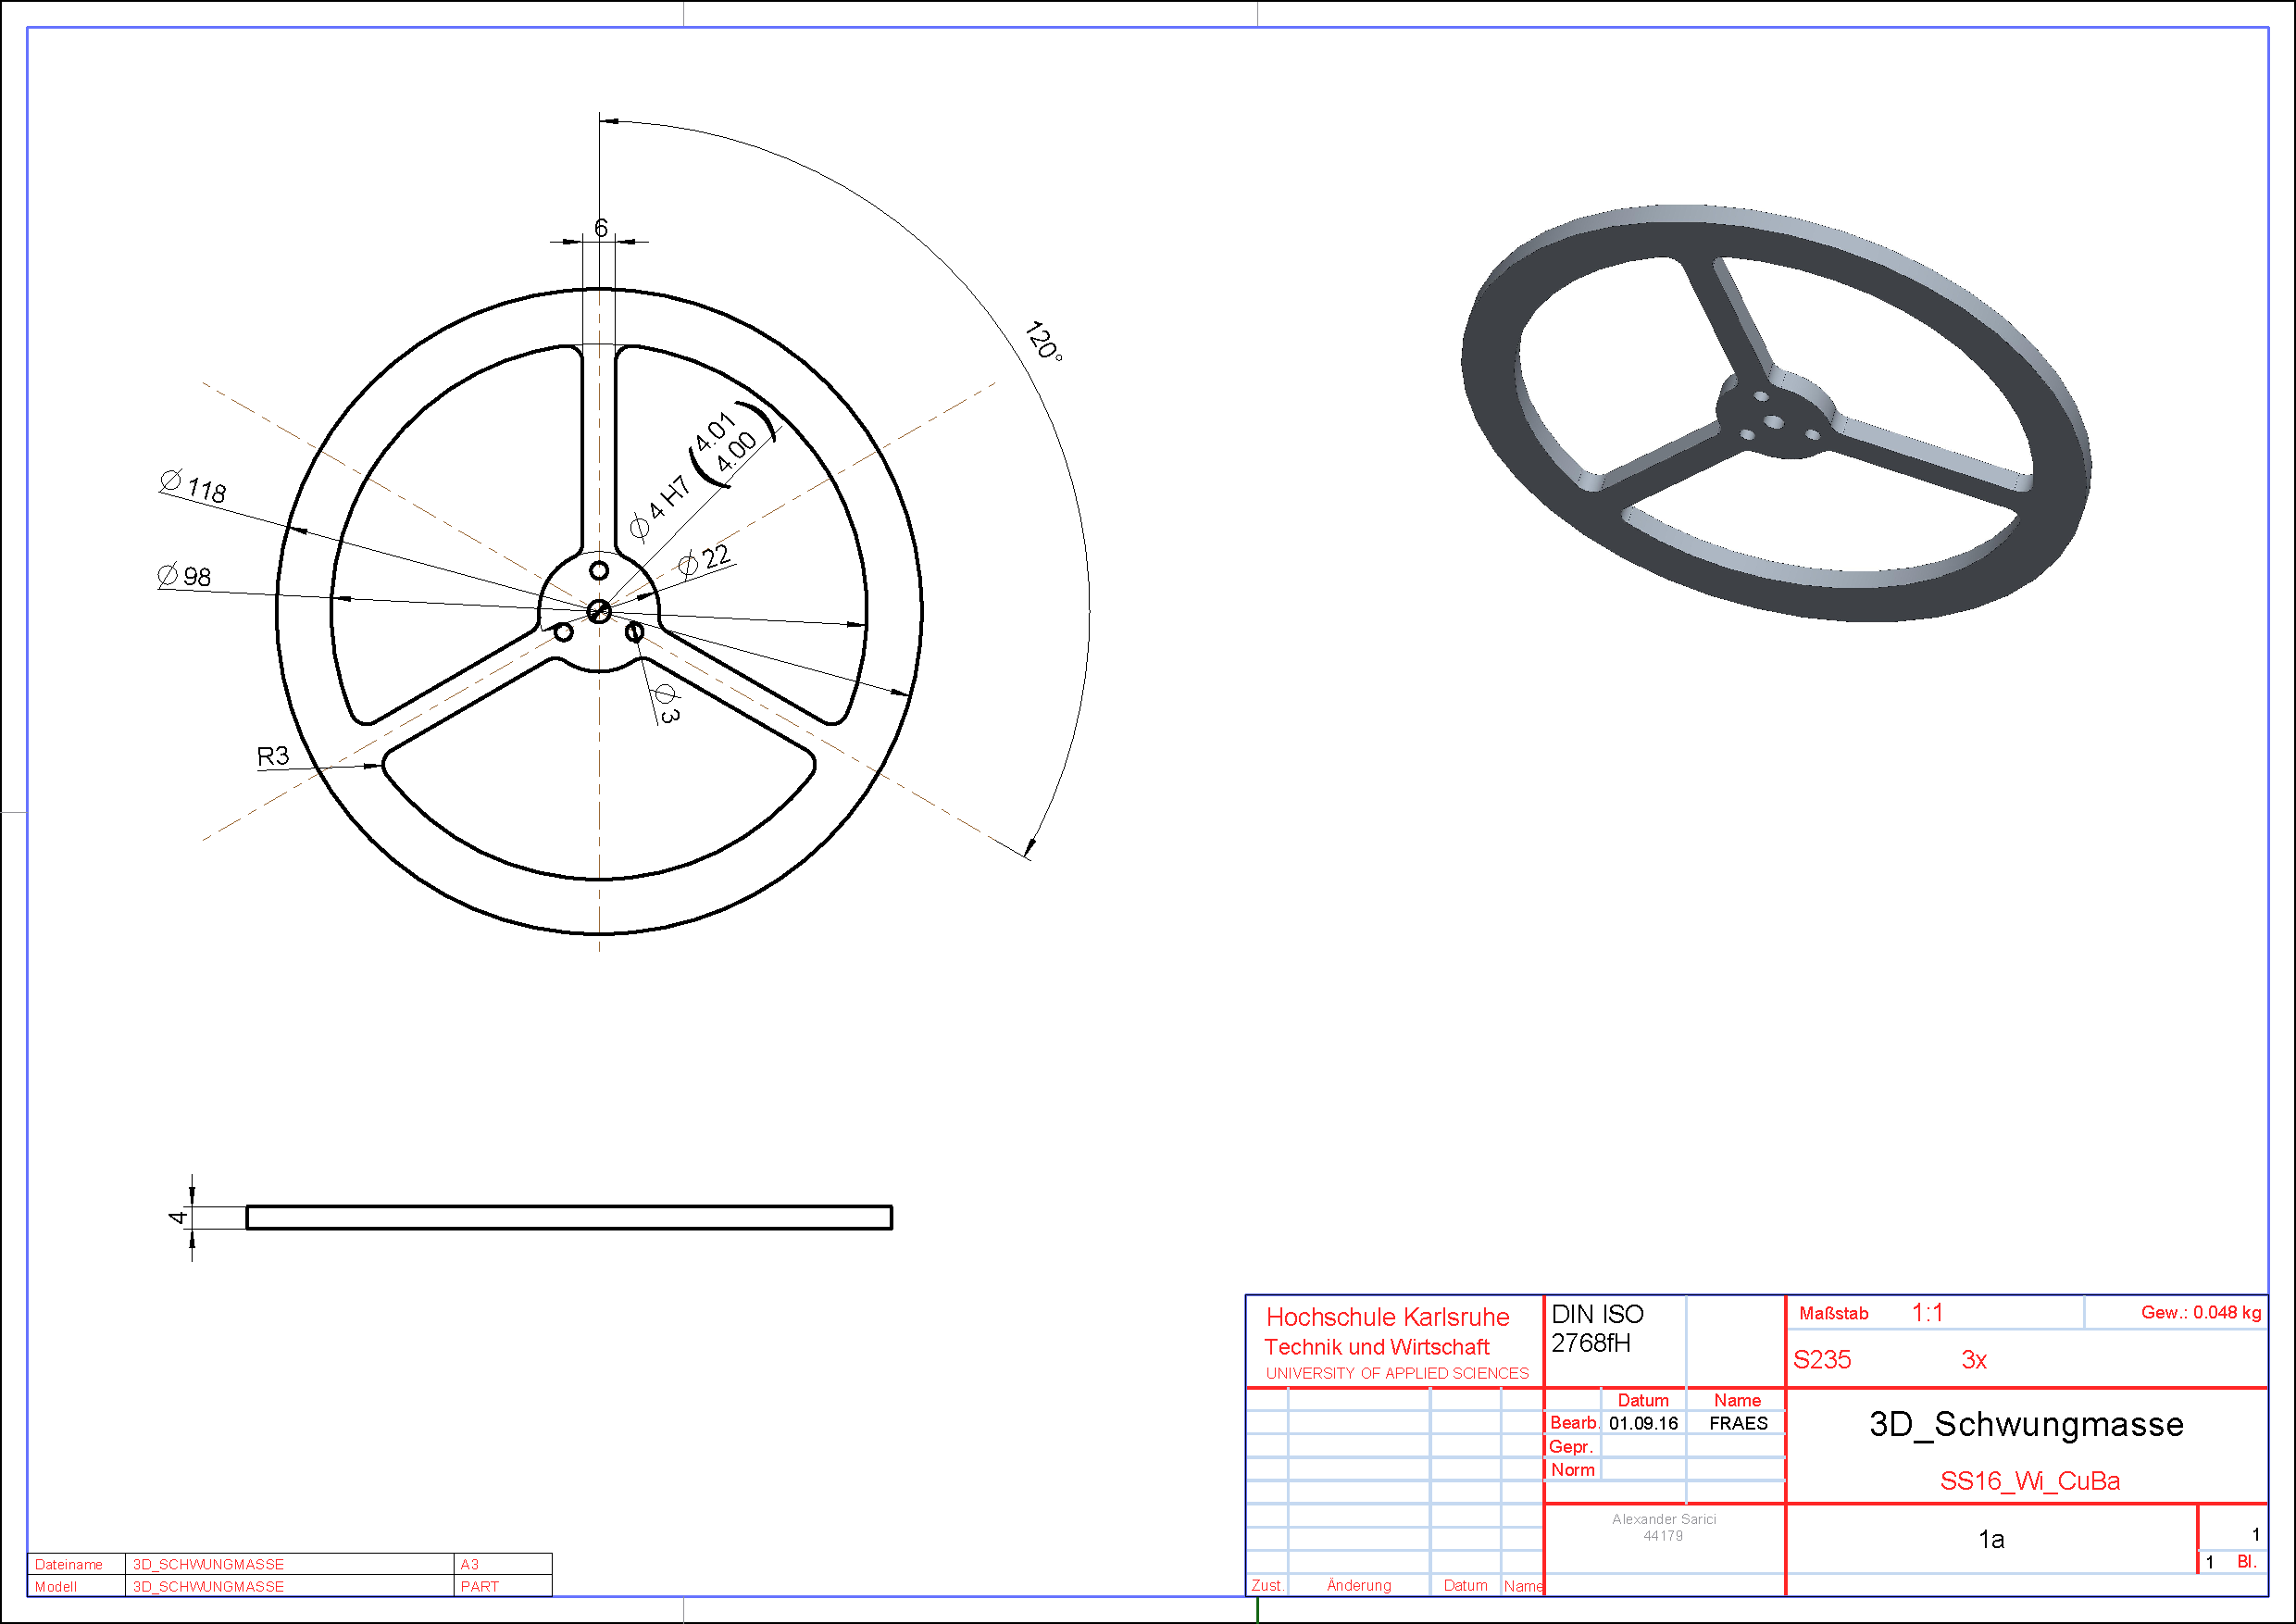
\includegraphics[width=1.5\textwidth]{img/3d_schwungmasse.pdf}
	\end{center}
	\caption{Technische Zeichnung Schwungmasse, Quelle: eigene Darstellung}
	\end{figure} 
	
	\begin{figure} 
	\begin{center}
	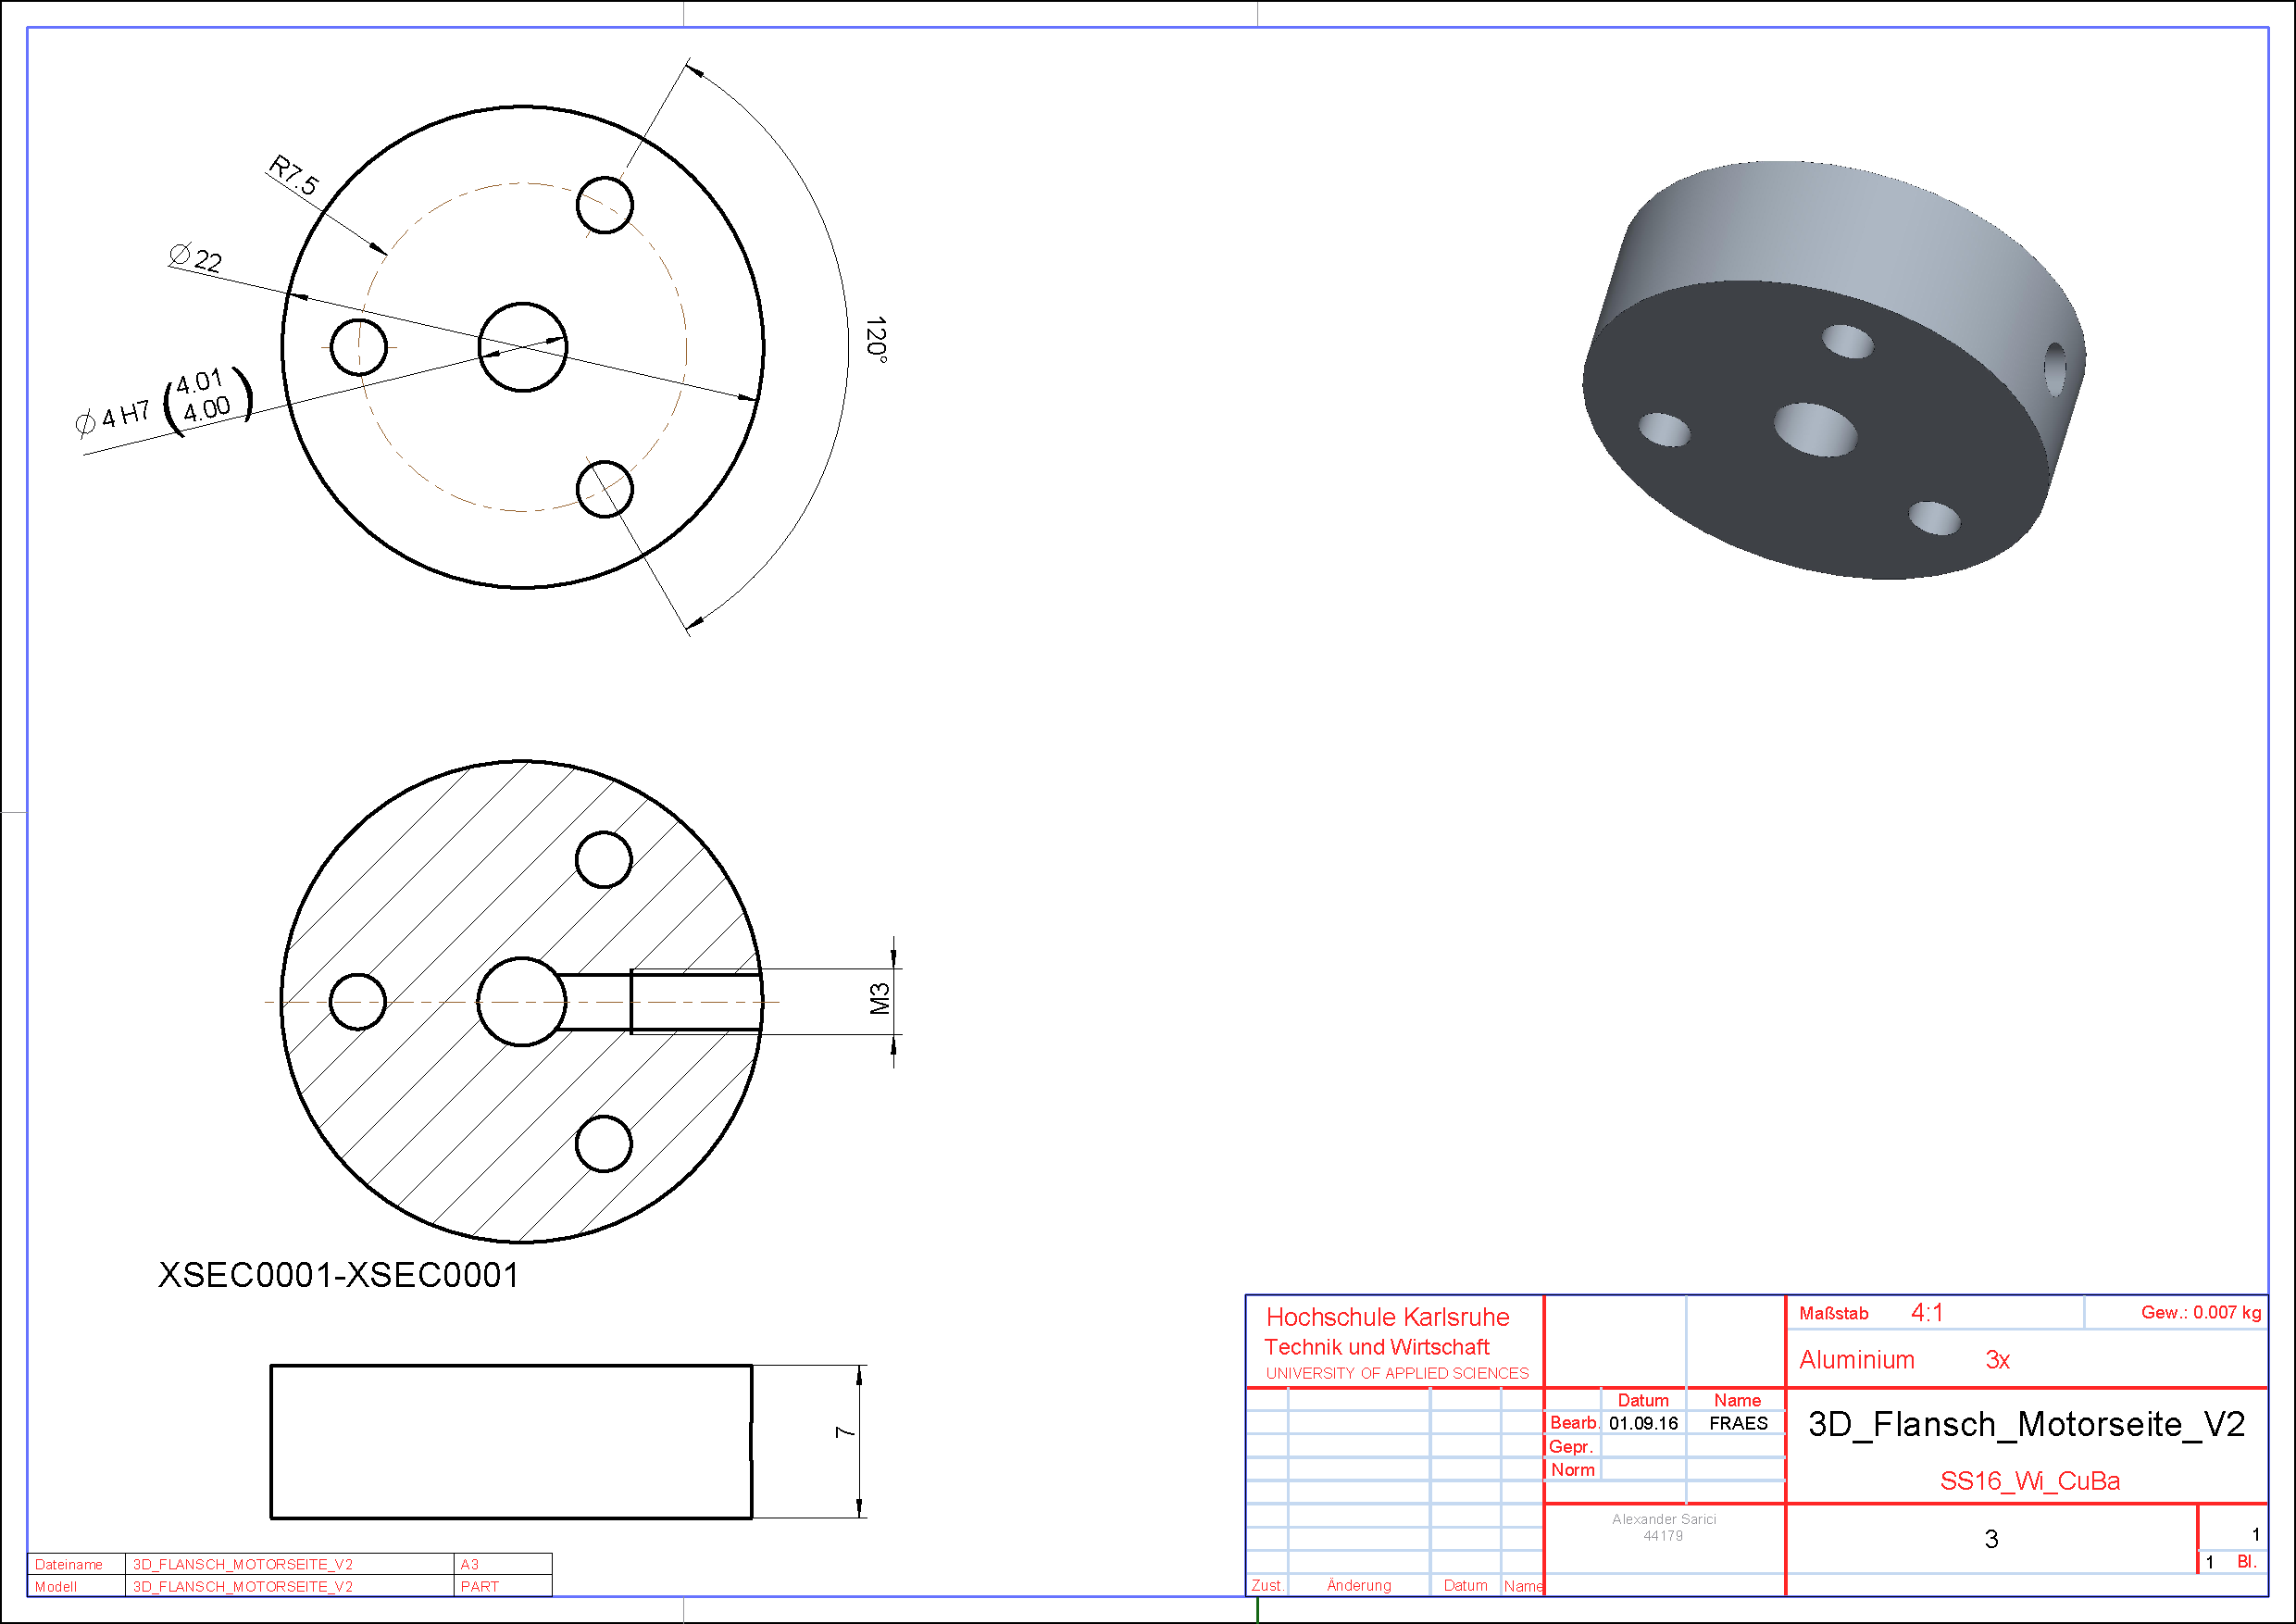
\includegraphics[width=1.5\textwidth]{img/3d_flansch_motorseite_v2.pdf}
	\end{center}
	\caption{Technische Zeichnung Flansch Motorseite, Quelle: eigene Darstellung}
	\end{figure} 
		
	\begin{figure} 
	\begin{center}
	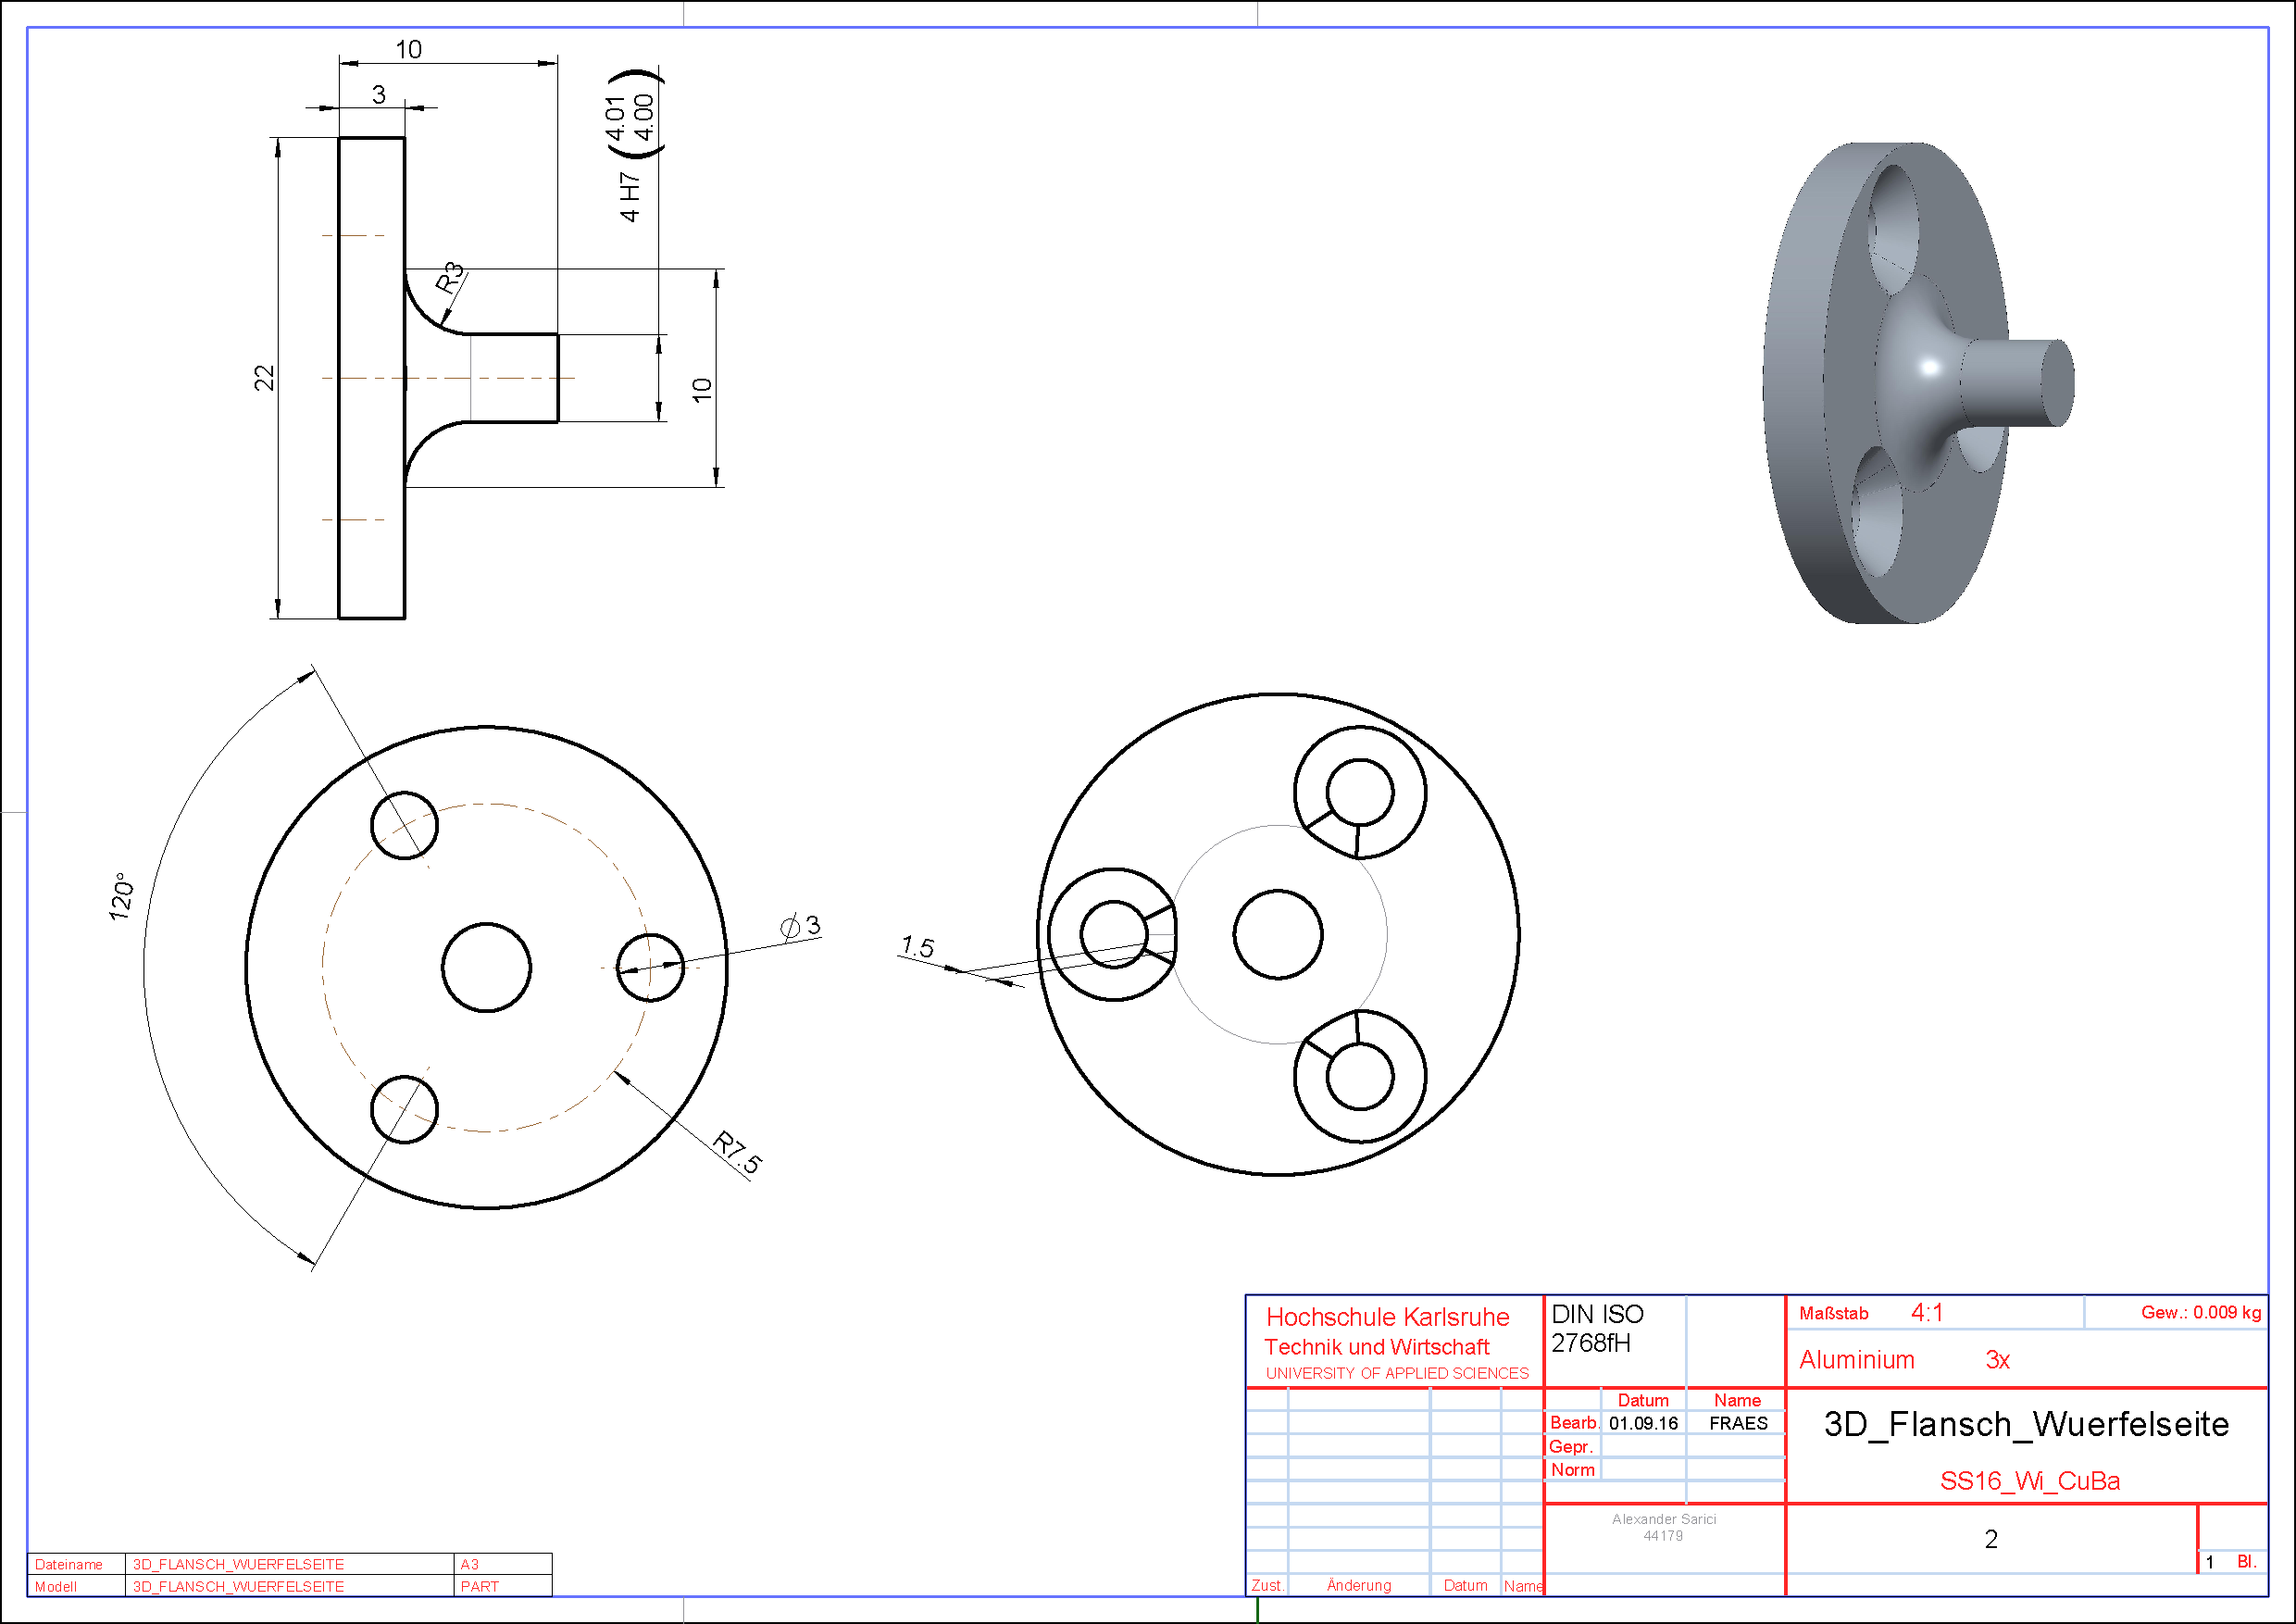
\includegraphics[width=1.5\textwidth]{img/3d_flansch_wuerfelseite.pdf}
	\end{center}
	\caption{Technische Zeichnung Flansch Würfelseite, Quelle: eigene Darstellung}
	\end{figure}
	
	\begin{figure} 
	\begin{center}
	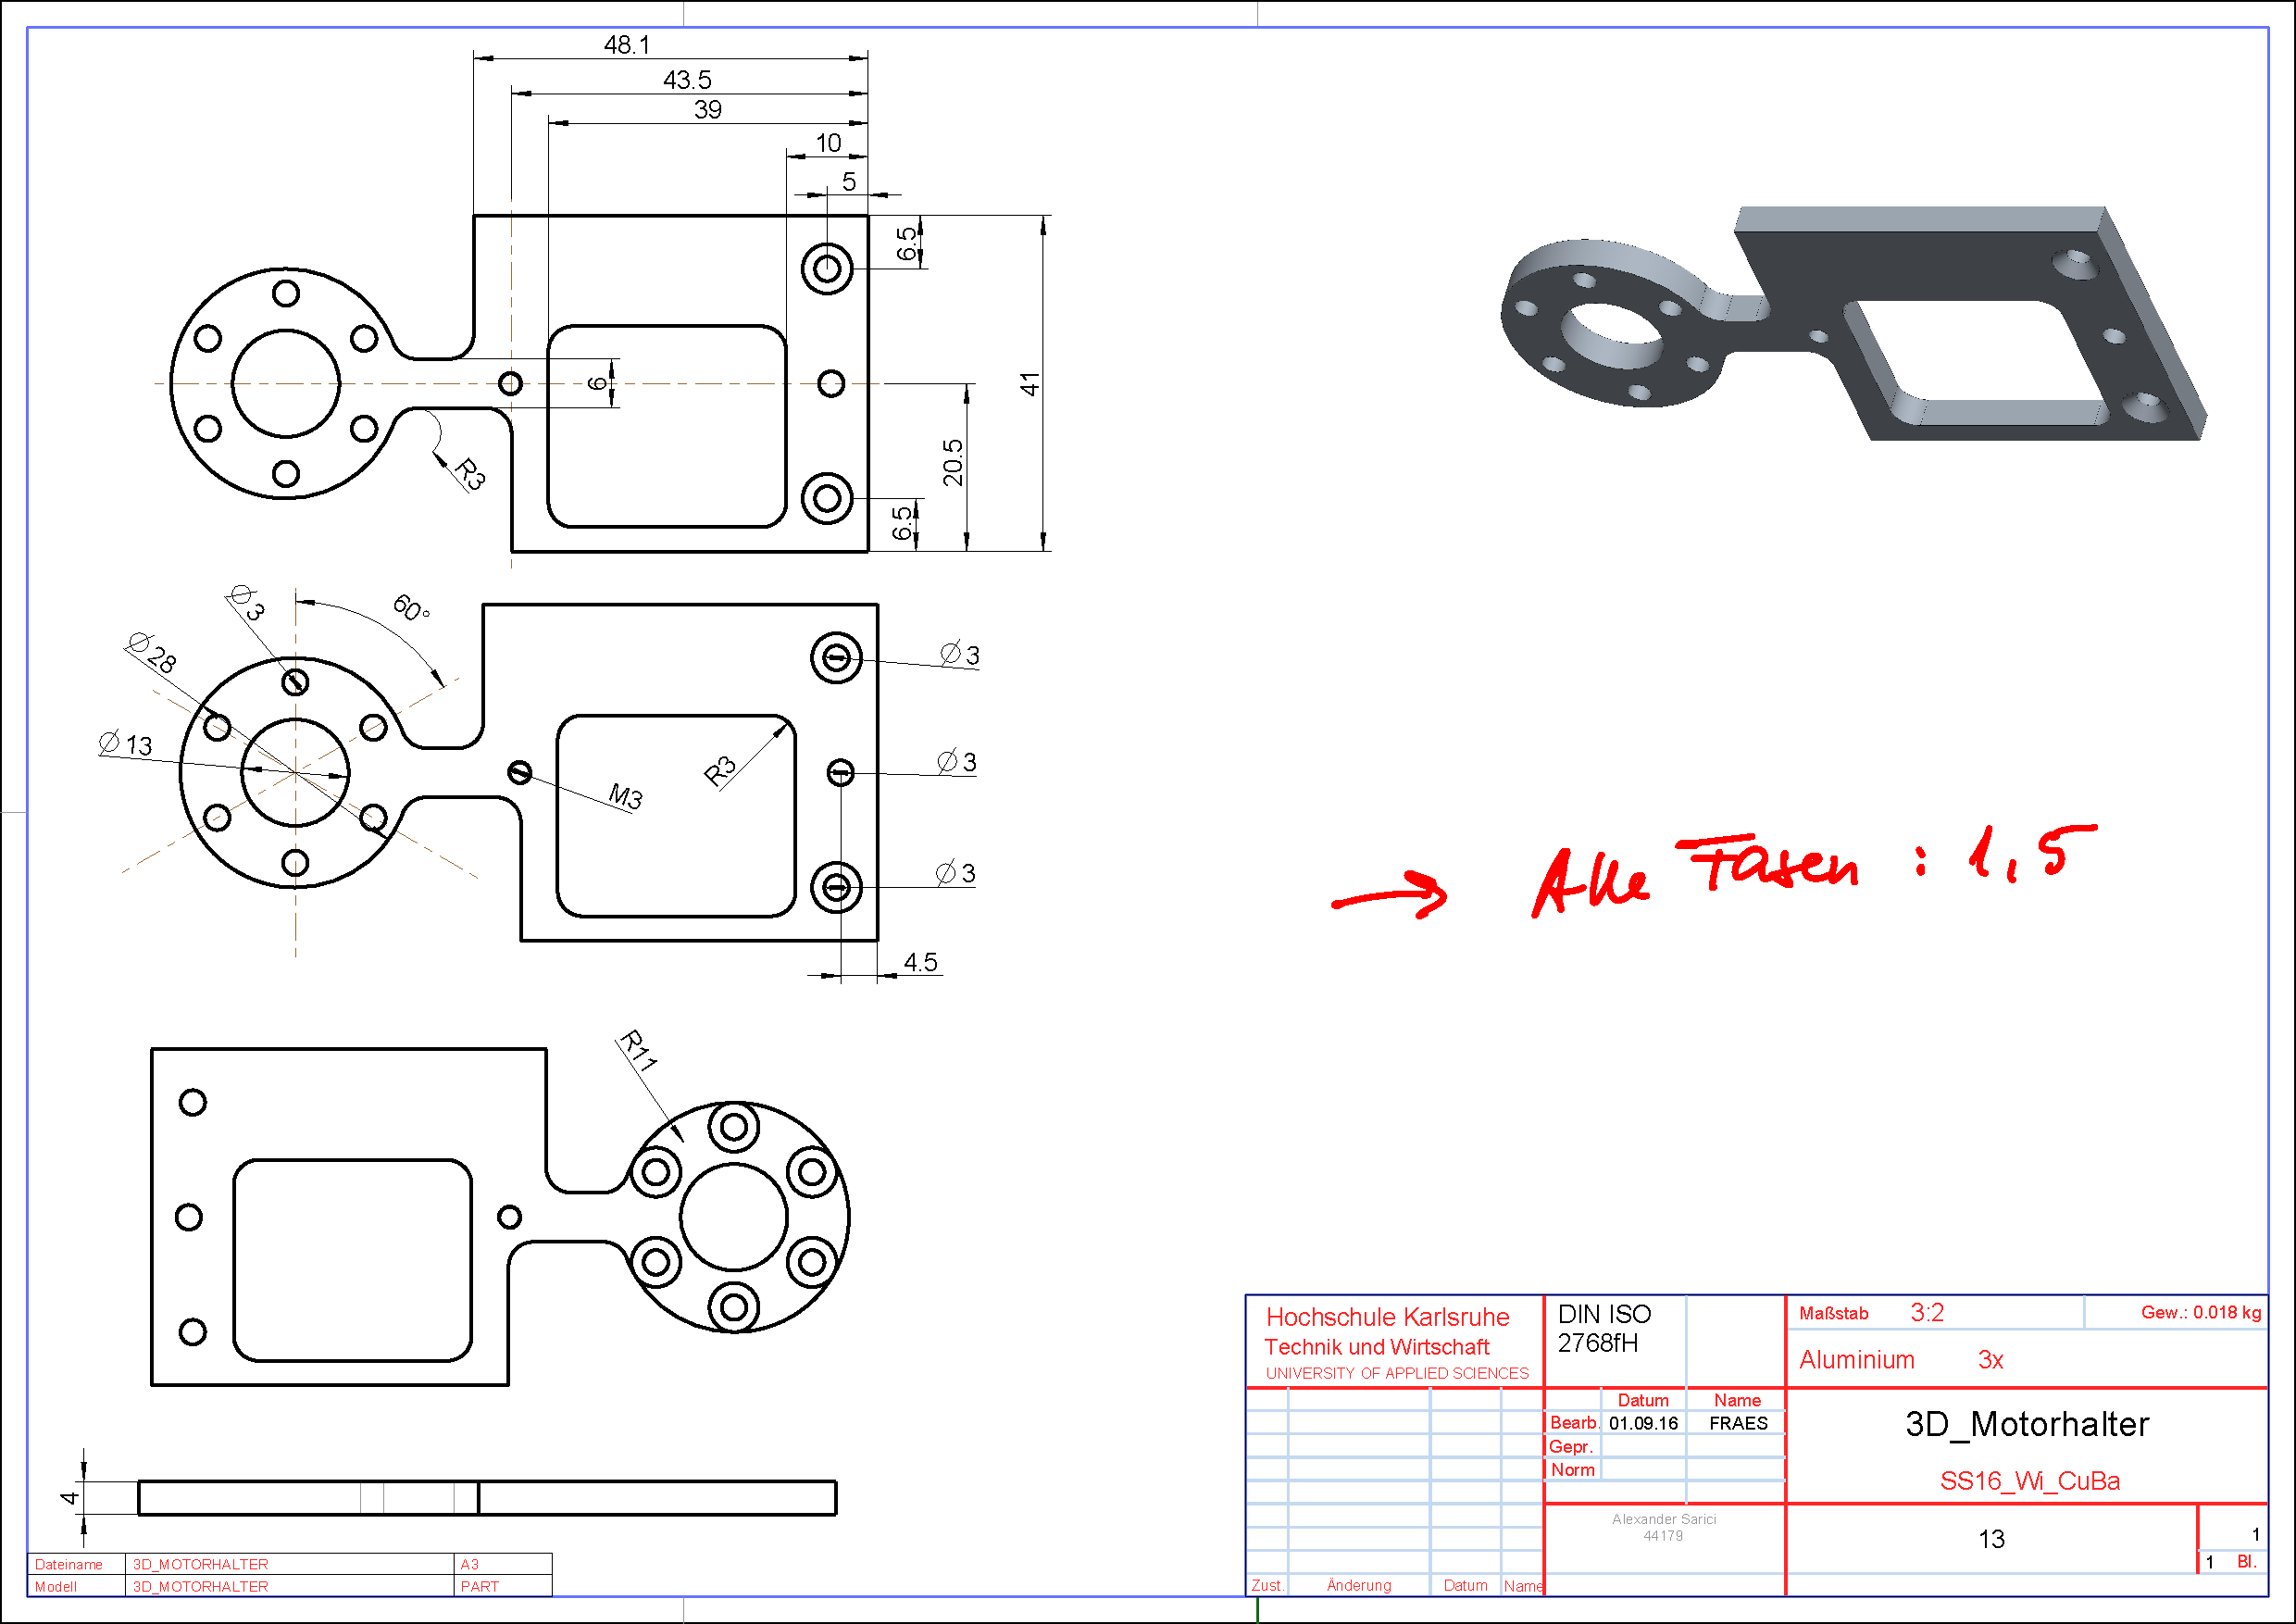
\includegraphics[width=1.5\textwidth]{img/3d_motorhalter.pdf}
	\end{center}
	\caption{Technische Zeichnung Motorhalter, Quelle: eigene Darstellung}
	\end{figure} 
	
	\begin{figure} 
	\begin{center}
	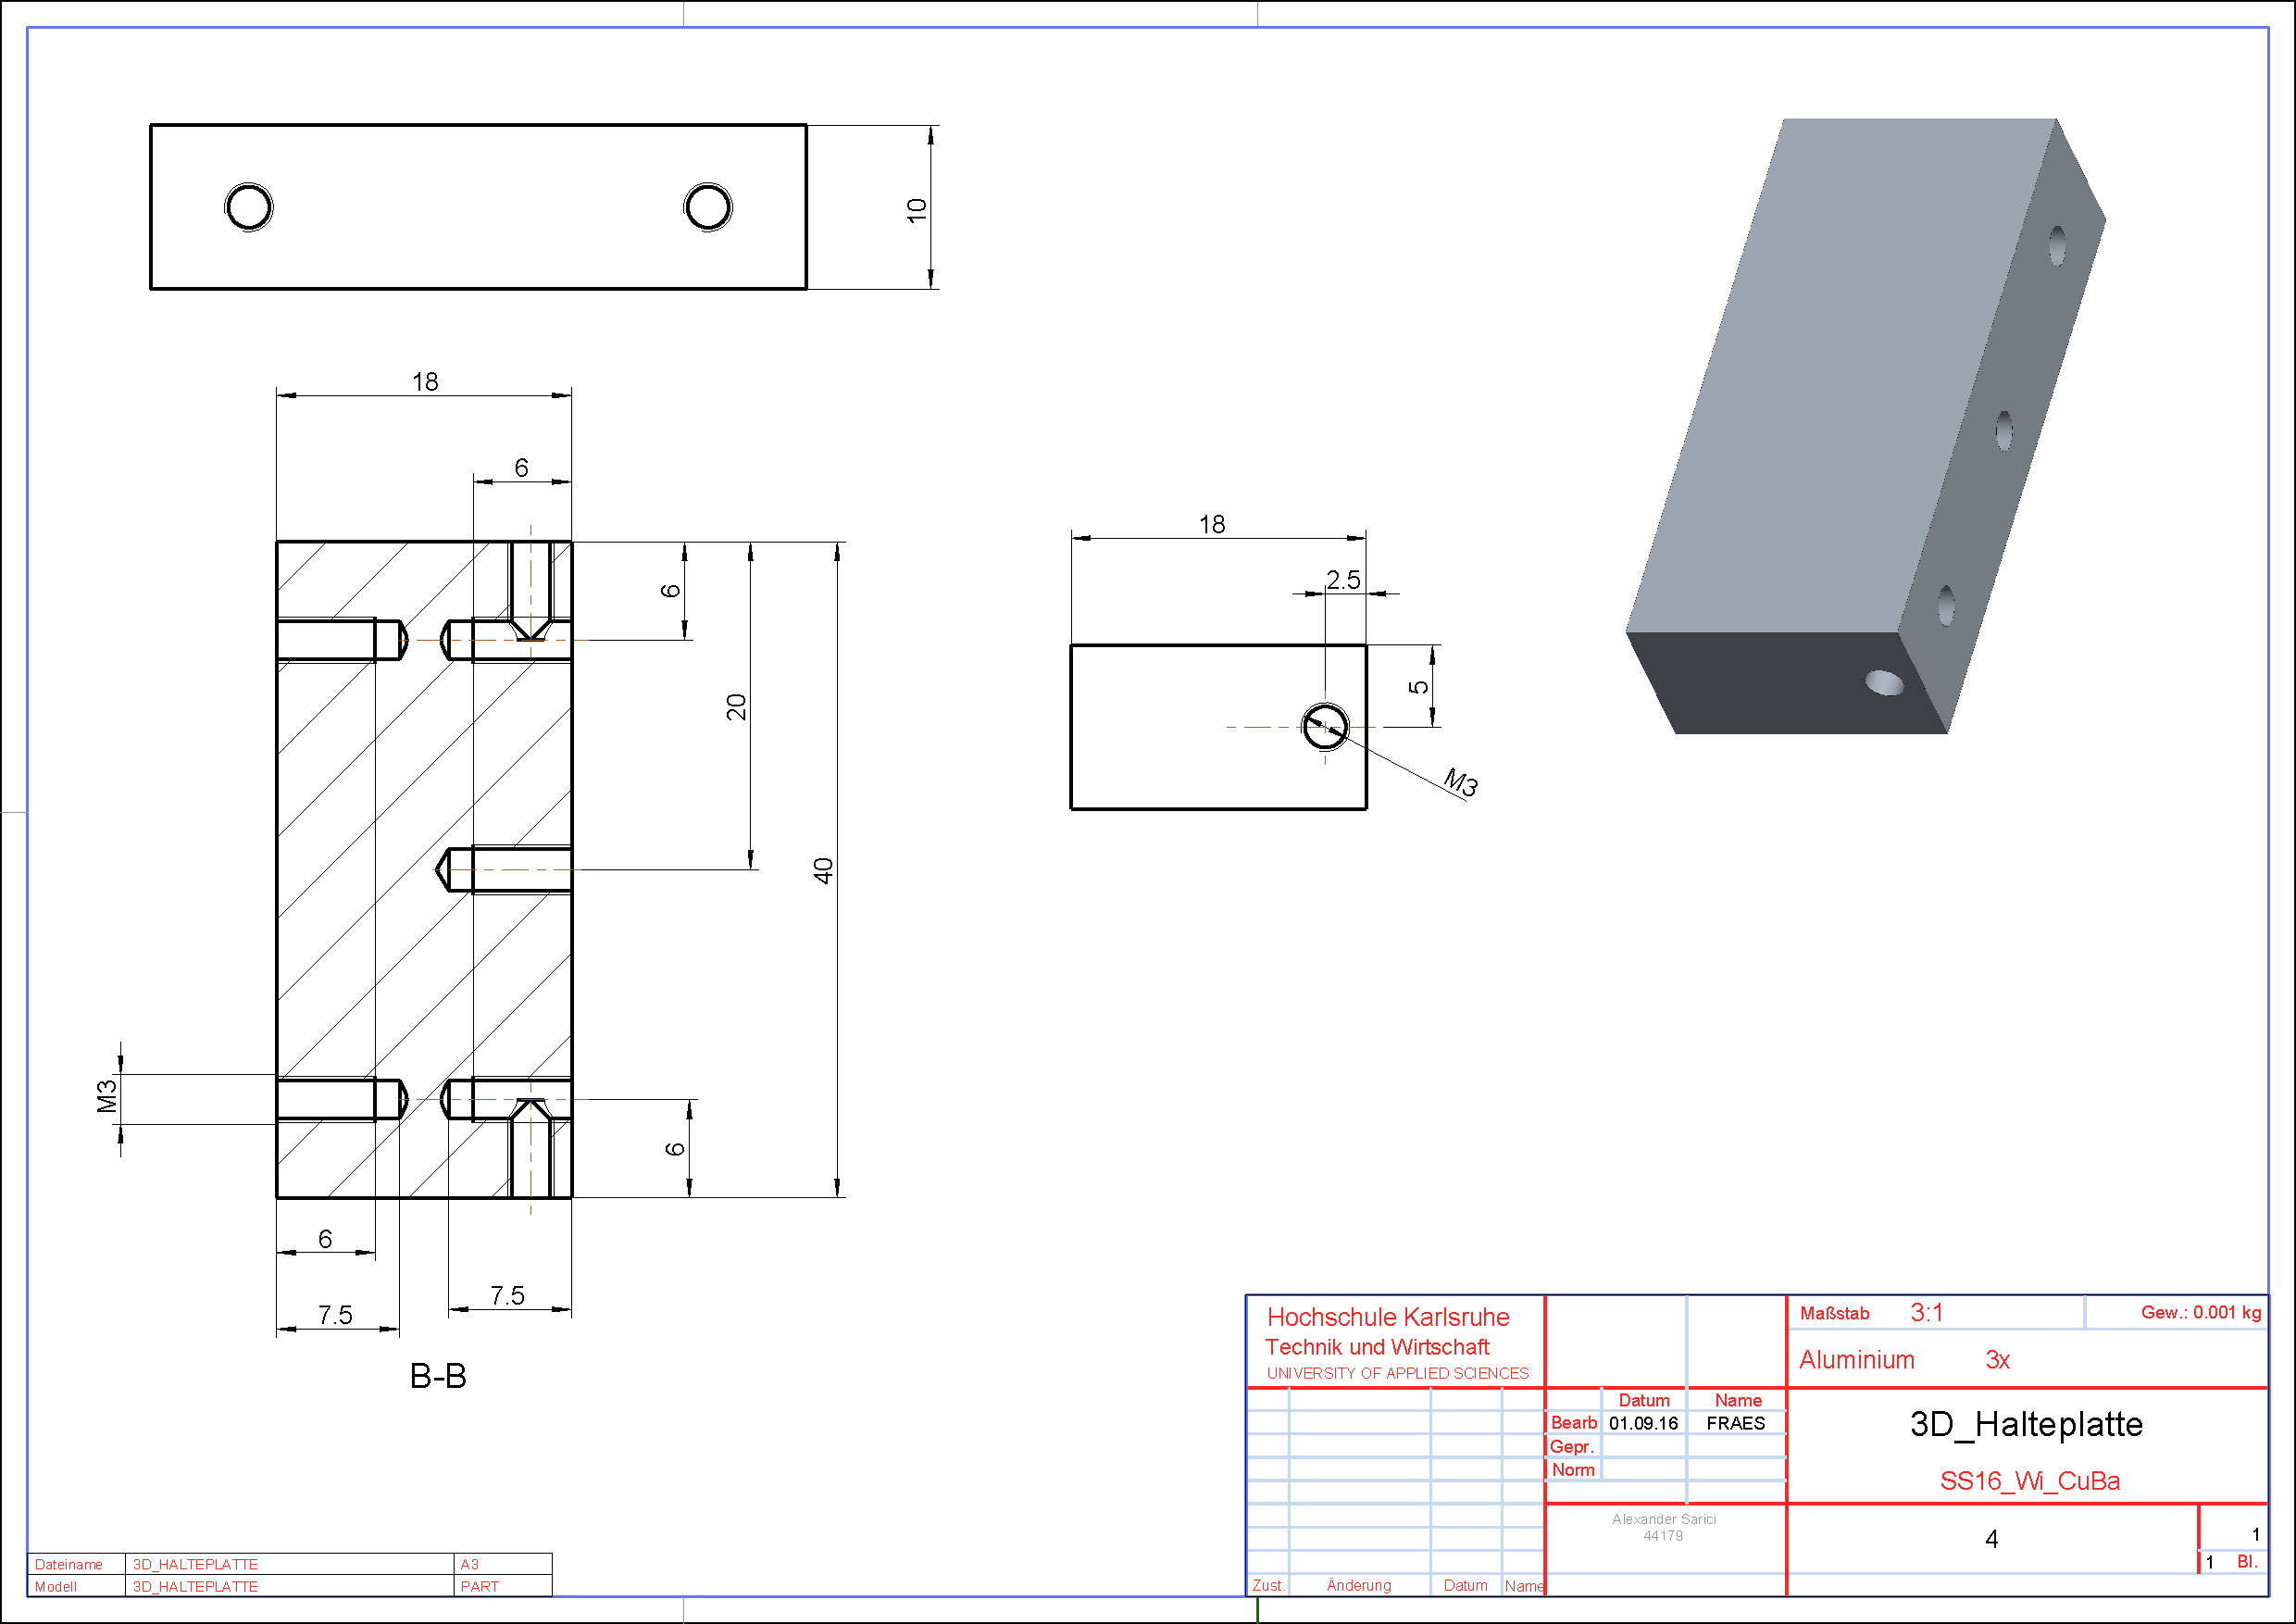
\includegraphics[width=1.5\textwidth]{img/3d_halteplatte.pdf}
	\end{center}
	\caption{Technische Zeichnung Halteplatte, Quelle: eigene Darstellung}
	\end{figure} 
	
	\begin{figure} 
	\begin{center}
	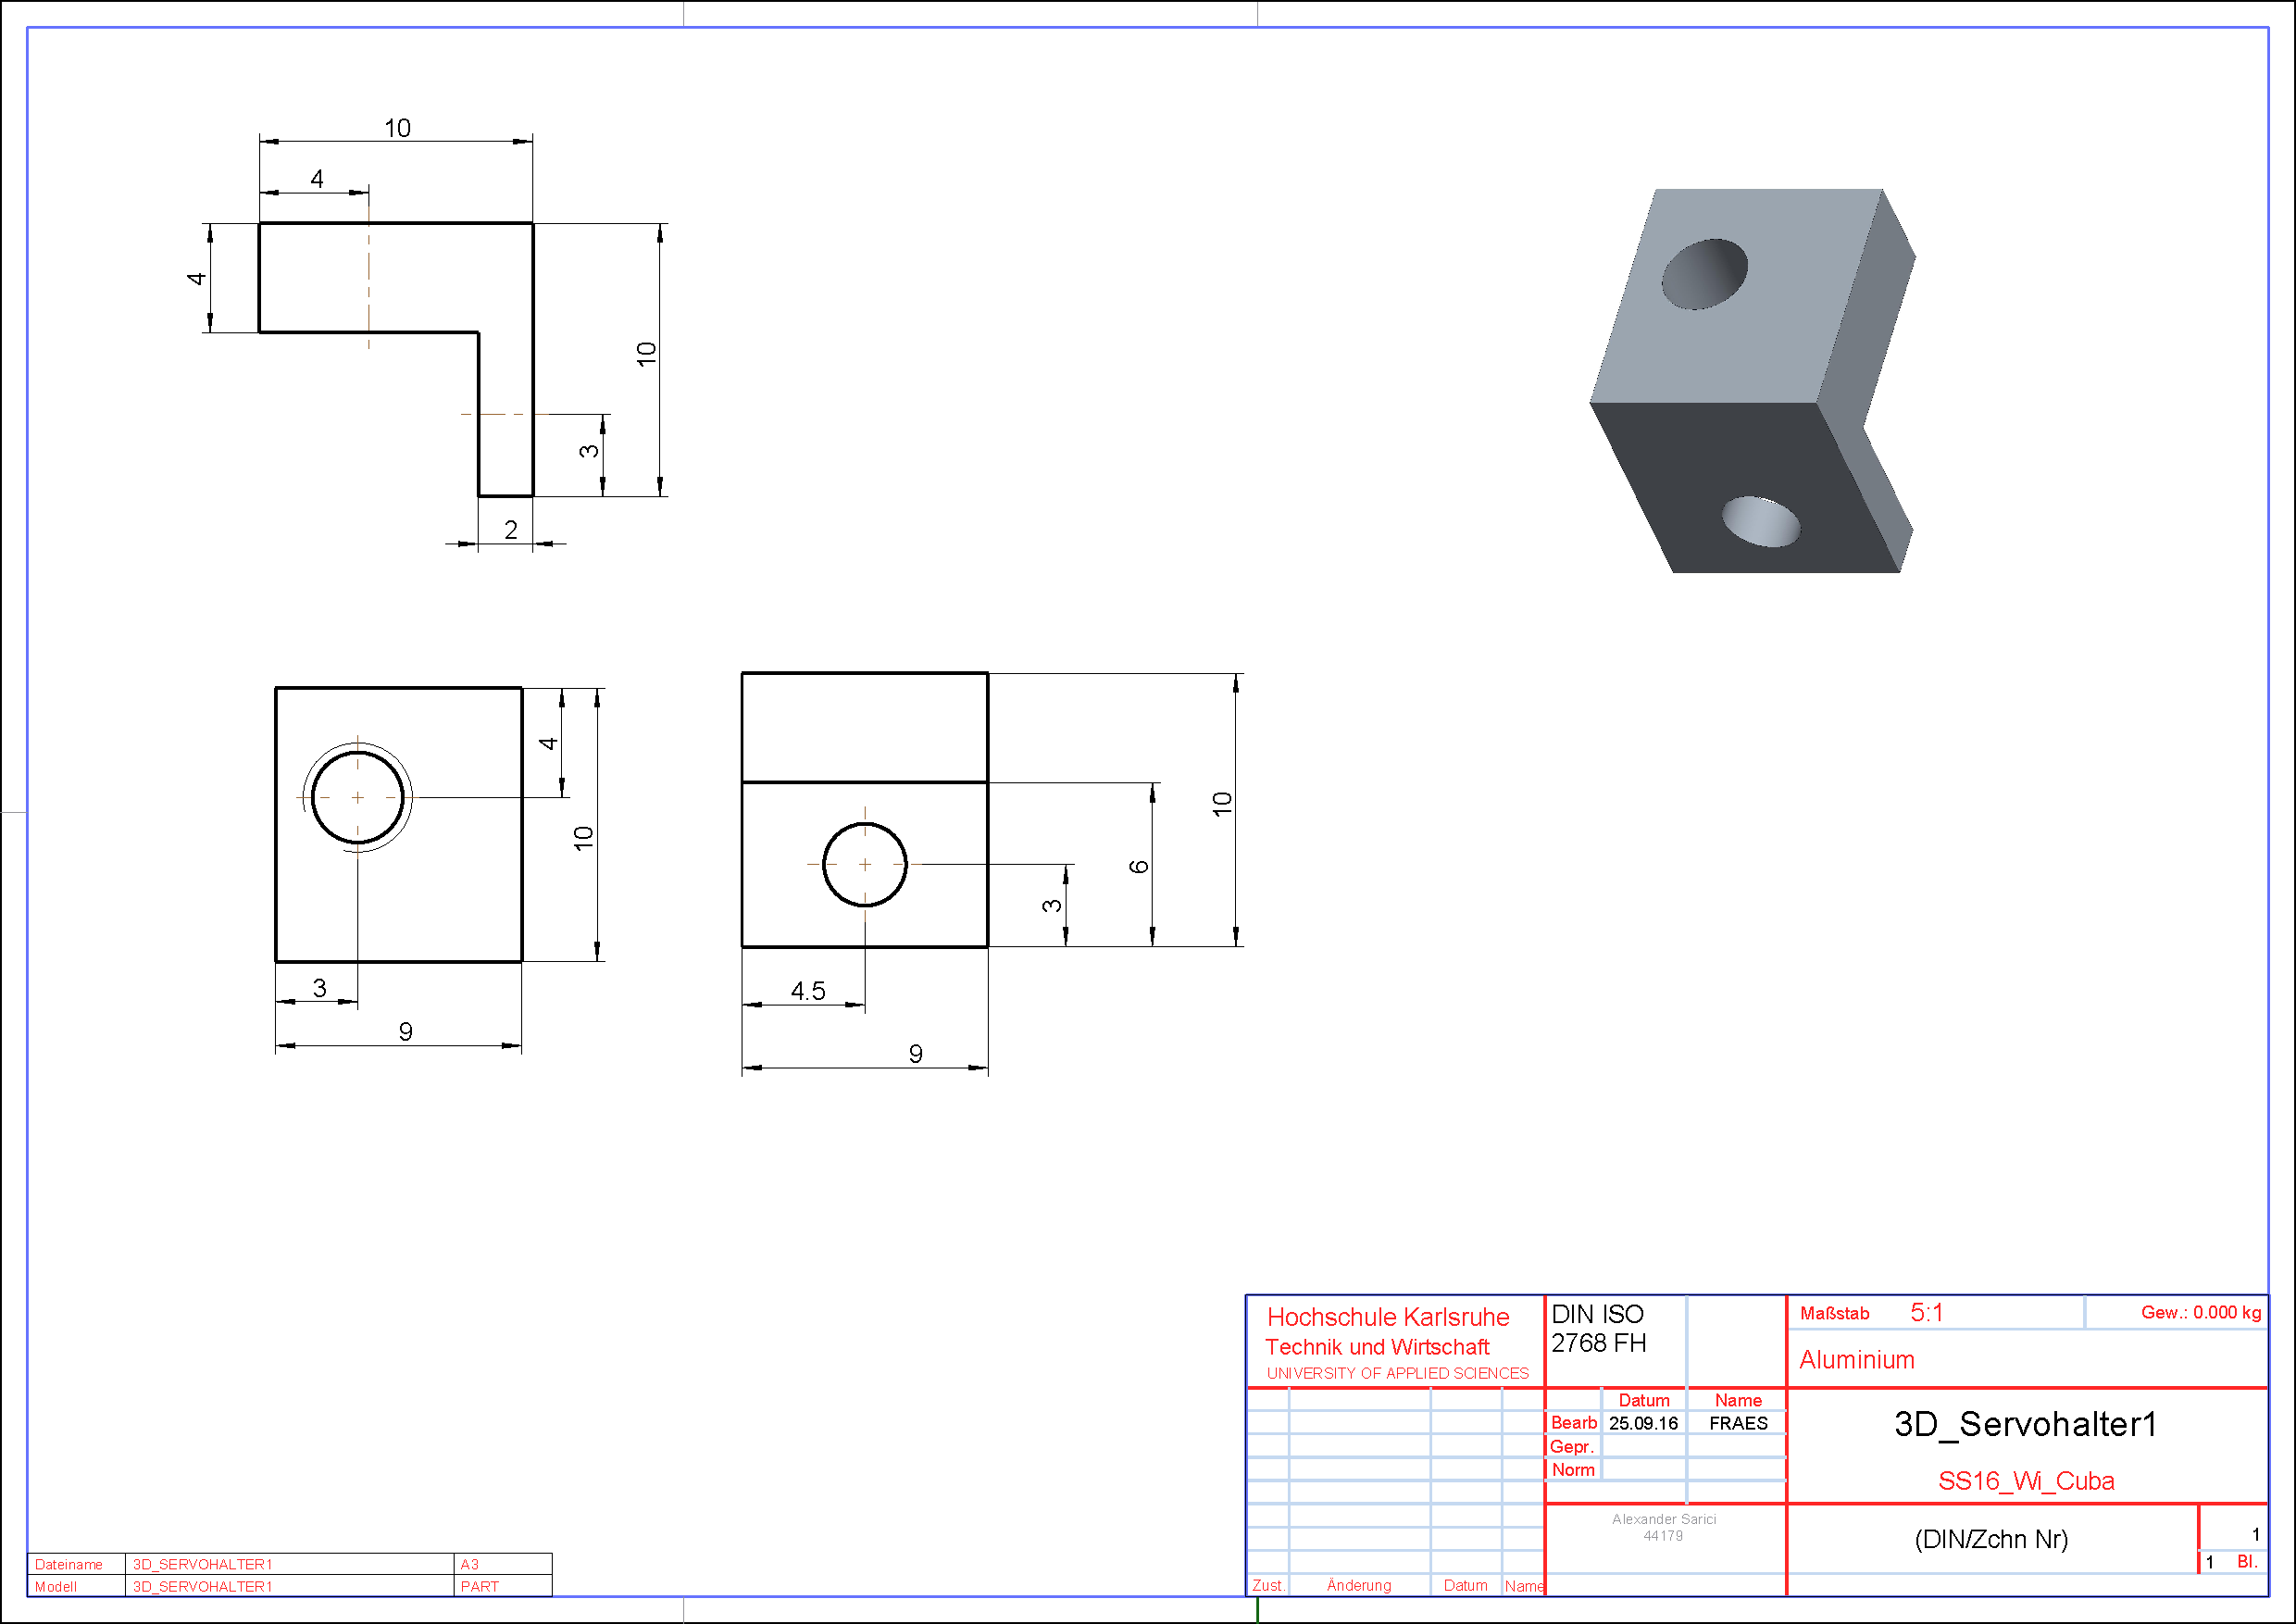
\includegraphics[width=1.5\textwidth]{img/3d_servohalter1.pdf}
	\end{center}
	\caption{Technische Zeichnung Servohalter links, Quelle: eigene Darstellung}
	\end{figure} 
	
	\begin{figure} 
	\begin{center}
	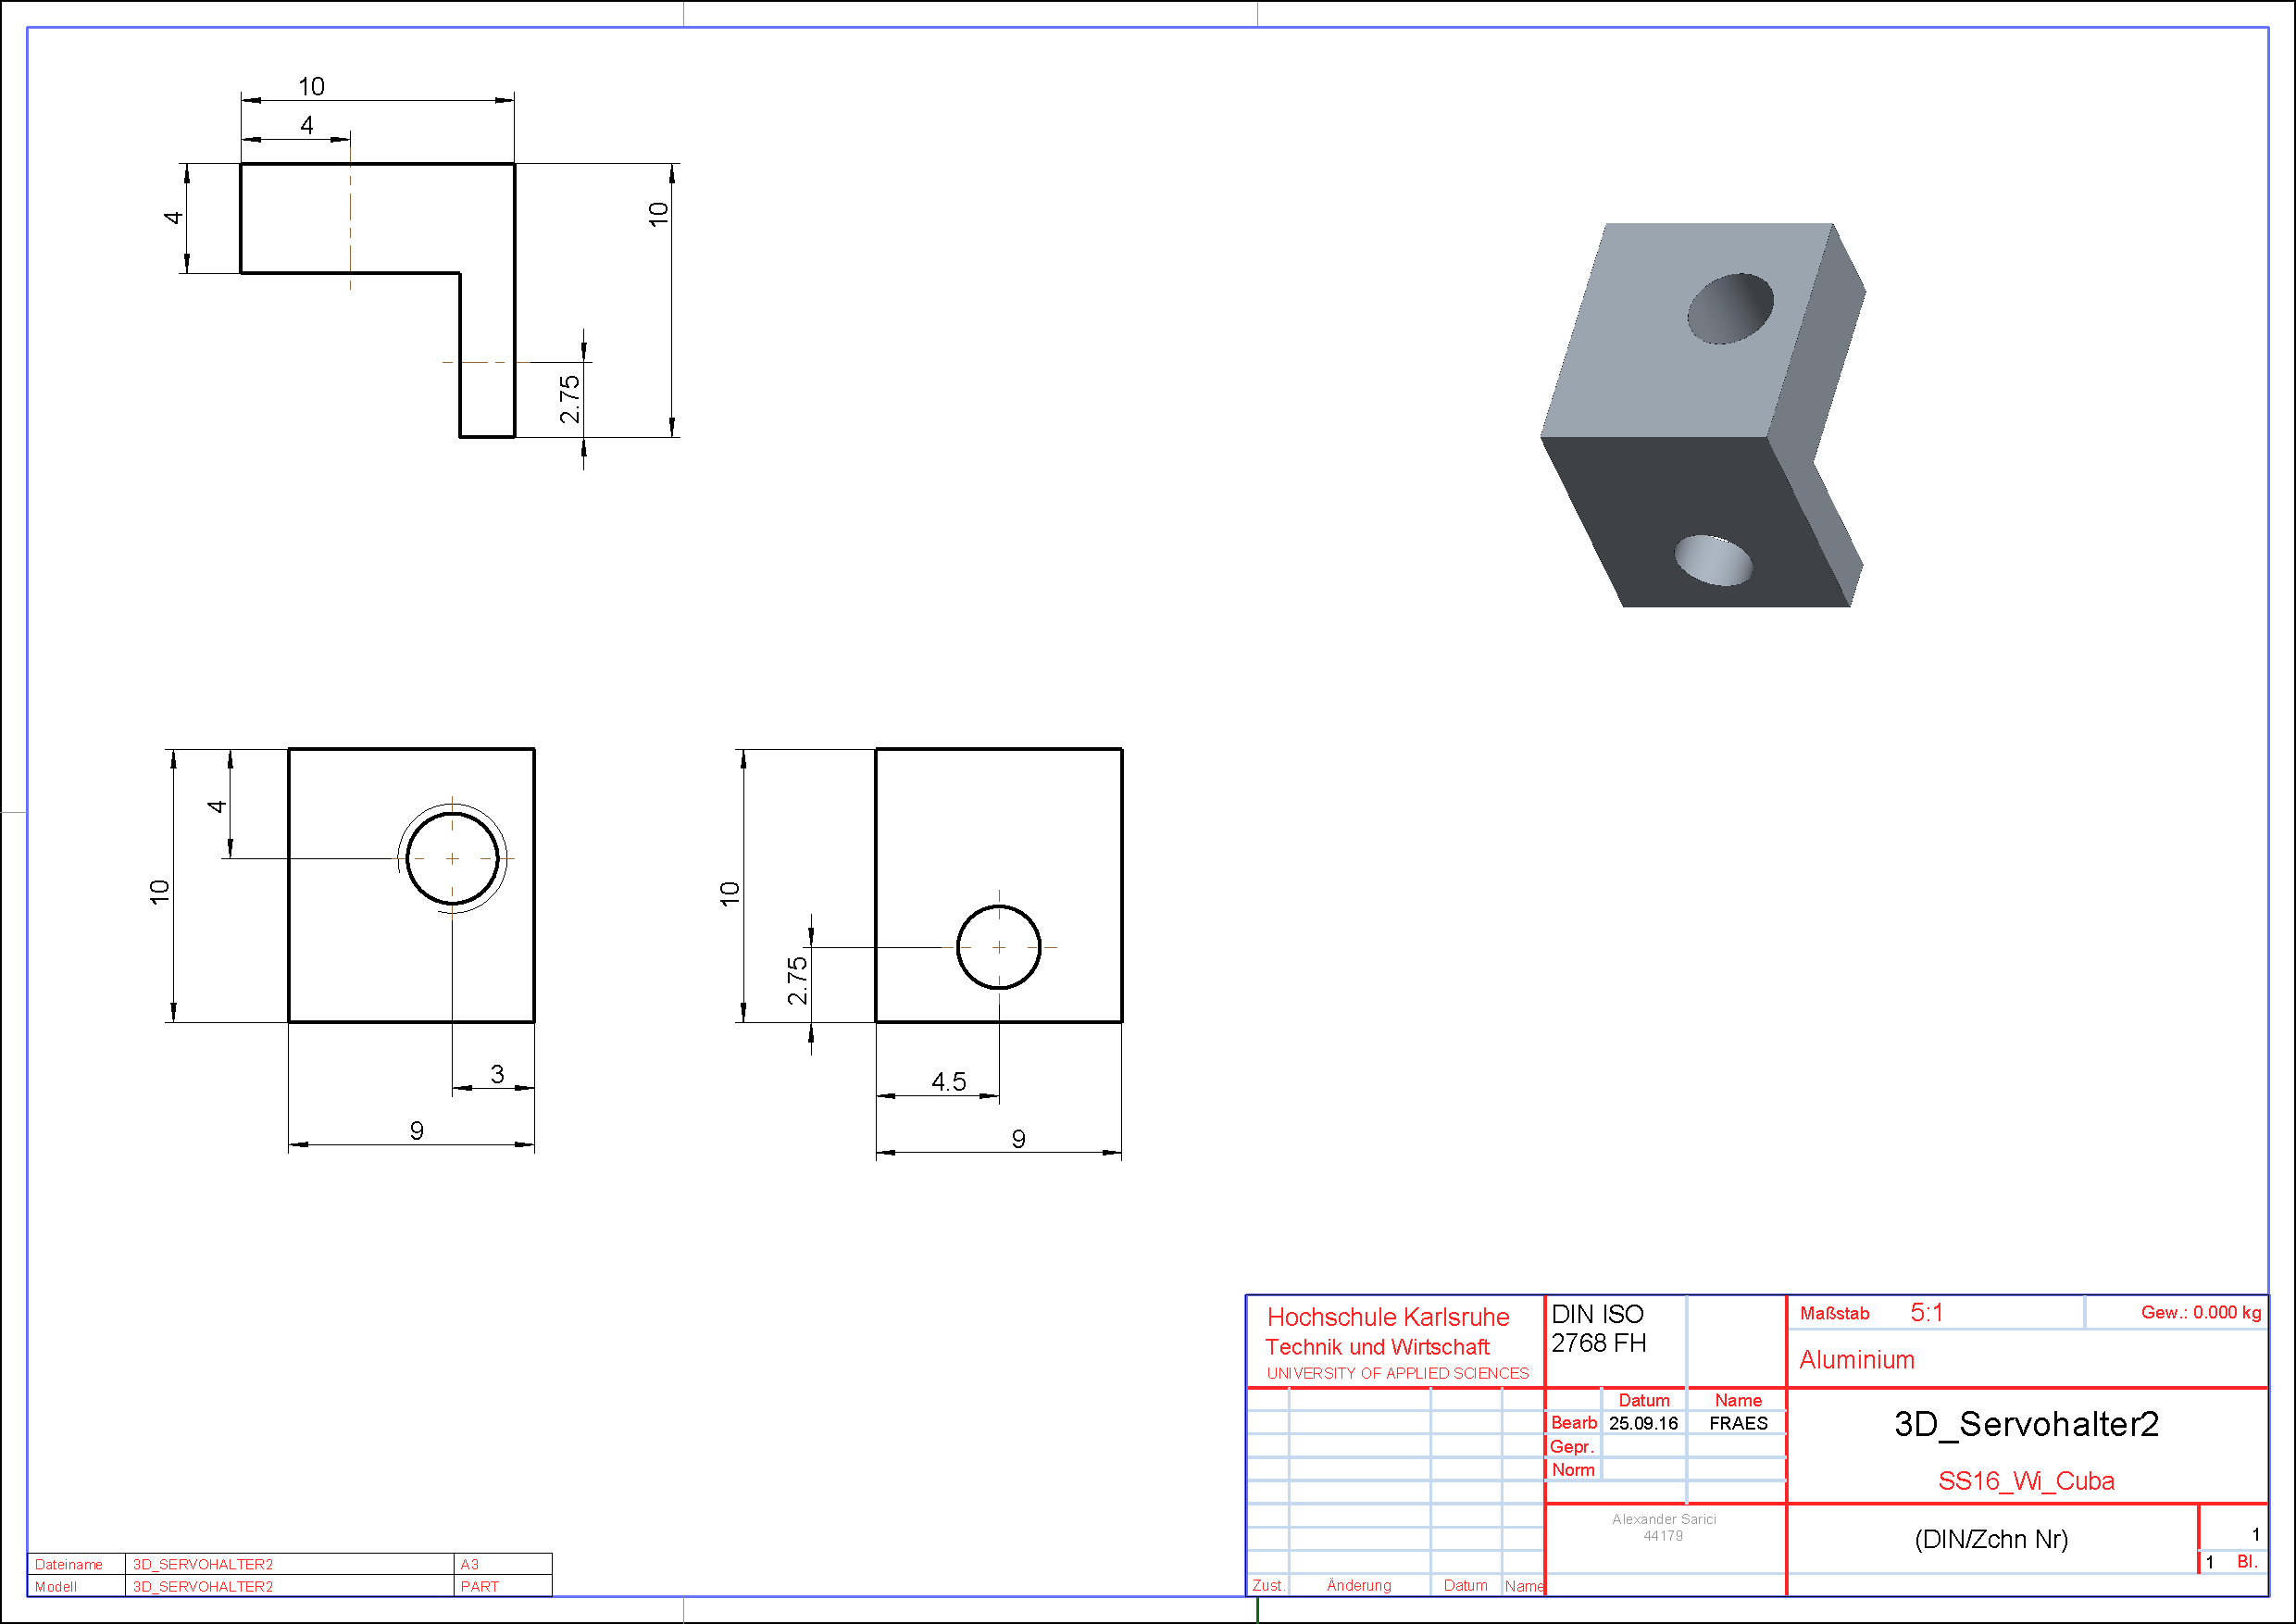
\includegraphics[width=1.5\textwidth]{img/3d_servohalter2.pdf}
	\end{center}
	\caption{Technische Zeichnung Servohalter rechts, Quelle: eigene Darstellung}
	\end{figure} 
		
	\begin{figure} 
	\begin{center}
	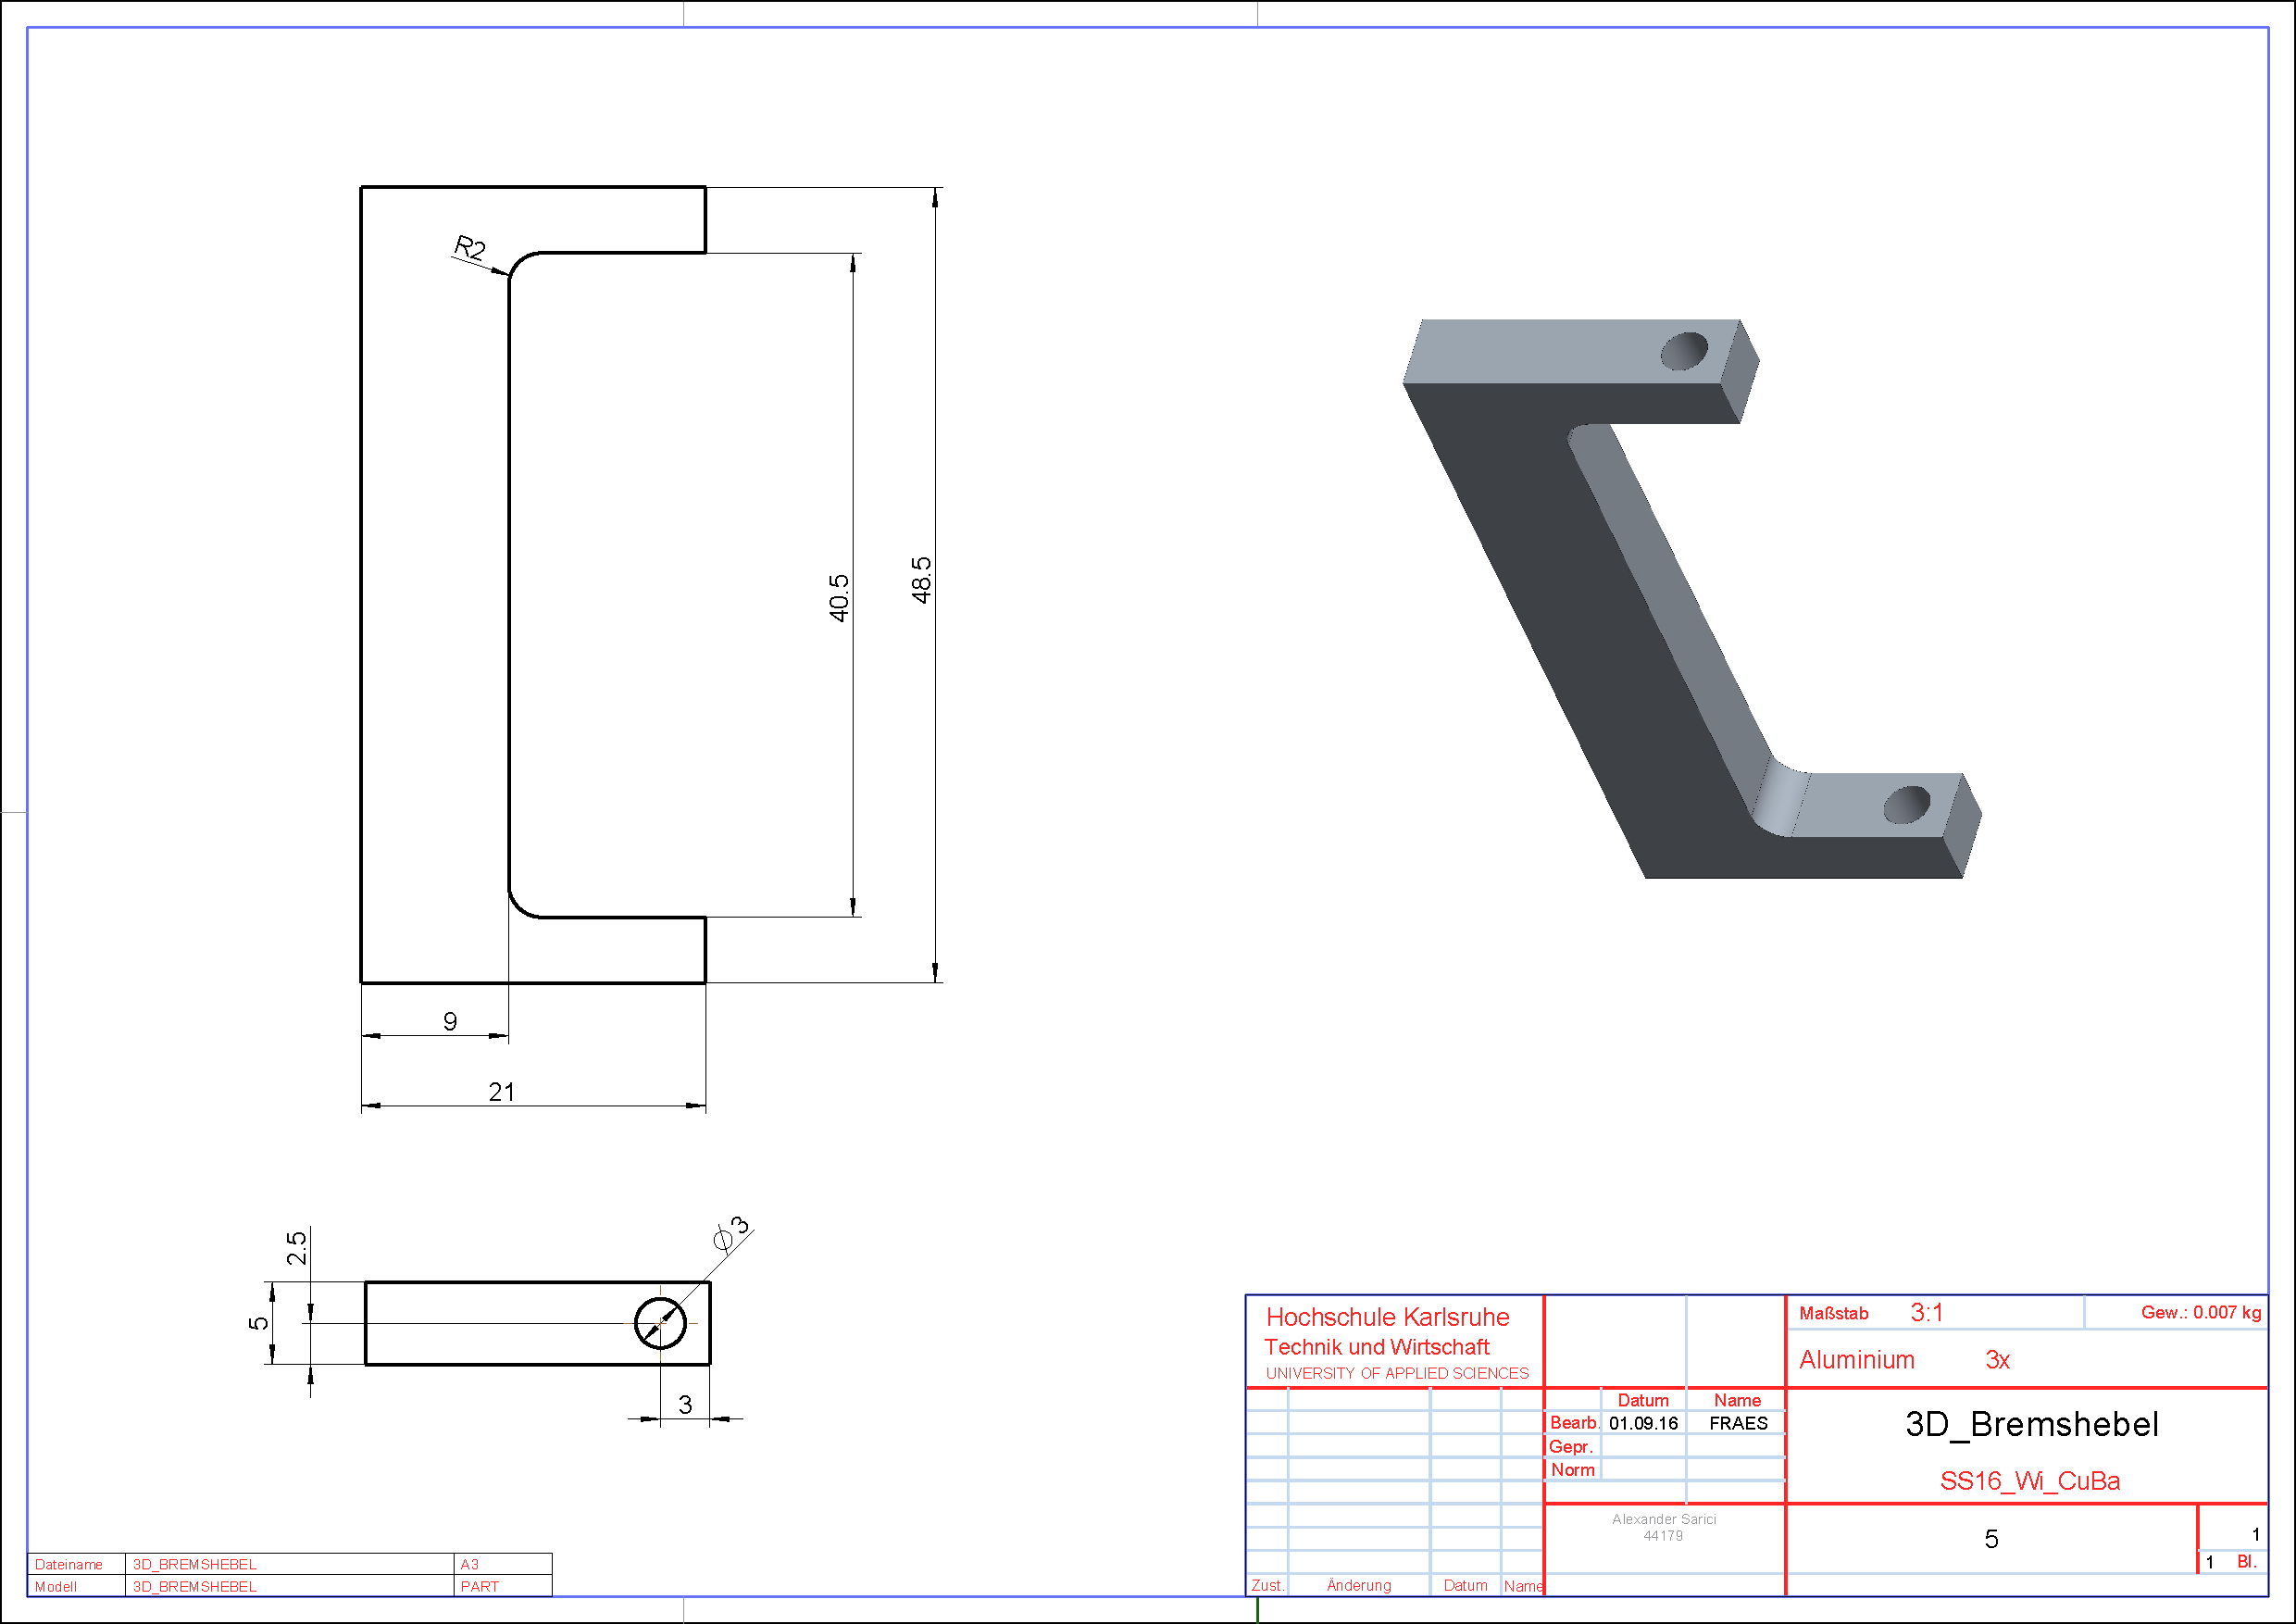
\includegraphics[width=1.5\textwidth]{img/3d_bremshebel.pdf}
	\end{center}
	\caption{Technische Zeichnung Bremshebel, Quelle: eigene Darstellung}
	\end{figure}  
	
		
	\begin{figure} 
	\begin{center}
	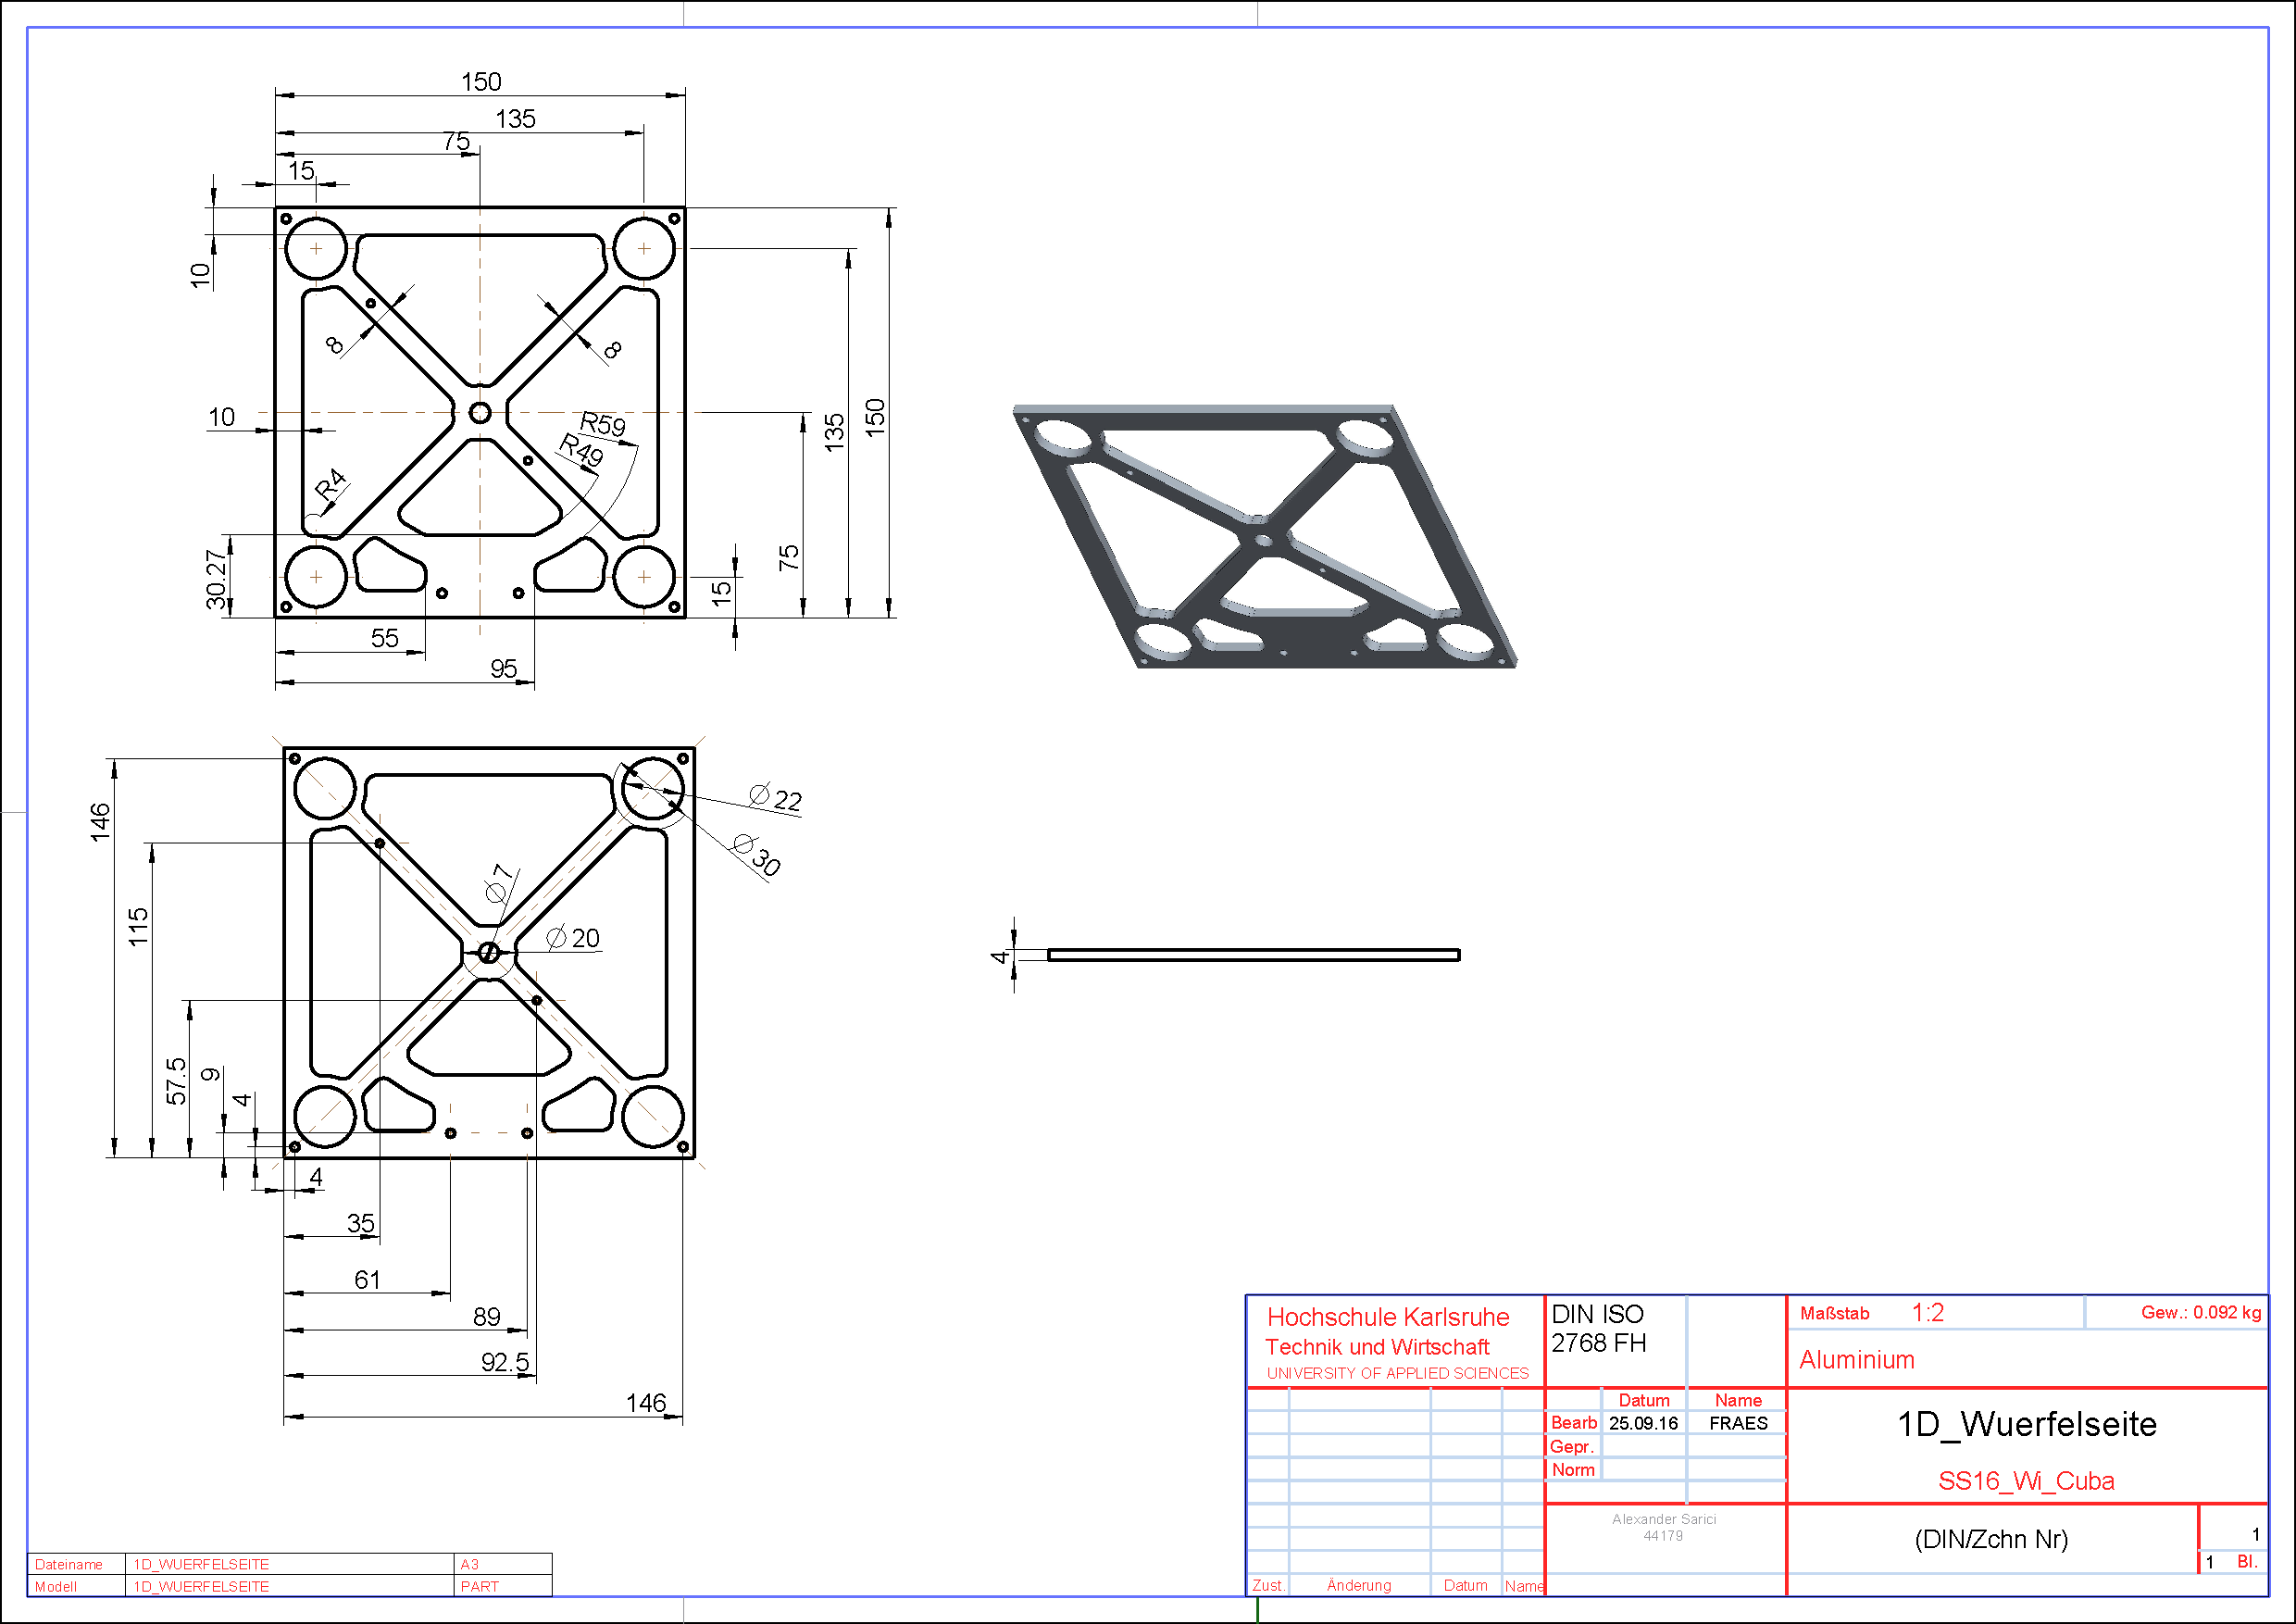
\includegraphics[width=1.5\textwidth]{img/1d_wuerfelseite.pdf}
	\end{center}
	\caption{Technische Zeichnung Würfelseite, Quelle: eigene Darstellung}
	\end{figure}  
	
\end{landscape}

\end{document}